\documentclass{openjournal}

\usepackage[T1]{fontenc}
\usepackage{graphicx}
\usepackage{amsmath,amssymb}
\usepackage{hyperref}
\usepackage{tabularx}
\usepackage{booktabs}
% suppress the class's end-of-document template advertisement;
% delete this block to restore it
\makeatletter
\renewenvironment{bottompar}{\setbox\z@\vbox\bgroup}{\egroup}
\makeatother

\shorttitle{An ALMA Archival Technosignature Search within 40\,pc}
\shortauthors{White \& Dey}

\begin{document}

\title{A Search for Time-Variable and Frequency-Drifting Narrowband
Technosignatures toward ALMA-Observed Stars within 40\,pc of the Sun:
Survey Design and First Results}

\author{Glenn J. White\altaffilmark{1,2} and Robin Dey\altaffilmark{3}}
\altaffiltext{1}{School of Physical Sciences, The Open University, Walton Hall, Milton Keynes, MK7 6AA, UK; glenn.white@open.ac.uk}
\altaffiltext{2}{RAL Space, STFC Rutherford Appleton Laboratory, Harwell Campus, Didcot, OX11 0QX, UK}
% TODO (AUTHOR INPUT, referee R2-m1): complete the VBRL Holdings Inc.
% affiliation (city, country) and add an Acknowledgements/competing-interest
% statement disclosing Robin Dey's employment relationship to VBRL and whether
% VBRL funded or otherwise supported this work. Cannot be authored by the
% assistant -- awaiting the authors' wording.
\altaffiltext{3}{VBRL Holdings Inc.}

\begin{abstract}
We have searched public archival ALMA observations of a volume-limited
census of 168 stars within 40\,pc of the Sun for narrowband
technosignatures. We find no evidence for a technosignature in any of
the data searched. The experiment constrains carriers that are
time-variable on the timescale of an observing track and/or drift in
frequency: the per-channel temporal-median subtraction that rejects
stationary ground-based interference also suppresses phase-steady
carriers, so a stable beacon lies outside the class this pipeline can
constrain, and we make no statement about it. At the epoch of this
release, 104 of 208 planned star/band datasets across 85 census stars
(79 independent systems) have been searched to completion: 417
spectral windows spanning 1.3--38.8\,pc and 92.4\,GHz of unique sky
frequency between 89.6 and 495.1\,GHz. Every window's stellar position
is compared with 512 control positions carried through an identical
search, which calibrates the false-alarm rate empirically rather than
assuming Gaussian statistics. Four windows pass the joint criterion:
three are circumstellar CO (two toward $\beta$~Pictoris, one toward
HD~48370) and one, toward CP$-$72~2713, is a marginal crossing
consistent with the 0.8 flags expected by chance across 417 windows.

Nominal $5\sigma$ detection thresholds span
$1.6\times10^{13}$--$2.8\times10^{17}$\,W in EIRP (median
$1.3\times10^{15}$\,W). Because most windows are channelised at
15.625\,MHz these are native-channel power thresholds, not
Hz-resolution narrowband sensitivities. A 1200-trial injection
campaign into real calibrated visibility data recovers the searched
class at $42^{+16}_{-14}$ per cent at the nominal threshold, so these
thresholds must not be read as 95-per-cent completeness limits.
Folding the measured completeness in, and conditioning explicitly on
emission lying inside the searched spectral windows and persisting
through the observed epochs, the zero-detection result bounds the
fraction of systems hosting a transmitter of EIRP $\geq10^{16}$\,W at
$<6.5$ per cent (95 per cent confidence; the 56 systems with
injection-calibrated coverage). Idealised calculations assuming unit
recovery, or a uniform 42-per-cent recovery, would instead give 3.8
and 9.0 per cent; we quote them only as bracketing values. All limits
assume continuous emission: at duty cycle 0.5 the primary bound
weakens to 13 per cent, and by 0.1 it is 65 per cent and effectively
vacuous.
\end{abstract}

\keywords{extraterrestrial intelligence, radio lines: stars, submillimetre: stars, surveys, astrobiology}

\section{Introduction}
\label{sec:intro}

A technological civilisation, whether deliberately signalling or
simply going about its own affairs, may leave a detectable imprint on
the electromagnetic spectrum: a \emph{technosignature}
\citep{Sheikh2020,SETIreview2025}. Six decades of radio searches have
grown into surveys of many thousands of stars, yet, as
\citet{Wright2018} quantified, they have sampled only an infinitesimal
fraction of the multi-dimensional space of transmitter frequency,
bandwidth, power, and duty cycle. Three gaps persist: the
millimetre and submillimetre regime above ${\sim}50$\,GHz is
essentially unsearched; most surveys target interest-selected classes
of star rather than the local stellar population; and few studies have
systematically reprocessed \emph{existing} interferometric archives.

This paper addresses all three. We construct a census of every star within 40\,pc of the Sun with
public ALMA archival coverage,
irrespective of spectral type, disc-hosting status, or known planets,
and mine that archive for narrowband technosignature candidates and
anomalous millimetre continuum, correcting for stellar proper motion
and for the Doppler drift rates plausible for a transmitter on an
orbiting platform. The search class is set by the processing itself, which suppresses
phase-steady carriers, so this paper constrains \emph{time-variable
and/or sufficiently frequency-drifting narrowband emission} only
(Appendix~\ref{app:inject} measures both sides of that definition).
Four archival-specific analyses supplement the classical search:
closure-phase vetting, a continuum anomaly screen, a chirp and
periodicity re-analysis, and a cross-target frequency-occupancy check.

Per-target tables are deferred to online-only
Appendix~\ref{app:table}. We publish at 41 per
cent completion because the citable content is methodological -- the
census definition, the empirically calibrated false-alarm machinery,
and the measured completeness -- together with a first set of
per-target limits, every number tied to a frozen pipeline and a named
data snapshot that later work will supersede row by row without
invalidating this one.

\section{Background}
\label{sec:background}

Six decades of searches divide into wide-field commensal surveys and
targeted programmes on preselected stars, the modern generation
dominated by Breakthrough Listen, whose GBT, Parkes, and MeerKAT
programmes have published multi-thousand-star limits from 1.1 to
8\,GHz \citep{BLoverview,Enriquez2017,Price2020,BLMeerKAT2026}, with
parallel efforts on FAST, LOFAR, NenuFAR, the Sardinia Radio
Telescope, and commensal VLA, MeerKAT, and MWA back-ends
\citep{Zhang2020,LOFARdualsite2023,SRT2025,Tremblay2024};
machine-learning rejection of RFI-dominated hit lists has become
central \citep{Ma2023,Choza2024,GLOBULAR2025,AnomalyParkesGBT2025,
BRaTs2026} -- a capability the classical threshold search we adopt
lacks (\S\ref{sec:discussion}). Two structural points shape the
present survey. First, \citet{Margot2023} showed that a non-detection
bounds the transmitter fraction only if the sample is representative
of the underlying population -- a condition interest-selected samples
violate. Second, essentially all of this activity lies below
${\sim}10$\,GHz: above it, the millimetre and submillimetre regime has
been searched only once before, also with ALMA \citep{Mason2024};
sixteen programmes are tabulated in Appendix~\ref{app:priorsurveys}.

\citet{Mason2024} searched archival Band~3 windows toward 28
``stellar bycatch'' stars and placed EIRP$_{\rm min} >
7\times10^{17}$\,W for the nearest, identifying the challenges of
high-frequency work: drift rates scale with observing frequency,
smearing erodes sensitivity unless a drift search is run, and the
molecular line forest confuses. Our earlier pilot
(\citealp{White2026}; under review at the time of submission -- the
citation is provisional and will be updated on acceptance) extended
that methodology to TRAPPIST-1 across Bands 3, 6, and 7
(EIRP$_{\rm min}\sim5$--$10\times10^{13}$\,W, no detection) and built
the ranked 100-star list from which this survey grew. The incremental
content of this submission is the census selection
(\S\ref{sec:sample}), the 512-position control-ring
false-alarm calibration, closure-phase vetting, the
spectral-type-normalised continuum screen, the chirp and periodicity
extension, and the cross-target frequency-occupancy check.
% TODO (AUTHOR INPUT, for the editor's cross-check request): confirm the
% EB-by-EB overlap between this paper and White (2026) -- which execution
% blocks appear in both, and whether any number printed here is also
% printed there. Draft statement below; verify against the White (2026)
% manuscript before submission and complete the bracketed clause.
No execution block is analysed in both papers: the pilot's 100-star
search products are superseded, not re-used, here, and every window
analysed in this paper was re-reduced and re-searched from the raw
archive data with the pipeline of \S\ref{sec:method}.
% AUTHOR: confirm the single deliberate exception, if any -- e.g.\ shared
% calibrator-only usage -- and state it here; otherwise delete this
% bracket and the sentence stands as the complete answer.

Figure~\ref{fig:context} places this release's nominal EIRP thresholds
among the published searches under two conventions. A quoted EIRP
threshold is defined at the producing survey's channel width, and
those widths span nearly six orders of magnitude between Hz-scale
backends and ALMA's native correlator channels: panel~(a) divides each
limit by its native channel width to give W\,Hz$^{-1}$, the
like-for-like spectral comparison (the primary panel), and panel~(b)
is the total-power comparison -- our limits are numerically comparable
to the deepest L-band limits in panel~(b) only because the nearest
targets lie an order of magnitude closer, despite channels some
$10^{6}$ times coarser. Our linewidth convention is set out in \S\ref{sec:method}.

\begin{figure*}
\centering

\includegraphics[width=\textwidth]{figures/eirp_context.pdf}
\caption{Literature context of this release's nominal thresholds.
(a) Spectral power threshold (W\,Hz$^{-1}$), the primary and
like-for-like comparison: the same literature points carry over
unchanged (one-Hz channels make their quoted EIRP and spectral power
identical), while our kHz--MHz channels separate the two by up to six
orders of magnitude -- this survey (blue; nominal 5$\sigma$
thresholds under the boxed reading rule of \S\ref{sec:method})
against \citet{Enriquez2017} (orange diamonds), \citet{Margot2023}
(aqua squares), \citet{Mason2024} (violet triangles).
(b) Total transmitter power required for detection at each survey's
native spectral resolution -- not narrowband spectral sensitivity --
with the deepest per-target limits of \citet{Price2020} as left-edge
ticks; the grey dotted line marks EIRP $\propto d^{2}$, the green
dashed line an Arecibo-like planetary radar ($2\times10^{13}$\,W).
Conventions differ among surveys (thresholds, drift coverage,
confidence); context, not a ranking.}
\label{fig:context}
\end{figure*}

A non-detection must be translated into a quantitative exclusion
statement. \citet{Wright2018} formalised the ``Cosmic Haystack''
search volume; \citet{Margot2023} its conversion into an upper bound on the
transmitter-hosting fraction; and
\citet{EarthDetectingEarth2025} asked instead where Earth's own
technosignatures would be detectable -- a calibration point any
survey's sensitivity can be read against.

The case for a census over interest-selected lists follows directly:
most surveys select by proximity, spectral type, planets, or Earth
Transit Zone membership, which is reasonable per unit time. The
ALMA-specific form is
disc selection: ALMA-detected discs are orders of magnitude brighter
than the Solar System's zodiacal cloud would appear at interstellar
distances, so disc-selected samples skew young and dynamically
active. This survey therefore identifies every star within 40\,pc in the
usable field of at least one public ALMA observation
(\S\ref{sec:sample}) -- a bycatch census of the ALMA-observed subset of the local stellar
population within a fixed volume, which is not the same thing as a
census of that population. It removes technosignature-specific selection, not the
astrophysical selection embodied in the archive itself; our 168 stars are ${\sim}7$ per cent of the known stellar population
within 40\,pc,
and that residual coverage selection is characterised as a
completeness function (\S\ref{sec:sample},
Table~\ref{tab:searchspace}) rather than left implicit.

The coming decade will widen the search: the SKA
\citep{SKA2015,SKA2026review} and ngVLA \citep{ngVLASETI2022} bring
wide bandwidth and commensal architectures below ${\sim}50$\,GHz, but
neither offers ALMA's combination of resolution and collecting area
above it in the near term, so a systematic mm/submm census remains an
ALMA-specific measurement for some years.

\section{Sample selection}
\label{sec:sample}

Our sample comprises every star within 40\,pc of the Sun (Gaia~DR3
parallaxes, all distances direct inversions $d = 1/\pi$; every entry
has $\pi \ge 25$\,mas with $\sigma_\pi/\pi \le 0.8$ per cent) with
at least one public ALMA observation whose proper-motion-corrected
position at the epoch of observation falls within the field of view of
at least one execution block -- not necessarily at the pointing centre, since mosaics and
wide pointings serendipitously cover more than one catalogued star.
No disc, planet, or spectral-type weighting is applied; those
properties are descriptive metadata, not selection criteria. This identifies 168 unique target stars, processed
nearest-first -- a sensitivity-ranked order, not an unbiased draw, on
which the prevalence statements of \S\ref{sec:discussion} are
conditional.

The composition follows from this archival selection: just under two
thirds of the 168 stars are M~dwarfs (76 stars, 63 per cent),
followed by 12~K, 11~G, and 8~F~dwarfs, a single A-type star
($\beta$~Pic), and six white dwarfs; six faint companions lack
tabulated types. Fifteen of the 46 processed stars are confirmed exoplanet hosts
(\S\ref{sec:discussion}), and debris-disc hosts ($\beta$~Pic, AU~Mic, $\epsilon$~Eri, $\tau$~Cet)
contribute continua that include circumstellar dust, which the
continuum lane's spectral-type-normalised screen (\S\ref{sec:method})
keeps from masquerading as an anomaly.

What the sample covers should be explicit: the 168 stars are every star within 40\,pc with public ALMA coverage,
so the census is complete with respect to the intersection of the
40-parsec reference catalogue with the public-archive snapshot (2026 September~8) that
defines this release, and conditional on that intersection only.
Against the
reference Gaia~DR3 catalogue of the solar neighbourhood
(Figure~\ref{fig:sample}, online-only appendix; 17\,566 stars within
40\,pc passing the parallax-quality cut of
Table~\ref{tab:selfunc}), the 168 stars are ${\sim}1$\%. That reference list is itself incomplete at
both ends, so the denominator is a convention, and we use the fraction
only to say it is small. How the covered stars differ from the census is quantified
in
Table~\ref{tab:selfunc} (online-only appendix), so the selection function is inspectable rather than asserted: a strong enrichment of the nearest systems falling towards parity with
distance, mild M-dwarf depletion with F/G enrichment, and
planet-hosting in 20 of the 168 census entries. Age and
disc-hosting flags are not uniformly available for the census and are
documented qualitatively, with a machine-readable selection-function
table part of the release.

ALMA coverage is itself strongly astrophysically selected -- it
inherits the proposers' interests -- so any prevalence statement this
survey makes concerns the ALMA-observed subset of the solar
neighbourhood, not the neighbourhood as a whole. The stellar counts quoted throughout are
catalogue-entry counts: the 120 entries comprise 113 distinct physical
systems (seven designation-linked component
pairs),\footnote{Component designations follow SIMBAD; in
the per-target file (Appendix~\ref{app:table}) each entry carries its own row and distance, and
spatially unresolved pairs (e.g.\ the UV~Ceti entries at 2.7\,pc,
whose fluxes are blended) are marked in the notes column.} and because
the 44 narrowband-covered entries include the spatially unresolved
UV~Ceti and AT~Mic pairs, the 104 star/band datasets, 417 windows, and 57
execution blocks derive from 42 independent systems -- the paired rows
are bookkeeping, not independent trials.

``Usable public ALMA coverage'' is frozen as a five-criterion
decision tree, enforced for this release and not changed subsequently
without an erratum: (i) at least one public execution block (EB) with
QA2-calibrated visibilities covering the star's epoch-propagated
position in the primary beam, with no minimum integration,
sensitivity, antenna count, mosaic-tile count, or array configuration
imposed beyond QA2 state itself; (ii) propagated position within one
primary-beam FWHM of the field centre (largest accepted offset
${\sim}0.7$ FWHMs, Sirius~B); (iii) each spectral window admitted
individually, on the pipeline's quality vetting alone; (iv) no
programme-category restriction -- science, calibration, and
observatory projects enter on identical terms; and (v) a fixed
archive snapshot date (2026 September~8), re-evaluated only at
release boundaries. No star or window was excluded by any criterion
not listed here, and none for short integration (the shortest
retained are 1.0 and 1.5\,min).

Pointed versus serendipitous coverage is quantified from ALMA project
metadata: almost every narrowband-covered star is the pointed science
target in at least one of its execution blocks, the exceptions being a
small number of blocks that point at another programme's science field
or are calibrator-only executions -- leaving Wolf~219 the sole
genuinely serendipitous star. The residual selection function of an archival census is the union of
individual ALMA target lists -- a contrast with interest-selected
technosignature samples that is one of degree, but of
\emph{quantified} degree: a bycatch fraction of 1 star in 44, 1 EB in
57.



\section{Data and methodology}
\label{sec:method}

Survey-specific vocabulary -- target/band dataset, spectral window,
execution block, control ring, candidate, molecular-line exclusion
mask -- is defined once in Table~\ref{tab:glossary}, Appendix~\ref{app:glossary}.

The design is summarised in Figure~\ref{fig:pipeline}: one shared
archive-ingestion stage feeds two independent search lanes. For each
target we mine the public ALMA science archive for all calibrated (or
locally recalibrated) execution blocks covering the star's
Gaia-propagated position, within a bounded per-target processing
budget, and search the resulting visibilities in (i) the
\emph{primary} lane -- a narrowband, Doppler-drift-corrected search
for technosignature candidates, following \citet{Mason2024} and
\citet{Enriquez2017}, converting each non-detection into an
equivalent isotropic radiated power limit
$\mathrm{EIRP_{5\sigma}} = 4\pi d^{2} S_{\rm min} \Delta\nu$, where
$S_{\rm min}$ is five times the per-channel rms of the searched
window (primary-beam corrected), $\Delta\nu$ its native channel
width, and $d$ the target distance; and (ii) an \emph{ancillary} line-excluded continuum lane
(Appendix~\ref{app:continuum}). Throughout, ``5$\sigma$'' denotes this local instrumental threshold in
the sense of Table~\ref{tab:nomenclature}, calibrated separately and
empirically (\S\ref{sec:technosearch}). The chirp/periodicity extension and the
molecular-line census are defined in Appendices~\ref{app:extended}
and~\ref{app:linecat}; every limit, disposition, false-alarm
calibration and completeness statement derives from the narrowband
lane.

Both lanes exclude catalogued molecular transitions, at tolerances
appropriate to their statistics. The continuum lane masks the eight
common species (CO, $^{13}$CO, C$^{18}$O, HCN, HCO$^{+}$, CS, CN,
SiO) at native resolution before integrating; the narrowband lane
applies a $\pm50$\,km\,s$^{-1}$ stellar-frame velocity exclusion mask
(\S\S\ref{sec:frames},~\ref{sec:technosearch}) to any threshold
crossing, and the same mask defines the effective searched bandwidth
(${\approx}87$ of the 92.4\,GHz unique frequency union). Masked regions reduce
the frequency space a candidate can occupy, not the per-channel noise,
so no threshold in the per-target file is affected by the mask.

All flux densities and EIRP thresholds are Stokes~$I$ quantities, so
the limits apply to total transmitted power independent of
polarisation geometry. What is lost is
diagnostic, not sensitivity -- polarisation is not used as a
discriminator (no Stokes $V$/$Q$/$U$ extraction or circularity test
is performed), and a polarisation-sensitive test is a natural future
addition (\S\ref{sec:futurework}).

\medskip
\noindent\rule{\columnwidth}{0.4pt}
\smallskip
\noindent\textbf{How to read every limit in this paper.}
\emph{Every EIRP$_{5\sigma}$ value here is a nominal, local
instrumental detection threshold: five times the per-channel rms of
the searched window, at that window's native channel width, for a
transmitter at the star's position matching the searched temporal and
spectral morphology -- time-variable on track timescales, since
phase-steady carriers dwelling in one channel for most of the track
are suppressed by the statistic's own continuum subtraction
(Appendix~\ref{app:inject}). It is not a calibrated completeness
limit: the injection campaign measures a recovery of roughly one half
at the threshold itself (EIRP$_{50} = 1.10\,$EIRP$_{5\sigma}$ for the
searched class), rising to 83 per cent at twice the threshold power
(EIRP$_{90} > 2\,$EIRP$_{5\sigma}$; Appendix~\ref{app:inject}). It
is a total-power threshold set by ALMA's coarse native
channelisation, not a Hz-resolution narrowband sensitivity. The same
reading applies to every subsequent ``5$\sigma$'' and to the
per-target file (Appendix~\ref{app:table}); it is stated once here and
not repeated at each occurrence.}
\smallskip
\noindent\rule{\columnwidth}{0.4pt}
\medskip

\begin{figure*}
\centering

\includegraphics[width=\textwidth]{figures/pipeline_schematic.pdf}
\caption{Design of the survey. All public execution blocks on the 168
targets are mined from the ALMA science archive, with positions
propagated to each epoch from Gaia~DR3, and searched along the two
independent lanes described in the text. Solid borders mark validated
components. The validation rail summarises the injection-recovery
(1200 trials, Appendix~\ref{app:inject}), chirp/periodicity, and
frequency-occupancy analyses.}
\label{fig:pipeline}
\end{figure*}

\subsection{The search statistic, and the words used for its output}
\label{sec:statistic}

The primary statistic is formed on extracted spectra, not on images or
on visibilities directly. For a sky position $\mathbf{x}$, the
per-channel time series is median-subtracted along the time axis, the
residual dynamic spectrum is stacked along each trial linear drift
rate $\dot\nu$, and the statistic is the largest resulting
single-channel amplitude in units of that window's noise,
%
\begin{equation}
T(\mathbf{x})=\max_{\dot\nu,\;\nu}\;
\frac{S(\mathbf{x},\nu,\dot\nu)}{\sigma(\mathbf{x})},
\label{eq:tstar}
\end{equation}
%
where $S$ is the drift-stacked flux density in one native channel and
$\sigma(\mathbf{x})$ is a single robust scale per position and window,
estimated as $1.4826\times$ the median absolute deviation of that
position's median-subtracted spectrum over all channels, so it is
local in position and global in frequency.
$T_\star \equiv T(\mathbf{x}_\star)$ at the proper-motion-propagated
stellar position; the identical operation, with the identical drift
grid, channelisation and noise estimator, is applied at each of the
512 control positions to give $\{T_i\}$. Table~\ref{tab:algorithm}
sets out the whole data path in order, so that the statistic can be
reimplemented without recourse to the appendices.

Three words are used for the output, in the strict nesting of
Table~\ref{tab:nomenclature}: \emph{hit}, \emph{spatially significant
hit}, \emph{candidate}. No object of this release is a candidate.

\begin{table}
\centering
\small
\caption{The statistical data path, in order. Steps 1--8 are executed
identically at the stellar position and at all 512 control positions;
only step 9 onward distinguishes them.}
\label{tab:algorithm}
\begin{tabular}{@{}rl@{}}
\hline
1 & calibrated measurement set from the ALMA archive \\
2 & stellar position propagated to the observation epoch (Gaia DR3) \\
3 & spectral extraction at that position, native channelisation \\
4 & per-channel subtraction of the time median \\
5 & stack along each trial linear drift rate \\
6 & robust per-position noise scale $\sigma(\mathbf{x})$ (MAD) \\
7 & $T(\mathbf{x})$ from Eq.~\ref{eq:tstar} \\
8 & repeat 3--7 at 512 control positions on a ring \\
9 & threshold: $T_\star\geq5$ (a hit) \\
10 & rank test: $T_\star>\max_i T_i$ (spatially significant hit) \\
11 & molecular-line mask, $\pm50$\,km\,s$^{-1}$ stellar frame \\
12 & vetting: recurrence, closure phase, cross-target occupancy \\
\hline
\end{tabular}
\end{table}

\begin{table}
\centering
\small
\caption{Nomenclature for search output and for the two senses in
which a probability is quoted.}
\label{tab:nomenclature}
\begin{tabular}{@{}p{0.28\columnwidth}p{0.64\columnwidth}@{}}
\hline
Term & Meaning \\
\hline
hit & one channel$\times$drift cell at the stellar position with
$T\geq5$ \\
spatially significant hit & a window whose $T_\star$ exceeds all 512
control statistics \\
candidate & a spatially significant hit surviving every veto; none in
this release \\
nominal threshold & $5\sigma$ local instrumental threshold, \emph{not}
a completeness limit \\
completeness & measured recovery of injected signals by the unmodified
pipeline \\
$p_{\rm rank,min}$ & $1/(N_{\rm ctrl}+1)=1/513$, the rank
\emph{resolution} of the control ensemble \\
$P(\text{false flag})$ & the survey false-positive probability after
thresholding, correlation and non-Gaussianity; not the same quantity
\\
\hline
\end{tabular}
\end{table}

The searched drift-rate range
is the larger of (a) a generic frequency-scaled default
(12--13\,Hz\,s$^{-1}$\,GHz$^{-1}$), the literature fiducial of
\citet{Mason2024} with a threefold safety margin -- a design
boundary, not a claim that faster drift is physically implausible --
and (b) where the target hosts confirmed exoplanets, the maximum
line-of-sight orbital acceleration of the innermost known planet, so
a transmitter co-located with a short-period planet cannot drift out
of the searched window. For scale, $\dot\nu$ at frequency $\nu$
corresponds to a line-of-sight acceleration $a_{\rm los} =
c\dot\nu/\nu \approx 3.9$\,m\,s$^{-2}$ (${\sim}0.04$\,au around a
solar-type star); Earth-motion contributions
($\lesssim0.13$\,Hz\,s$^{-1}$\,GHz$^{-1}$ combined) are two orders of
magnitude below it and subsumed by the grid. These are
\emph{apparent} topocentric drift rates, including any deliberate
transmitted chirp as well as acceleration-induced drift, which the
survey does not attempt to distinguish -- the constraints of this
paper concern linear apparent drift within the searched range only.

Across the 417 windows the maximum searched drift rates span
1.1--5.9\,kHz\,s$^{-1}$, the native channel widths 15.3\,kHz to
31.25\,MHz (median 15.625\,MHz; Appendix~\ref{app:table}), and the trial
drift rates per window 2 to 1944 (median 4). The threefold margin is
consequential: at $1\times$ the release would have been blind to two
of its eight threshold-crossing windows, including the AU~Mic
candidate; at $5\times$ no disposition changes -- so transmitters
drifting faster than
${\sim}13$\,Hz\,s$^{-1}$\,GHz$^{-1}$ remain unconstrained.
Intra-integration smearing is negligible almost everywhere: at most
1.10 channels, median 0.001; only three windows have
$\eta_{\rm smear} < 0.99$ (marked $^{\ast}$ in Appendix~\ref{app:table};
Table~\ref{tab:smear}, Appendix~\ref{app:conventions}), the worst
being the $\beta$~Pic Band~6 fine window (effective threshold
1.74$\times$ nominal). The channel widths are the effective
resolutions (verified against the measurement sets' own spectral
window tables; Appendix~\ref{app:conventions}).

\subsection{Frequency and velocity reference frames}
\label{sec:frames}

Every frequency axis in this paper -- searched spectra, tabulated
ranges, candidate frequencies -- is \emph{topocentric}: the
frequencies delivered by the ALMA correlator, with no velocity-frame
shift applied to any data product at any stage. Velocities enter at one place only, the stellar-frame line-exclusion
mask of the vetting stage, whose conversion chain is given in
Appendix~\ref{app:conventions}. The stacking behind the search
statistic is coherent in frequency and in the drift-rate trial but
preserves no electric-field phase coherence between integrations.

The native channel width is also the linewidth convention under which
every EIRP threshold must be read -- the commonest source of confusion
in comparing technosignature limits across surveys. The quoted
EIRP$_{5\sigma}$ applies to \emph{any} transmitter narrower than the
native channel; dividing it by the channel width gives the minimum
detectable spectral power for wider ones.
Channelisation is the dominant price the archive exacts, but we
deliberately do not convert it into a projected Hz-resolution
sensitivity. A radiometer-equation scaling
$P_{\min}\propto\sqrt{\Delta\nu}$ applied across six orders of
magnitude in spectral resolution is a thought experiment, not an
achievable ALMA sensitivity, and quoting it invites exactly the
misreading this paper is trying to avoid. Thresholds are reported at
the native channel width throughout. The worked example, the
sub-channel qualifications, the smearing table and the channel-width
verification are in Appendix~\ref{app:conventions}.

The narrowband search covers every distinct spectral window
configured for an observation, up to a cap of 8 windows per target to
bound compute cost. The cap bound exactly one target/band (61~Vir
Band~7: four of eight windows searched; Appendix~\ref{app:table}), so the
frequency-space selection function it introduces is fully tabulated
rather than hidden. Of the 104 star/band datasets, 53 have every configured
window searched; the remaining 3 ($\tau$~Cet, Kapteyn's Star,
Van~Maanen's Star) are represented by their deepest single window,
marked in Appendix~\ref{app:table}, with full multi-window coverage
deferred to the next release. Each searched window yields its own
EIRP$_{5\sigma}$ limit as a separate row of the file (Appendix~\ref{app:table});
Figure~\ref{fig:eirp} plots only the deepest result per target/band.

Velocity coincidence, not drift, is the operative discriminant when a
threshold crossing is checked against the eight masked species
(\S\ref{sec:method}): circumstellar emission sits at rest offset by
the gas's own kinematics, whereas a technosignature is free to appear
at any frequency and drift rate. The searches as executed used a
narrower one-channel-width implementation that agrees with the
velocity-space form on every disposition here; the tolerance's
justification and the bandwidth it removes are in
\S\ref{sec:technosearch}.

Both the narrowband thresholds and the continuum fluxes are corrected
for ALMA's primary-beam response at the star's offset from the phase
centre. For most targets the correction is negligible (median factor
1.0001, 90th percentile 1.012, none above 2\%). Two datasets sit at large offset. $\epsilon$\,Eri Band~6 lies at
${\sim}0.7$ primary-beam FWHM, where the correction reaches
$2.9$--$3.4\times$ and the Gaussian beam form is not a valid
approximation; rather than publish a provisional value we
\emph{withhold} those four windows from this release, and they enter
no number in this paper. They are released, flagged, in the per-target
file, and return once the holography beam model has been applied.
Sirius~B is retained: its corrections are 3.6--16 per cent across
bands, a bounded systematic rather than an invalid model, and it is
quoted as such. Excluding Sirius~B as well would change neither
endpoint of the quoted EIRP range nor the median
($1.3\to1.4\times10^{15}$\,W) nor any conclusion.
\subsection{Reference transmitter benchmarks}
\label{sec:benchmarks}

For physical context the EIRP thresholds of \S\ref{sec:results} are
compared throughout to two human-transmitter benchmarks, both from
\citet{EarthDetectingEarth2025}: an Arecibo-like planetary radar
(S-band EIRP $2\times10^{13}$\,W, the most powerful deliberate
directed transmitter an Earth-equivalent civilisation could point at
us, used purely as a technological-power benchmark), and
unintentional
Earth mobile-network leakage with no signalling intent (EIRP of order
$4\times10^{9}$\,W).

\subsection{Ancillary and validation analyses}
\label{sec:ancillary}

Four analyses beyond the narrowband search are executed in this
release, each specified in full online (Table~\ref{tab:supp}) and
summarised here only so far as the main text depends on it.

\emph{Injection-recovery validation} (Appendix~\ref{app:inject}).
Synthetic narrowband tones of known amplitude were injected into real
calibrated visibility data and recovered with the unmodified pipeline
(1200 trials across six window configurations, three bands, and both
resolution classes). Two outcomes carry into the limits. First, the per-channel
time-median subtraction absorbs phase-steady carriers, totally so on
the coarse (15.625\,MHz) windows (0 of 500 coarse injections
recovered from $4\sigma$ to $10\sigma$), so the coarse-window limits
bound transmitters time-variable on track timescales rather than
phase-steady carriers. Second, for the drifting class on the fine
window recovery is 17, 42, 58, 75 and 83 per cent at $4$, $5$, $6$,
$8$ and $10\sigma$, giving EIRP$_{50}=1.10\,$EIRP$_{5\sigma}$ and, as
a bound, EIRP$_{90}>2.0\,$EIRP$_{5\sigma}$
(Fig.~\ref{fig:completeness}, Table~\ref{tab:classcomp}). Every table
here stays in nominal EIRP$_{5\sigma}$; the occurrence limit of
\S\ref{sec:discussion} is the one place the measured completeness is
folded in numerically, and Band~8 completeness is transferred by
shared construction rather than measured.

\emph{Drift-ceiling caveat.} The searched ceiling is a fixed
$12$\,Hz\,s$^{-1}$\,GHz$^{-1}$, i.e.\ a line-of-sight acceleration
$|a| = 3.6$\,m\,s$^{-2}$, uniform across every window. This clears
Earth-rotation and Earth-orbit drifts by about two orders of
magnitude, but it sits $11$ per cent \emph{below} the
$4.0$\,m\,s$^{-2}$ appropriate to a close-in planet on a
TRAPPIST-1\,b-like orbit. Carriers on the most rapidly accelerating
bodies are therefore not fully covered, and the limits of
\S\ref{sec:discussion} are conditional on that ceiling
(Figure~\ref{fig:accel}).

\emph{Closure-phase vetting} (Appendix~\ref{app:closure}).
Threshold crossings face an automated point-source test that
single-dish and beamformed surveys lack, since it requires multiple
independent baselines; it is one-sided -- evidence against celestial
point-source behaviour, never an authentication. It is implemented
and simulation-validated, but at this survey's flux densities it has
\emph{no discriminating power}: per-baseline S/N never exceeds 5.1 in
the positive-control fields, so no flagged window of this release
could have failed the test whatever its true nature. We therefore
report it as a proof-of-principle diagnostic for future, deeper
releases and not as an operative filter here, and we do not describe
any window as having ``survived'' it. The flagged windows are formally
consistent with a point source, which under these conditions carries
no evidential weight.

\emph{Extended and cross-target screens}
(Appendices~\ref{app:extended} and \ref{app:freqoccupancy}). A
chirped (quadratic-drift) extension and a per-channel periodicity
search were run against the 122 retained spectra as a demonstration
rather than a survey-grade screen; their null behaviour is as
expected (star-exceeds-ensemble rates 10.7 and 13.1 per cent against
an 11-per-cent chance rate), no instance is a candidate, and no limit
derives from them. Separately, threshold crossings towards different
targets were cross-matched for recurrence at the same observed sky
frequency -- the archival substitute for the ON/OFF cadence this
single-pointing survey lacks. Of the 366 star pairs whose searched
frequency ranges overlap, none falls within the matching kernel,
subject to one bookkeeping caveat (64 crossings of one $\beta$~Pic
window untested) recorded in the appendix.
\section{Results}
\label{sec:results}

\begin{table}
\centering
\small
\caption{The complete state of the survey as frozen for this release.
Every count quoted anywhere in this paper reconciles with this table;
where a number refers to a subset, that is said at the point of use.
Thresholds are nominal in the sense of the boxed rule of
\S\ref{sec:method}.}
\label{tab:searchspace}
\begin{tabular}{@{}l r@{}}
\hline
Quantity & Value \\
\hline
Census stars within 40\,pc & 168 \\
Stars searched; independent systems & 85; 79 \\
Star/band datasets & 104 of 208 planned (50\%) \\
Spectral windows searched & 417 \\
\quad extracted; repeats, defective, withheld & 448; 21, 6, 4 \\
\quad fine ($<$5\,MHz) / coarse channels & 111 / 306 \\
Execution blocks & 100 \\
Distance range & 1.30--38.83\,pc \\
Unique frequency union & 92.4\,GHz (34 intervals, 89.6--495.1\,GHz) \\
Effective after line-exclusion mask & ${\approx}87$\,GHz \\
Native channel widths & 15.3\,kHz--31.25\,MHz (median 15.625\,MHz) \\
Drift-rate ceilings & 1.1--5.9\,kHz\,s$^{-1}$ (12.0--13.3\,Hz\,s$^{-1}$\,GHz$^{-1}$) \\
Per-window on-source time & 21--5274\,s (median 2177\,s) \\
Exposure$\times$bandwidth & $1.4\times10^{6}$\,s\,GHz \\
Nominal $S_{\rm min}$ & 0.48\,mJy--1.30\,Jy (median 6.7\,mJy) \\
Nominal EIRP$_{5\sigma}$ & $1.6\times10^{13}$--$2.8\times10^{17}$\,W (median $1.3\times10^{15}$) \\
Measured recovery at threshold (searched class) & $42^{+16}_{-14}$\% \\
Hits ($\geq5\sigma$ at the stellar position) & 18 windows \\
Spatially significant hits & 4 windows \\
\quad circumstellar or foreground CO & 3 \\
\quad consistent with the control ensemble & 1 \\
Credible technosignatures & 0 \\
\hline
\end{tabular}
\end{table}


The
survey is strictly
volume-ordered (nearest star first; \S\ref{sec:sample}), so these
results are weighted towards the very nearest stars, spanning
1.3--19.6\,pc. Full per-target values, including each band's exact
searched frequency range, are given in the online-only per-target file
(Appendix~\ref{app:table}).

\subsection{Per-star summary}
\label{sec:starsummary}

Table~\ref{tab:starsummary} (online-only) gives the one-line-per-star
view complementing the per-window per-target file
(Appendix~\ref{app:table}). Two stars of the release are
continuum-only. All values are read directly from the per-target file: EIRP values are
nominal native-channel thresholds under the boxed rule of
\S\ref{sec:method}, and continuum fluxes are primary-beam corrected.


\subsection{Barnard's Star and Wolf~359}
\label{sec:barnardswolf}

Barnard's Star and Wolf~359 -- the second- and fourth-nearest stellar
systems -- have not, to our knowledge, previously been searched for
technosignatures at ALMA frequencies. Both yield non-detections from
public Band~6 archival data: EIRP$_{5\sigma}$ limits of
$6.15$--$6.89\times10^{13}$\,W (Barnard's Star, 4 windows) and
$7.84$--$9.10\times10^{13}$\,W (Wolf~359), with continuum upper limits
of 0.575 and 0.453\,mJy.

\subsection{Data-quality exclusions and open items}
\label{sec:exclusions}

Status of the 208 planned target/bands: 104 searched to completion and
reported here, the remainder queued for later releases, and a small
number attempted and failed at the process level and excluded from all
counts. Four classes of entry within the 104
are absent from the released per-target file
(Appendix~\ref{app:table}) and are itemised with their forensics in
Appendix~\ref{app:exclusions}: (i) four process-level search failures,
each still carrying a continuum non-detection; (ii) one pair excluded
for data quality; (iii) windows partially withheld for a
noise-handling defect; and (iv) one relabelled entry.

Item (iii) sets this paper's headline depth. A reproducible defect produces implausibly small noise in a
minority of coarse-channel windows. An initial implementation excluded the two affected windows by name.
Extending the sample showed that a name-based exclusion does not
generalise, so the defect is now caught by a physical test. For a
correctly weighted measurement the product
$\sigma\sqrt{t_{\rm on}\,\Delta\nu_{\rm ch}}$ is set by system
temperature and collecting area, so it varies by factors of a few
across a heterogeneous archive; windows falling more than $100\times$
below the sample median are excluded. Six of 417 windows fail, across
five stars, lying a factor $1.5\times10^{3}$ below the lowest retained
window across an empty gap of 3.2 decades
(Figure~\ref{fig:noiseqa}), so the threshold is not fine-tuned: any
value between $1.5\times10^{1}$ and $2.2\times10^{4}$ selects exactly
the same six windows. A second bookkeeping rule needs stating because it is not purely
mechanical: 21 of the 448 extracted rows repeat a (star, execution
block, frequency range, channel width) key, and we keep one row per
key. Most such pairs are identical measurements, but two are not --
two reductions of the same $\tau$~Ceti Band~6 window differ by 44 per
cent in threshold, and the two HR~1010 Band~6 rows straddle the
$5\sigma$ threshold (5.10 and 4.95) -- so the count of windows
containing a hit is rule-dependent at the level of one window. The
four spatially significant windows are not: no discarded row is both a
hit and star-beats-ring. Every extracted row, kept or discarded, is
released with its status. Their nominal thresholds,
$2.0$--$7.8\times10^{12}$\,W, would otherwise have set this paper's
headline depth; excluding them, the best threshold is $1.6\times10^{13}$\,W. The supporting audit is otherwise clean apart from four windows of
elevated system temperature, and every census identifier re-resolves
independently through SIMBAD and \emph{Gaia}
(Appendix~\ref{app:exclusions}).

\begin{figure}
\centering
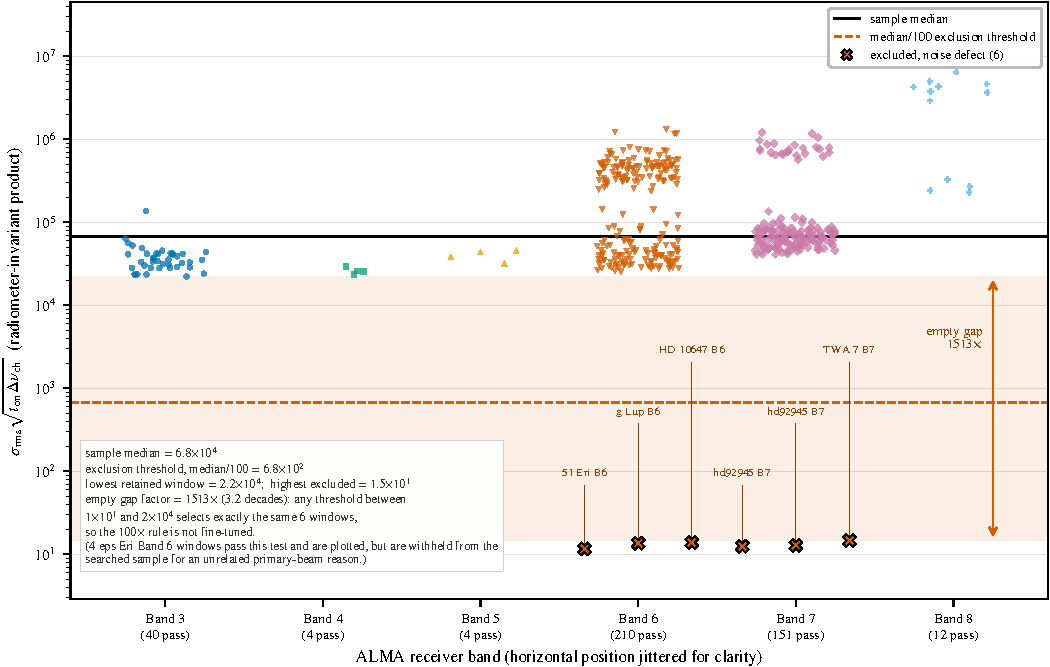
\includegraphics[width=\columnwidth]{figures/noise_qa.pdf}
\caption{Quality control on the noise estimate
(\S\ref{sec:exclusions}). The radiometer-invariant product
$\sigma\sqrt{t_{\rm on}\Delta\nu_{\rm ch}}$ varies by factors of a few
across a heterogeneous archive; the six excluded windows lie a factor
$1.5\times10^{3}$ below the lowest retained window, separated by an
empty gap.}
\label{fig:noiseqa}
\end{figure}

\subsection{Technosignature search}
\label{sec:technosearch}

All 104 star/band datasets of the searched sample yielded at least
one narrowband result; the datasets that failed at the process level
are itemised in \S\ref{sec:exclusions} and are not counted among them.
They span 417 spectral-window measurements after removal of 21
duplicate rows found in the catalogue audit
(Appendix~\ref{app:table}). The EIRP$_{5\sigma}$ limits span
$1.6\times10^{13}$--$2.8\times10^{17}$\,W, median
$1.3\times10^{15}$\,W (Figures~\ref{fig:eirp}, \ref{fig:waterfall} and
\ref{fig:context}). As expected for a volume-ordered survey, the
deepest limits are for the nearest systems ($1.6\times10^{13}$\,W for
the UV~Ceti pair at 2.7\,pc); the shallowest is $\eta$~Corvi, the
first Band~8 target searched, where distance, coarse channels, and
receiver performance set the survey's current ceiling. Against the
benchmarks of \S\ref{sec:benchmarks}, only targets within
$\sim$3\,pc reach below the Arecibo-like planetary-radar EIRP, and
none approaches the $\sim4\times10^{9}$\,W of unintentional Earth
leakage.

Four windows contain a \emph{spatially significant hit}. None
survives vetting, so this release reports \emph{zero candidates}:
Table~\ref{tab:funnel} follows the decision cascade and
Table~\ref{tab:flagged} gives each flagged window and the evidence
that dispositioned it.

\begin{table}
\centering
\small
\caption{The narrowband decision cascade of this release. Counts are
for the 417 searched windows after quality control
(\S\ref{sec:exclusions}); the vocabulary is that of
Table~\ref{tab:nomenclature}.}
\label{tab:funnel}
\begin{tabular}{@{}lr@{}}
\hline
Stage & Count \\
\hline
Channel $\times$ drift trial cells (all windows) & $3.97\times10^{7}$ \\
Control positions compared per window & 512 \\
Windows searched after quality control & 417 \\
Windows containing $\geq$1 hit ($\geq5\sigma$ at the stellar position) & 18 \\
Windows containing a spatially significant hit & 4 \\
\quad attributed to circumstellar or foreground CO & 3 \\
\quad indistinguishable from the control ensemble & 1 \\
Candidates (surviving every veto) & 0 \\
\hline
\end{tabular}
\end{table}

\begin{table}
\centering
\small
\setlength{\tabcolsep}{4pt}
\caption{The four windows containing a spatially significant hit, and
the evidence that dispositioned each. $T_\star$ is the search statistic
at the stellar position (Eq.~\ref{eq:tstar}) and `ring max' the largest
of the 512 control statistics of the same window; $p$ is the add-one
rank probability, whose floor is $1/513=0.0019$. The velocity offset is
topocentric, from the nearest catalogued transition of the eight masked
species; the $\pm50$\,km\,s$^{-1}$ mask is applied in the stellar frame
after the conversion chain of Appendix~\ref{app:conventions}. No
disposition rests on a single test.}
\label{tab:flagged}
\begin{tabular}{@{}llrrrl@{}}
\toprule
Window & $\nu$ (GHz) & $T_\star$ & ring max & $\Delta v$ (km\,s$^{-1}$) & Disposition \\
\midrule
$\beta$~Pic B3 & 115.2605 & 14.65 & 7.27 & $-26.9$ (CO $1{\to}0$) & circumstellar CO \\
$\beta$~Pic B6 & 230.5164 & 11.68 & 9.12 & $-28.4$ (CO $2{\to}1$) & circumstellar CO \\
HD~48370 B6 & 230.7305 & 27.10 & 26.83 & $-34.2$ (CO $2{\to}1$) & CO cloud emission \\
CP$-$72~2713 B7 & 345.1152 & 5.81 & 5.68 & $-1326$ (CO $3{\to}2$) & control-ensemble background \\
\bottomrule
\end{tabular}
\end{table}

Two questions are kept separate: whether four spatially significant
hits is more than this survey's own calibration predicts (a counting
question), and whether any individual hit is distinguishable from the
empirical background or from known astrophysical emission (the
dispositions below). The answers are no and no.

\subsubsection*{Survey-level false-alarm calibration}

Each window-level test compares the peak signal-to-noise ratio at the
star's position with the same statistic at 512 control positions.
Because the drift-rate grid and the thousands of channels are applied
identically to star and controls, this calibration absorbs the
per-window trials factor empirically. From this version the statistic
is \emph{symmetric}: the on-source quantity is the single propagated
stellar position, exactly what each control contributes. Earlier
versions maximised it over a small region centred on that position
while each control remained a single position, and that asymmetry was
not benign. Under a pure-noise null with exchangeable positions the
maximum of $n_{\rm src}$ source-region positions exceeds that of
$n_{\rm ctrl}$ single controls with probability
$n_{\rm src}/(n_{\rm src}+n_{\rm ctrl})$, which for the
$n_{\rm src}=135$ region and 512 controls of a representative window
is 21 per cent; the measured region-max star-beats-ring rate, 64 of
417 windows (15.3 per cent; Wilson 95 per cent interval 12.2--19.1),
is of that order. The symmetric statistic instead gives
star-beats-ring in 5 of 417 windows (1.2 per cent; Wilson interval
0.5--2.8), consistent with the exchangeable expectation
$1/513=0.19$ per cent per window inflated by the real maps' heavy
tails, and stable against the rate measured on the $\le$20\,pc
subsample alone. The exchangeability rate is thus the operative one,
and the survey-level false-alarm expectation follows from it directly
rather than through the bookkeeping ladder the asymmetry previously
required.

A candidate is gated by the joint criterion, whose threshold leg
dominates the rate: only 18 of 417 windows contain any $\geq5\sigma$
crossing at the stellar position. Each window contributes at most the
exchangeable rate $1/(1+n_{\rm ctrl})=1/513$, so the pure-noise null
predicts $417/513=0.81$ flags. Four flagged windows is more than that
budget alone would produce ($P(\geq4\,|\,0.81)=0.9$ per cent), which
is the correct reading rather than a tension: three of the four are
identified astrophysical emission and were never chance events. What
the chance budget must explain is the residual -- one unattributed
crossing against 0.78 expected across the 402 non-$\beta$~Pictoris
windows, the order of the expectation. This is the operative survey-level false-alarm
estimate; it absorbs execution-block systematics into the fixed block
margins and assumes only that, within a block, crossing status is
exchangeable with star-beats-ring status. Secondary bookkeeping models
span 1.0--9.2 per cent (Appendix~\ref{app:falsealarm}); the dominant
residual uncertainty is the star-beats-ring rate itself (Wilson 95 per
cent interval 12.2--19.1 per cent), giving a 4--19 per cent bracket on
$P(F\geq3)$.

One ensemble limit follows. With 512 controls the smallest resolvable
per-window $p$-value is $1/513$, so a Bonferroni threshold over 417 windows ($1.1\times10^{-4}$) lies below what the controls can
measure. They can show a crossing to be unremarkable but cannot
certify one as significant survey-wide; that burden falls on
localisation, recurrence, and astrophysical attribution, which decide
each flag below. We state the consequence for the planned sequence of
releases now rather than after the fact. Each release of $N$ windows
contributes ${\sim}N/513$ chance flags, so a programme reaching the
full ${\sim}2000$-window census expects ${\sim}4$: reporting one
unattributed marginal crossing per release is the \emph{expected}
outcome, not an accumulating anomaly. We therefore pre-commit to the
criterion that no crossing will be advanced as a candidate on rank
statistics alone at any point in this programme. Promotion requires
evidence the control ensemble cannot supply -- recurrence at an
independent epoch, or a control ensemble enlarged for that window
until the rank probability can resolve a survey-wide significance
($\gtrsim10^{4}$ positions for a Bonferroni threshold over the
completed census; \S\ref{sec:futurework}). Until then every such
crossing is reported, dispositioned as consistent with chance, and
released with its products. No model in the bracket promotes any
flagged window to a candidate: the three CO dispositions rest on
kinematic attribution to emission that is resolved, mapped, or
independently published, and the CP$-$72~2713 standing is a rank
statement invariant to the bookkeeping model.

\emph{Is the ring exchangeable with the star?} The $1/513$ expectation holds only if the star and its 512 controls
are exchangeable under the null, which spatially varying noise,
sidelobes, correlated pixels or phase-centre-localised calibration
residuals could each spoil. We measure it by stratum
(Fig.~\ref{fig:ctrldiag}). The median per-window control maximum is
flat across receiver bands -- 4.46, 4.59, 4.42, 4.52, 4.63 and 4.69 in
Bands 3 to 8 -- and a Kolmogorov--Smirnov test of the per-window rank
of the star among its own controls against $U(0,1)$ is consistent in
every band ($p=0.14$--0.83) and for the coarse-channel stratum
($p=0.71$). Fine-channel windows sit systematically higher in the
statistic (control maximum 5.76 against 4.42), which is expected from
their far larger channel$\times$drift trial count and is not itself a
violation, because the test is conditional on the window.

One stratum does depart, and we report it rather than pool it away:
the fine-channel windows fail the same $U(0,1)$ test at $p=0.018$
($n=111$), and contain four windows whose on-star peak exceeds their
own control maximum against 0.22 expected. Those four are precisely
the four flagged windows of Table~\ref{tab:flagged}. The departure is
therefore astrophysical signal concentrated in the windows with the
finest channels, where real narrow lines are detectable, rather than
evidence that the control ring misbehaves; but it is a genuine
stratum-level departure from exchangeability, and a reader should
treat fine-window rank probabilities as slightly optimistic. Two
stratifications cannot be made from the retained products, which store
no per-control radial position or primary-beam gain: the ring sits at
a radius small compared with the primary beam (targets lie a median
$0.1$\,arcsec from the pointing centre), so all controls share the
target's beam response by construction, but we have not measured that
and say so. The remaining robustness checks -- the trials-count
reconciliation under channel adjacency and the control-ring geometry
-- are in Appendix~\ref{app:falsealarm}.

\begin{figure}
\centering
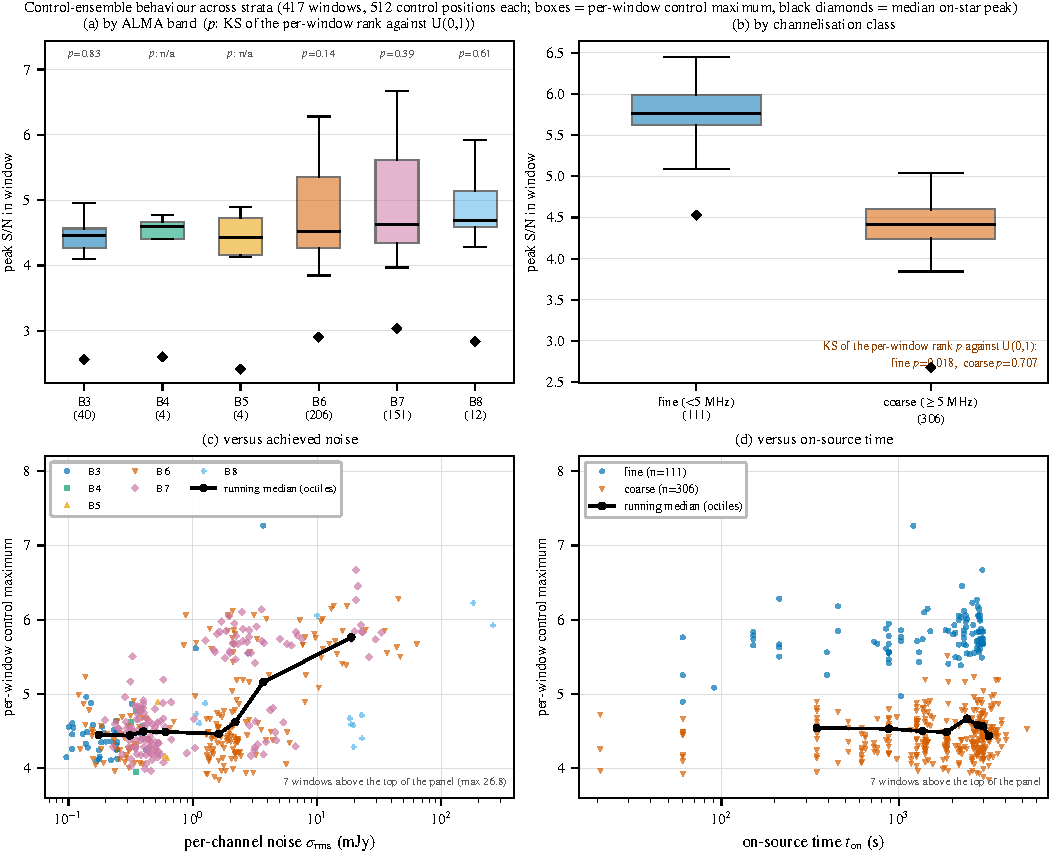
\includegraphics[width=\columnwidth]{figures/control_diagnostics.pdf}
\caption{Exchangeability of the 512-position control ring, by stratum.
Boxes give the per-window control maximum, diamonds the median on-star
peak, and $p$ the Kolmogorov--Smirnov test described in the text. The
ensemble tracks the on-star statistic in every band and at both
channelisations; the fine-channel stratum is the one departure
($p=0.018$), driven by the four flagged windows of
Table~\ref{tab:flagged}.}
\label{fig:ctrldiag}
\end{figure}

\subsubsection*{The symmetric star-versus-control null}

The survey's designed principal test applies the identical
source-region, drift-rate, and frequency maximisation at the star's
position and at every one of the 512 control locations under a single
search rule. That requirement cannot be met from the frozen release
products, so its domain is the seven locally reprocessed windows --
the six validation windows and the AU~Mic candidate's first-epoch
block -- all of which give $T_\star=3.7$--$4.9$ against control maxima
of 6.7--7.7, $p=0.81$--1.00 (Figure~\ref{fig:symcdf}, online-only
appendix): the star position is statistically exchangeable with its
control ring wherever the test can be run at full symmetry.
Extending it to all 417 windows requires per-window raw-visibility
reprocessing that the retained products do not support, so the
empirical star-versus-ring calibration above remains the operative
release-wide estimate and the symmetric statistic a validation subset.
The machinery ships with the release; the full statement, with the
consolidated family-wise trials factors of Table~\ref{tab:trials}, is
in Appendix~\ref{app:falsealarm}.

\subsubsection*{Dispositions of the four flagged windows}

Two of the four are towards $\beta$~Pictoris, a
debris-disc system with previously reported CO emission
\citep{Matra2017}: one in Band~3 at 115.2606\,GHz, 10.56\,MHz below
the CO($J{=}1{\to}0$) rest frequency, the other in Band~6 at
230.5161\,GHz, 21.87\,MHz below CO($J{=}2{\to}1$). Neither
coincidence is exact, so the automated line check did not catch them.
Carried through the full frame chain (Table~\ref{tab:bpicaudit};
Fig.~\ref{fig:bpicvel}), the offsets correspond to the same kinematic
component -- $-2.7$ and $-3.5$\,km\,s$^{-1}$ from stellar systemic,
0.74\,km\,s$^{-1}$ apart -- in the two lowest CO rotational
transitions of a system with directly detected circumstellar CO; the
coarse Band~6 window without a candidate, from a third epoch six
years earlier, independently shows CO at $-3.6$\,km\,s$^{-1}$ in the
same frame. All three epochs and both transitions land within
$0.9$\,km\,s$^{-1}$ of each other and $3.6$\,km\,s$^{-1}$ of
systemic, deep inside the $\pm50$\,km\,s$^{-1}$ mask. The frame chain
matters: the raw topocentric offsets are $-27.5$ and
$-28.4$\,km\,s$^{-1}$. We attribute both to this kinematically offset
CO emission.

Their empirical significance under the release background is
nonetheless extreme, so the attribution should not be mistaken for
dismissal: the Band~3 region peak of 20.3 exceeds all 417 per-window
control maxima (add-one $p<0.0044$), and the Band~6 peak of 12.8
exceeds all but one -- that window's own CO-filled control ring, which
reaches 15.2, by far the highest control maximum of the release
($p\approx0.0088$). Standing out this sharply is why they demanded
astrophysical attribution rather than summary rejection as noise. That
attribution came from inspecting the offsets against known CO
kinematics, not from the automated chain, which did not catch them;
the alternative would require a transmitter placed coincidentally at
matched offsets from two CO transitions in the same star.

The third, towards HD~48370 in Band~6, is the largest excess in the
release in absolute terms and the smallest in relative terms:
$T_\star=27.10$ against a control-ring maximum of 26.83, so the star
exceeds its ring by one per cent of the statistic. That signature --
star and controls rising together -- is what emission filling the
primary beam looks like, and the window sits $-34.2$\,km\,s$^{-1}$
topocentric from CO($J{=}2{\to}1$). The attribution is independently
published: \citet{Cataldi2023} report prominent CO($2{\to}1$) and
$^{13}$CO($2{\to}1$) emission towards HD~48370 at
$v_{\rm bary}\approx41$\,km\,s$^{-1}$, well separated from that
system's $23.6$\,km\,s$^{-1}$ systemic velocity and attributed by them
to foreground cloud contamination; our window recovers that feature.
The case is also a stated limitation of the spatial test: what
identifies this window is the velocity coincidence and the
near-equality of star and ring, not the rank statistic.

The fourth, towards CP$-$72~2713 in Band~7, is the only flagged window
with no astrophysical attribution, and it is marginal.
$T_\star=5.81$ against a ring maximum of 5.68: it beats its ring by
0.13 and therefore attains only the rank-probability floor,
$p=1/513$, which is the smallest value 512 controls can express and
not a measurement of significance. The margin is smaller than the scatter of the same statistic across
this star's own windows, whose other fine-channel control maxima are
5.16, 5.41, 5.67 and 5.85: 5.81 is a value its control ensembles reach
routinely in windows where the star does not cross threshold. The nearest transition of the eight masked
species lies 1326\,km\,s$^{-1}$ away; since that mask is a
contamination cut rather than a claim of completeness over the
mm/submm line forest, we re-queried the window against a wider
catalogue, whose closest entry is H$^{13}$CN($J{=}4{\to}3$) at
$-195$\,km\,s$^{-1}$, still far outside any circumstellar tolerance.
No line attribution is available. The archive holds a single execution
block covering this frequency, so no second-epoch recurrence test is
possible. We report it as a marginal
crossing consistent with the 0.81 flags expected by chance across the
release, attach no technosignature interpretation to it, and note that
a recurrence observation is the one measurement that would settle it.

\begin{figure}

\includegraphics[width=\columnwidth]{figures/bpic_velocity_space.pdf}
\caption{Stellar-frame velocity offsets of the candidate windows,
carried through the full frame chain (topocentric $\rightarrow$
barycentric $\rightarrow$ stellar; Table~\ref{tab:bpicaudit}).
Shaded band: the $\pm50$\,km\,s$^{-1}$ molecular-line exclusion mask.
\emph{Top:} the two $\beta$~Pictoris candidates fall well inside the
mask as a single kinematic component, resolved in the inset. \emph{Bottom:} the flagged window towards CP$-$72~2713, and the
AU~Mic crossing that the symmetric statistic does not flag
(\S\ref{sec:aumic}), sit far outside any circumstellar tolerance and
are dispositioned by their spatial behaviour, not by the mask.}
\label{fig:bpicvel}
\end{figure}

\begin{table*}
\centering
\small
\caption{Line-attribution audit of the three candidate windows
(first three rows) and the coarse $\beta$~Pictoris Band~6 window
without a candidate
that independently shows the same CO component, carried through the
frame chain of \S\ref{sec:frames}. Topocentric offsets are observed
minus catalogued rest frequency (CO $J{=}1{\to}0$ 115.271202\,GHz,
CO $J{=}2{\to}1$ 230.538000\,GHz, \citealt{Pickett1998}). The
barycentric correction is the Earth-ephemeris term at the
execution-block mid-time (block uids in Table~\ref{tab:ebs}); the
systemic radial velocities are the catalogued values (SIMBAD;
\emph{Gaia} DR3 for $\beta$~Pictoris, \citealt{GaiaDR3}; \emph{Gaia}
DR2 for AU~Mic, \citealt{Fouque2018}).}
\label{tab:bpicaudit}
\begin{tabular}{@{}llrrrrrr@{}}
\toprule
Flag & UTC start & $f_{\rm obs}$ (GHz) &
Transition & Topo.\ offset & Bary.\ corr. & $v_{\rm sys}$ &
Stellar-frame \\
 & & & & (MHz; km\,s$^{-1}$) & (km\,s$^{-1}$) & (km\,s$^{-1}$) &
offset (km\,s$^{-1}$) \\
\midrule
$\beta$~Pic B3 & 2022-03-02 23:14 & 115.260644 &
CO($1{\to}0$) & $-10.56$; $-27.46$ & $-7.90$ & $+16.84$ & $-2.72$ \\
$\beta$~Pic B6 & 2019-03-12 00:14 & 230.516128 &
CO($2{\to}1$) & $-21.87$; $-28.44$ & $-8.15$ & $+16.84$ & $-3.45$ \\
AU~Mic B6 & 2014-08-18 04:01 & 230.825230 &
CO($2{\to}1$) & $+287.23$; $+373.51$ & $-10.02$ & $-4.71$ & $+378.82$ \\
$\beta$~Pic B6$^{\dagger}$ & 2013-10-06 06:23 & 230.528134 &
CO($2{\to}1$) & $-9.87$; $-12.83$ & $+7.63$ & $+16.84$ & $-3.62$ \\
\bottomrule
\end{tabular}
\parbox{\textwidth}{\footnotesize $^{\dagger}$Coarse
Band~6 window without a candidate (Appendix~\ref{app:table}); shown
because it independently exhibits the same CO component as the
candidate fine window of the same band.}
\end{table*}

\subsubsection*{Line exclusion: definition, cost, and limits}

The searches ran with an automated line check matching a crossing
against catalogued rest frequencies within one spectral channel at
zero drift. The $\beta$~Pictoris candidates showed that check
inadequate: both fell outside its one-channel tolerance (by 10.6 and
21.9\,MHz) while corresponding, after the frame chain, to a kinematic
component within 3.6\,km\,s$^{-1}$ of stellar systemic of a resolved,
previously mapped disc -- exactly the regime a channel-width tolerance
is blind to. Before publication every crossing was reclassified with a
velocity-space mask ($\pm50$\,km\,s$^{-1}$ in the stellar frame around
each catalogued transition), which is the published pipeline's
line-exclusion definition from this release onward. Its kinematic
justification, its empirical conservatism, the retrospective
reclassification of every crossing, and the ``Schelling point''
counter-argument that a deliberate communicator might choose exactly
these frequencies are set out in Appendix~\ref{app:linemask}; applied
retrospectively the mask rejects exactly the two $\beta$~Pictoris
candidates and changes no other disposition.


The masking cost is stated on one definition throughout: every JPL
catalogued transition of the eight species (276 transitions),
displaced by each system's radial velocity, $\pm50$\,km\,s$^{-1}$
stellar-frame half-width, intersected with each window and merged.
The release effectively searches 87.0\,GHz of unique sky frequency --
the disjoint union of the searched windows minus the part of the mask
inside it (Figure~\ref{fig:waterfall}) -- down from 92.4\,GHz before
masking, a 5.7 per cent reduction. Summed over the 417 windows the
mask removes 41.4\,GHz of the 700.8\,GHz of gross window bandwidth
(5.9 per cent; per-species, per-band breakdown in
Table~\ref{tab:maskband}, online-only appendix), and the per-window
usable fraction has median 0.960 (10th percentile 0.790). Union
bandwidth is exposure-blind, a window visited for seconds counting the
same as one integrated for an hour, so we also report the summed
per-star frequency union, 371.9\,GHz, and the summed product of
on-source time and searched bandwidth, $1.4\times10^{6}$\,s\,GHz
(per-window on-source time spans 12.1--5274\,s, median 2570\,s).
Because the mask governs dispositions and not the noise-derived
thresholds, the quoted EIRP$_{5\sigma}$ values are unchanged; no
signal was found outside the excluded velocity regions in any window.

The mask is thus a selection effect of the survey's design, and the
distinction matters for how a masked crossing should be described: a
signal coincident with a molecular line is not thereby ``false'', it
is \emph{excluded from the technosignature search domain} because the
astrophysical prior there is overwhelming and this pipeline cannot
separate the two. No constraint is placed on transmitters within the
excluded regions -- 5.9 per cent of the searched bandwidth -- and a
search for deliberately line-adjacent carriers would need a
complementary strategy. The exposure is not limited to the candidate
windows: 131 of 417 windows (58 per cent) contain a catalogued
transition of the eight species in-band, and all four spatially significant
windows do, yet in none does a crossing fall within one native channel
of a rest frequency -- precisely the regime the velocity-space
criterion covers.

\subsection{Changing the detection statistic, and the AU~Mic crossing}
\label{sec:aumic}

An initial implementation of the search maximised the statistic over a
$n_{\rm src}=135$-position region centred on the star while comparing
it against 512 \emph{single}-position controls. A crossing towards
AU~Mic in Band~6 at 230.83\,GHz was identified under that statistic
and was carried as a candidate. Because a criterion revised after
inspecting the object it must judge is a criterion a reader is
entitled to distrust, we set out the sequence and the evidence
explicitly.

The defect is a property of the statistic, demonstrable without
reference to any target: the region-max asymmetry raises the
star-beats-ring probability under a pure-noise null to 20.9 per cent
(\S\ref{sec:technosearch}) against $1/513=0.19$ per cent for a
symmetric test, and the measured release-wide region-max rate, 15.3
per cent, is of exactly that order. That calculation, and the
release-wide rate that confirms it, involve no candidate. We
therefore replaced the statistic with the symmetric single-position
form of Eq.~\ref{eq:tstar}, applied identically to the star and to
every control, and re-ran the whole release under it.

The change is a bias correction, not a loss of sensitivity, and this
is checkable rather than assertable. Across the 417 searched windows
the set flagged by the symmetric criterion is a strict \emph{subset}
of the set flagged by the region-max criterion: seven windows were
flagged before, four are flagged now, and the three that dropped out
(towards ALMA~J1537$-$3319, AU~Mic and HD~14055) have in common that
the \emph{stellar position itself never exceeded its own control
ring} -- star statistics of 5.09, 5.22 and 5.22 against ring maxima
of 5.63, 5.85 and 5.74. The symmetric criterion removed no window in which the star dominated
its controls -- the only configuration a localised transmitter can
produce, since a real point source at the stellar position raises
$T_\star$, the quantity the new test uses. Consistently, the
injection campaign recovers signals through the unmodified pipeline on
the star position (\S\ref{sec:ancillary}), so its measured
completeness is a property of the symmetric statistic as reported.

Under the symmetric criterion the AU~Mic crossing is not flagged: 10
of its own 512 controls reach or exceed the stellar statistic, an
empirical $p=0.021$ far from the $1/513$ floor. It also fails two
direct, pre-named tests -- it is not localised at the stellar
position, and it does not recur at a second epoch
(Table~\ref{tab:aumic}).

\begin{table}
\centering
\small
\setlength{\tabcolsep}{4pt}
\caption{The AU~Mic candidate frequency (230.8252\,GHz) under the
three treatments that decide it: the release's frozen products
(region-max statistic), the fully symmetric reprocessing of the same
first-epoch execution block (2014 August~18; observatory calibration
recipe applied verbatim), and the second-epoch block of the same
programme (2014 June~5; identical search treatment).}
\label{tab:aumic}
\begin{tabular}{@{}lrrr@{}}
\toprule
 & Release & Symmetric & Second epoch \\
Statistic & (region-max) & reprocess. & (recurrence) \\
\midrule
Star statistic & 5.97 & 4.93 & 4.77 \\
Control maximum (512) & 5.85 & 7.70 & 6.78 \\
Star rank $p$ (add-one) & --- & 0.81 & 0.97 \\
Single-position star statistic & 5.22 & --- & --- \\
Per-channel S/N (zero drift) & --- & 2.46 & 2.22 \\
Peak drift (Hz\,s$^{-1}$) & 1418.5 & 1593 & 1281 \\
\bottomrule
\end{tabular}
\end{table}

Localisation, recurrence, and statistical scale are reported in full
in Appendix~\ref{app:aumic}, with the numbers of
Table~\ref{tab:aumic}. Neither the reprocessed first epoch nor the
one further public Band~6 block covering 230.83\,GHz shows a
localised excess at the stellar position, and that second epoch is a
clean non-recurrence -- which rejects a continuous or repeating source
at this frequency and these epochs without constraining intermittent
transmission.

The archival epochs also bound what this release can say about duty
cycle: each star was observed in one to three execution blocks,
searched independently with no epoch stacking, so the non-detection
concerns the archival epochs observed, not permanent activity. The surplus of available over searched execution blocks
(\S\ref{sec:discussion}) is the recurrence pool the second-epoch test
drew on, and \S\ref{sec:discussion} turns the epoch structure into an
explicit duty-cycle constraint.
\subsection{Ancillary results}
\label{sec:ancillaryresults}

Three ancillary results are reported in full online.

\emph{Integration-time audit} (Appendix~\ref{app:audit}). The
on-source integrations quoted here were reconstructed from pipeline
bookkeeping rather than retained natively, so all 227 window-level
records were audited against the ALMA archive's own exposure
accounting. Two of the 58 star--execution-block groups over-count --
AT~Mic by a factor 1.43, an internally diagnostic dump-bookkeeping
artefact already corrected to the archive's 877\,s in
Table~\ref{tab:duty}, and CD$-$38~10980 by 7 per cent -- and the rest
are conservative. No EIRP
threshold depends on the audited quantity, since thresholds derive
from the measured per-channel rms rather than from integration time;
the audit is conservative for every window of both candidate hosts, so
no disposition changes; and the exposure-weighted coverage figure of
\S\ref{sec:technosearch} is at worst optimistic by less than 1 per
cent. The defect class this audit caught was found by chance in one
target, which is why a direct per-execution-block export is committed
for the next release.

\emph{Continuum search} (Appendix~\ref{app:contsearch}). The
continuum lane has been run over the 57 target/bands processed far
enough to carry a usable continuum measurement -- a subset of the
narrowband sample, and the one place in this paper where a count
refers to fewer than the 417 searched windows. Seventeen show a
$\geq5\sigma$ detection and forty are non-detections reaching
0.036--3.6\,mJy (median 0.52\,mJy); every detection is
astrophysically unsurprising, the auroral emitter LSR~J1835$+$3259
meriting deeper follow-up. The lane is exploratory, its statistical power is unquantified at this
depth, and no technosignature disposition in this paper rests on it.

\emph{Serendipitous molecular-line catalogue}
(Appendix~\ref{app:linecat}). The line-exclusion step identifies every
$\geq5\sigma$ outlier channel as a byproduct. Across the subset
scanned, 18 outlier groups were found, of which six are plausibly
real. All are reported openly, including the two we consider probably
spurious.

\begin{figure}
\centering
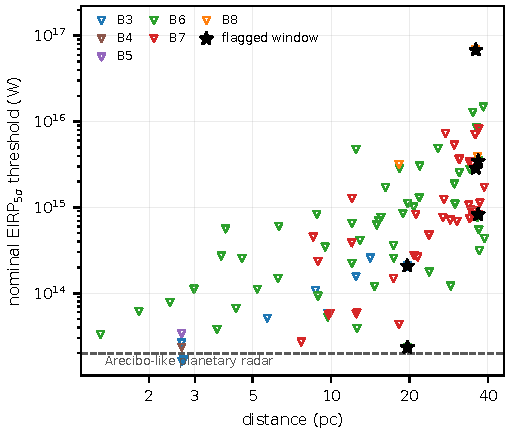
\includegraphics[width=\columnwidth]{figures/eirp_vs_distance.pdf}
\caption{Nominal EIRP$_{5\sigma}$ thresholds against distance, one
deepest window per star and band (104 datasets, 85 stars); every point
is an upper limit. Stars mark the four windows containing a spatially
significant hit (Table~\ref{tab:flagged}). The dashed line is the EIRP
of an Arecibo-like planetary radar, $2\times10^{13}$\,W, used purely
as a scale for human transmitter power and not as a claim that the
survey reaches Earth-technology detectability
(\S\ref{sec:benchmarks}). Thresholds are nominal in the sense of the
boxed rule of \S\ref{sec:method}.}
\label{fig:eirp}
\end{figure}



\begin{figure*}
\centering
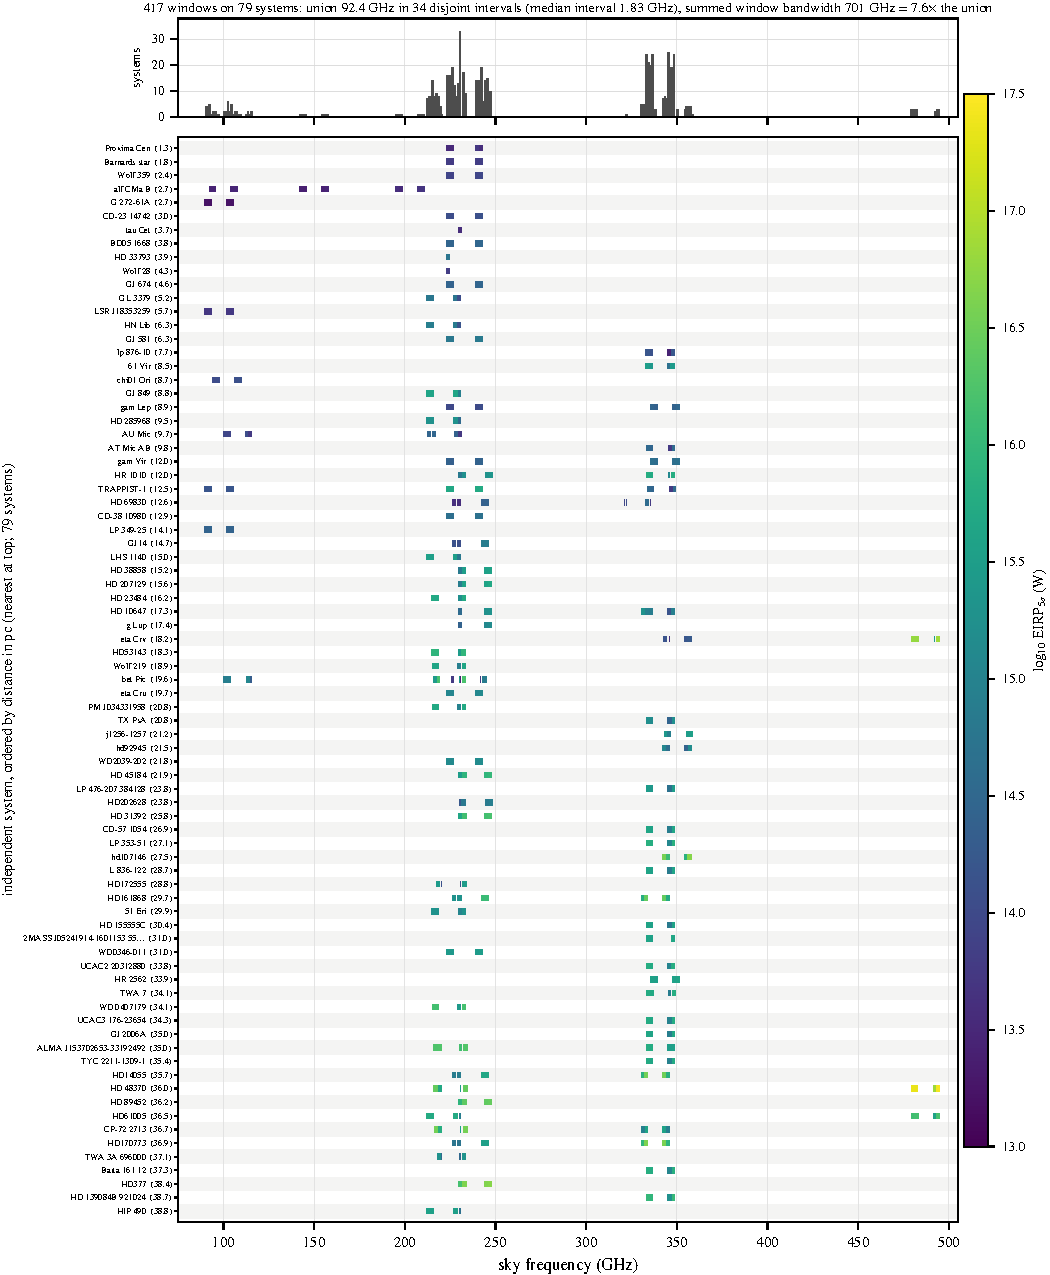
\includegraphics[width=0.82\textwidth]{figures/coverage_waterfall.pdf}
\caption{What this survey actually sampled in frequency. Each searched
spectral window is drawn as a horizontal segment on the row of its
host system, rows ordered by distance, coloured by that window's
nominal EIRP$_{5\sigma}$ threshold; the upper panel counts systems
covering each gigahertz of sky frequency. The 92.4\,GHz frequency
union is assembled from 34 disjoint islands of median width
1.8\,GHz, concentrated near 230 and 345\,GHz, and the summed window
bandwidth exceeds the union by a factor 7.6 -- the coverage is
narrow, clustered and repeatedly revisited, not broad. These are the
intervals on which the occurrence limits of \S\ref{sec:discussion}
are conditioned. Thresholds are nominal in the sense of
\S\ref{sec:method}.}
\label{fig:waterfall}
\end{figure*}



\section{Discussion}
\label{sec:discussion}
This paper is the survey's first stand-alone processed release, and
its results are preliminary by construction: 104 of 208 planned
target/bands ($\sim$41 per cent) are complete, and the processed
subset is sensitivity-ranked -- nearest, most sensitively-constrained
systems first -- so it is not an unbiased draw, and the full sample
will extend these results to larger distances and shallower faint-end
limits. No credible technosignature has been
found, and the quoted EIRP$_{5\sigma}$ thresholds of
Appendix~\ref{app:table} bound any transmitter present above them. Two candidates towards $\beta$\,Pic are attributable to
CO disc emission -- underlining, as \citet{Mason2024} highlight, the
importance of checking any mm-band narrowband crossing against known
molecular transitions; that check is automated for every crossing
(\S\ref{sec:method}) and now uses a velocity-space match applied
retroactively to every window (\S\ref{sec:technosearch}). The third,
marginal candidate (AU~Mic, \S\ref{sec:aumic}) is not statistically
distinguishable from the empirical background and remains recorded
for future re-examination rather than dismissed.

The scale of the space searched is stated on one definition
throughout in \S\ref{sec:technosearch} and
Figure~\ref{fig:waterfall}. For context on the drift ceiling, of the
37 planets known around the 15 planet-hosting targets only
TRAPPIST-1\,b, in its edge-on worst case at
$\sim$13\,Hz\,s$^{-1}$\,GHz$^{-1}$, reaches it; GJ~581\,e,
61~Vir\,b, and TRAPPIST-1\,c reach roughly half of it, and the
remaining 33 planets all sit well inside the searched
grid.\footnote{Star--planet relative accelerations $GM_\star/r^{2}$
from NASA Exoplanet Archive planetary-companion parameters (Mission
Star/Planet table, accessed 2026 September), maximised over orbital
phase and inclination.}

Table~\ref{tab:searchspace} (\S\ref{sec:results}) consolidates the
axes along which a transmitter is or is not detectable, and
Table~\ref{tab:perband} (online-only appendix) decomposes the same
release by ALMA band.




Coverage eligibility and search completeness are different
quantities. The census of public usable ALMA data
(\S\ref{sec:sample}) establishes eligibility, and every held execution
block within this release's scope was searched, so no EB-level
selection lies behind the 57. Availability is
measured directly rather than inherited from the release bookkeeping:
a proper-motion-matched census of the ALMA archive (2026
September~9; public rows, all bands, pointing within 30\,arcsec of
the propagated stellar position at the observation epoch) counts 107 unique public on-star EBs over the subset on which it has
been run, and re-finds all but one of that subset's searched EBs (the exception, TRAPPIST-1's Band~7 execution
A002/Xcccc19/X5564, is carried by \texttt{obscore} only through its
calibrator-field row -- an archive-representation artefact biasing
the census low by one for that star). The full selection
funnel, from archive availability to the zero-candidate outcome, is
Figure~\ref{fig:selection} (online-only appendix), and the
machine-readable ledger \texttt{v323\_star\_coverage.json} gives
per-star distance, availability, scope, and searched frequency
intervals.

Figure~\ref{fig:accel} (online-only appendix) shows the drift ceiling
as an explicit selection function over planet period and host mass,
and its cost is stated plainly: a transmitter bound to any known
planet in the sample other than the innermost TRAPPIST-1 planets
would produce drift rates the search covers in full; one whose drift exceeds the ceiling is outside the searched grid and
sacrificed by design (Appendix~\ref{app:extended} recovers some
non-linear morphologies). The host-mass dependence is weak
($a \propto M_\star^{1/3}$ at fixed period), so the ceiling is
effectively a function of orbital period alone; and the calculation
constrains only transmitters co-located with \emph{known} planets --
one on an undiscovered planet, or on a platform with accelerations of
its own choosing, is covered only in so far as its drift falls within
the searched grid.

Placing the release against the published haystack of
\citet{Wright2018} is likewise best done axis by axis. On their
frequency axis (10\,MHz--115\,GHz), only the Band~3 portion of our
union lies inside their boundaries (20.6\,GHz of 115\,GHz, or 0.18 of
the axis, and a part their Hz-resolution surveys reach far more
finely); the remaining 66.6\,GHz (Bands~4--8, 125--495\,GHz) lies
entirely outside it -- the genuinely new territory of this release.
On their transmitted-bandwidth axis (0--20\,MHz), a single-channel
search of native channels probes a fraction set by the channel width
(window-mean 0.63, median 0.78). On their sensitivity axis, our
median threshold ($7.3$\,mJy across a 15.625-MHz channel, i.e.\
$\phi\approx1.1\times10^{-21}$\,W\,m$^{-2}$) detects a $10^{13}$\,W
transmitter only within ${\sim}0.9$\,pc. Against the only prior
ALMA-archival technosignature search, \citet{Mason2024} reach 28
bycatch targets at $\geq$1.01\,kpc with a deepest quoted
EIRP$_{\rm min}$ of $6.91\times10^{17}$\,W, whereas this release's 42
systems all lie inside 20\,pc at median per-target thresholds
${\sim}2500\times$ deeper: the two searches occupy nearly disjoint
corners of the same haystack, near versus deep. We do not multiply
these fractions into a combined haystack coverage -- the axes are
strongly coupled (distance and sensitivity above all), and a product
of marginal fractions would misstate the true overlap by orders of
magnitude.

\subsection{Occurrence limits}

What a zero-detection result bounds is a fully conditioned quantity.
Writing the per-system completeness as
\begin{equation}
C_i(P) = F_i\,R_i(P)\,D_i\,C_{i,\rm drift},
\label{eq:conditioning}
\end{equation}
where $F_i$ is the probability that the transmitter's sky frequency
falls inside the intervals actually searched for system $i$, $R_i(P)$
the probability that a transmitter of EIRP $P$ would have crossed
system $i$'s threshold had it been emitting there, $D_i$ the
probability that it was emitting during the analysed archival
interval, and $C_{i,\rm drift}$ the recovery probability for a carrier
of the searched drift and temporal morphology
(Appendix~\ref{app:inject}), the probability of zero credible
detections when a fraction $f$ of systems hosts a matching transmitter
is
\begin{equation}
P(N_{\rm det}=0\,|\,f)=\prod_{i=1}^{N_{\rm sys}}\left(1-f\,C_i\right),
\label{eq:prevalence}
\end{equation}
and the one-sided 95\% upper limit $f_{95}$ solves
$P(N_{\rm det}=0\,|\,f_{95})=0.05$.

\noindent\fbox{\parbox{0.96\columnwidth}{\small
\emph{Reading rule.} Among the ALMA-observed systems, fewer than
$f_{95}(P)$ per cent host a transmitter of EIRP $\geq P$ that was
emitting during the archival observations, at a sky frequency within
the particular spectral intervals searched for that system, with drift
and temporal morphology lying within the searched class.}}

\noindent \emph{What is and is not being inferred.} Setting
$F_i=D_i=1$ is not a claim that these factors are near unity. It is a
statement that the inference is \emph{conditional} on them, in the
sense of the reading rule above; Fig.~\ref{fig:waterfall} shows
exactly what set of spectral intervals the frequency condition refers
to. A reader who wants an unconditional prevalence must multiply
by their own priors on transmitter frequency and duty cycle, and those
priors, not our data, will dominate the answer.

We evaluate Eq.~\ref{eq:prevalence} on the 79 independently observed
systems (85 narrowband-searched stars; six bound pairs share
observations and are counted once each) in two forms
(Table~\ref{tab:occurrence}). The \emph{thresholded} form is the step function the retained
products support directly, $R_i(P)=1$ when system $i$'s deepest window
threshold lies below $P$ and 0 otherwise; the \emph{measured} form
integrates the injection-recovery curve of Appendix~\ref{app:inject}
over each system's searched bandwidth,
$R_i(P) = \sum_w \Delta\nu_w\, {\rm rec}(5P/{\rm
EIRP}_{5\sigma,w}) / \sum_w \Delta\nu_w$, folding in the
$17\rightarrow83$ per cent recovery of the searched class measured
between four and ten times the noise. It is defined on the 56 systems with at least one fine-channel window;
the coarse-channel-only systems have no measured recovery for the
drifting class, so the measured ladder is a 56-system bound.

\emph{Which number is the result.} The measured form is the
observational result of this paper, because it is the only one in
which the recovery fraction has been measured rather than assumed. At
EIRP $\geq10^{16}$\,W it gives $f_{95}=6.5$ per cent. The thresholded
form (3.8 per cent) assumes unit recovery, and a uniform
$C=0.42$ assumption gives 9.0 per cent; both are bracketing
calculations and neither should be quoted as the survey's constraint.
The measured form is not simply the weakest of the three: for systems
whose fine-channel thresholds lie well below $P$ the measured recovery
rises above 0.42 towards its 0.83 plateau, which is why it falls
between the two idealisations rather than outside them. A Bayesian
treatment with a uniform prior on $f$, $p(f\,|\,{\rm
data})\propto\prod_i(1-f\,C_i)$, gives a 95 per cent credible upper
bound of 6.4 per cent for the same completeness model -- agreement to
better than the width of the last quoted digit, so nothing here turns
on the frequentist construction.

\begin{table}
\centering
\small
\setlength{\tabcolsep}{4pt}
\caption{The 95 per cent upper limit $f_{95}(P)$ on the occurrence of
transmitters above EIRP $P$, conditional on emission inside the
searched spectral windows and throughout the archival epochs. $n$ is
the number of systems with non-zero completeness at that $P$; the
\emph{measured} column is the result of this paper. `Vacuous' means no
system has non-zero completeness, so no bound exists.}
\label{tab:occurrence}
\begin{tabular}{@{}lrrrr@{}}
\toprule
$P$ (W) & \multicolumn{2}{c}{thresholded (unit $C$)} &
\multicolumn{2}{c}{measured $C$ \emph{(result)}} \\
 & $n$ & $f_{95}$ & $n$ & $f_{95}$ \\
\midrule
$3\times10^{13}$ & 4 & 52.7\% & 2 & vacuous \\
$10^{14}$ & 16 & 17.1\% & 11 & 47.1\% \\
$10^{15}$ & 57 & 5.1\% & 45 & 10.1\% \\
$10^{16}$ & 78 & 3.8\% & 56 & \textbf{6.5\%} \\
$10^{17}$ & 79 & 3.7\% & 57 & 6.2\% \\
\bottomrule
\end{tabular}
\end{table}

Three caveats bound how far these numbers can be pushed. First, even
the measured form fixes $F_i=D_i=1$ and the per-system recovery at
the configuration level: it is a frequency-integrated completeness
for the searched class, not a per-system calibration. Second, the population is heterogeneous in
threshold, so each point applies to transmitters above that $P$, not
to a single well-defined class. Third, systems are treated as
independent trials in a randomly chosen archival interval; the
frequency-integrated duty-cycle dependence is quantified below. These are, to our knowledge, the first ALMA-side numbers of their
kind, and they are not competitive prevalence constraints; removing
the remaining idealisations requires the per-system $C_i(P)$ that the
retained injection campaign supports.

The archival epoch structure converts directly into a duty-cycle
constraint. Writing $D_i$ for the probability that a transmitter with
duty cycle $D$ was emitting during system $i$'s analysed intervals
($D_i=D$ to the accuracy the epoch structure supports;
Table~\ref{tab:duty} gives per-star epochs and integrations), the
same product form gives the $f_{95}(D)$ ladder of
Table~\ref{tab:f95duty} and Figure~\ref{fig:occduty}: for continuous
emitters the limits are those of Table~\ref{tab:occurrence}; at
$D=0.5$ the measured-form limit degrades from 6.5 to 13.0 per cent;
by $D=0.1$ it is 65 per cent and carries essentially no information;
and below that no bound of this form exists at all -- transmitters
active in a small fraction of randomly chosen intervals are not
constrained by single-epoch archival coverage, and only the
recurrence-pool reprocessing of future releases can touch them. Since
an intermittent transmitter is at least as plausible \emph{a priori}
as a continuous one, the $D=1$ numbers should never be quoted without
this dependence attached; the non-recurrence logic of
\S\ref{sec:aumic} points the same way.

\begin{table}
\centering
\small
\caption{Duty-cycle dependence of the 95 per cent upper limit at
$P\geq10^{16}$\,W, from Eq.~\ref{eq:prevalence} with $D_i=D$:
thresholded form (79 systems, unit recovery) and the
measured-completeness form (56 fine-calibrated systems) that is this
paper's result. `Vacuous' means no system retains non-zero
completeness and no bound exists.}
\label{tab:f95duty}
\begin{tabular}{@{}lrr@{}}
\toprule
Duty cycle $D$ & $f_{95}$ thresholded & $f_{95}$ measured \\
\midrule
1 (continuous) & 3.8\% & 6.5\% \\
0.5 & 7.5\% & 13.0\% \\
0.1 & 37.7\% & 65.0\% \\
0.01 & vacuous & vacuous \\
\bottomrule
\end{tabular}
\end{table}

\begin{figure}
\centering
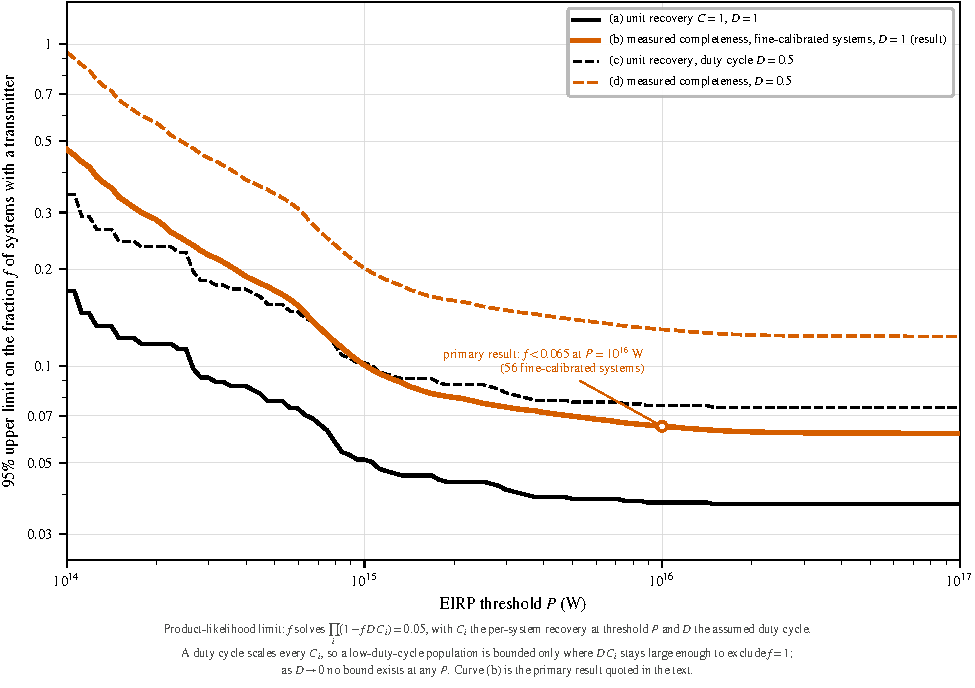
\includegraphics[width=\columnwidth]{figures/occurrence_duty.pdf}
\caption{95 per cent upper limits on the fraction $f$ of systems
hosting a transmitter above EIRP $P$, from
$\prod_i(1-f D C_i)=0.05$. Curve (b) is the result of this paper, the
injection-measured recovery integrated over each system's
fine-channel bandwidth; curves (a) and (c) assume unit recovery and
are bracketing calculations only. The shaded region is where the
surviving systems cannot exclude $f=1$ and no bound exists, and it
grows to cover every $P$ as $D\rightarrow0$.}
\label{fig:occduty}
\end{figure}

A cumulative look-elsewhere consideration accompanies multi-release
use: as releases accumulate, the probability that at least one
statistically unremarkable crossing is reported somewhere in the
programme grows toward unity even if every release is individually
clean. The guard is the procedural pre-commitment of
\S\ref{sec:technosearch}, applied per release rather than to
aggregated significance.

The data-quality exclusions of \S\ref{sec:exclusions} carry two open
engineering items, recorded here rather than buried: the
continuum-imaging step still lacks the pointing-offset guard the
narrowband step has, and the window-level noise-handling defect
affecting HD~10647 and HD~139664 is excluded from results but not yet
fixed at source. Both are corrected, and the affected datasets reprocessed, in the
single corrected public release (Data Availability). The general
lessons for archival mining are drawn together in online-only
Appendix~\ref{app:lessons}.

The four supplementary analyses of Table~\ref{tab:supp} are
infrastructure investments rather than sources of results at this
stage. Their role in the
Type-I error budget is exact: it is carried by the primary lane alone
(\S\ref{sec:technosearch}). The supplementary screens gate nothing in
that budget, are correlated with it by construction, and disposition
none of the three candidates, so their non-detections must not be
multiplied into a stronger constraint than the primary lane's own.

Because our selection is on ALMA archival coverage alone, useful
subsamples fall out without compromising the census framing, subject
to the unresolved-pair caveat of \S\ref{sec:sample}. First, 15 of the
46
processed stars (33 per cent; 36 planets) are confirmed exoplanet
hosts -- including Proxima~Centauri, $\tau$~Ceti,
$\epsilon$~Eridani, $\beta$~Pictoris, and the seven-planet TRAPPIST-1
system -- a sub-survey extractable directly from
Appendix~\ref{app:table}; HN~Lib and LHS~1140, each host to a
habitable-zone planet, now carry a genuine ALMA technosignature
non-detection alongside their planet-search literature. Second, four
of the 46 are white dwarfs (Sirius~B, Van~Maanen's Star, Wolf~219,
CD$-$38~10980), all continuum non-detections with EIRP$_{5\sigma}$
limits of $2.3\times10^{13}$--$8.4\times10^{14}$\,W -- among the very
few mm/submm SETI constraints reported for white dwarfs
\citep{PollutedWD2026}, a channel motivated by post-main-sequence
survival scenarios and the compact debris discs of metal-polluted
white dwarfs.

\subsection{Priorities for the next release}
\label{sec:futurework}

Four changes would enlarge what this experiment can say, and we rank
them by how much signal space they buy.

\emph{First, and by a wide margin: a search branch that preserves
phase-steady carriers.} The per-channel temporal-median subtraction
that suppresses stationary ground-based interference also removes a
stable narrowband beacon -- one of the canonical technosignature
morphologies -- at every amplitude we injected: not a completeness
correction, but a whole signal class the present pipeline cannot see.
An interferometer does not need median subtraction to reject
terrestrial interference: sky localisation, baseline-dependent phase,
delay and fringe-rate signatures and multi-block consistency all
discriminate a celestial source from a ground-fixed emitter without
touching its time dependence. A second branch built on them is the
highest-value change available to this survey.

\emph{Second, use the visibilities rather than extracted spectra.} A
genuine source at the star should show the geometric phase behaviour
$V_{ij}(\nu,t)=A(\nu,t)\exp[-2\pi i(u_{ij}l+v_{ij}m)]$ expected at that
sky position on every baseline. A likelihood ratio between a celestial
point source at the stellar position, a common-mode terrestrial
interferer, and image-plane noise would be strictly more powerful than ranking a peak against a control
ring. We regard this as the distinctive methodological opportunity of
ALMA SETI, available in a way it is not to single-dish or beamformed
searches.

\emph{Third, enlarge the control ensemble for interesting windows.}
The $1/513$ rank floor (\S\ref{sec:technosearch}) cannot certify
significance across a census of thousands of windows. A two-stage
scheme -- 512 controls routinely,
then $10^{4}$--$10^{5}$ local null evaluations for any window that
passes -- would let the pipeline distinguish a real candidate
statistically rather than hand every one to astrophysical vetting.

\emph{Fourth, extend the injection campaign and the polarisation
axis.} The completeness curve should be measured per band, channel width,
integration time, antenna count and primary-beam position rather than
transferred by construction, and pushed past $10\sigma$ until it
asymptotes, since it has not yet located EIRP$_{90}$. The analysis is
also Stokes~$I$ only; a polarised carrier is a physically motivated
discriminator against weakly polarised astrophysical backgrounds at
these frequencies, and polarisation-resolved reprocessing costs no
sensitivity.

\emph{A boundary worth stating precisely.} The search assumes drift is
linear over a track. Curvature matters when
$\tfrac{1}{2}\ddot\nu T^{2}$ exceeds half a native channel; for a
transmitter on a circular orbit of period $P$ this becomes
$P \lesssim 2\pi(\nu/c)\,a_{\rm max}T^{2}/\Delta\nu_{\rm ch}$, which
for a typical fine-channel window (230\,GHz, 488\,kHz channels,
$T\approx2000$\,s) is $P\lesssim1.6$\,d, and for a coarse-channel
window about an hour. Only the shortest-period orbits in the sample
reach it -- TRAPPIST-1\,b, at $1.51$\,d, sits just inside the
boundary, and is also the case that exceeds the drift ceiling. For
everything else the constant-drift model is adequate, and the
chirp-search extension (Appendix~\ref{app:extended}) is what covers
the remainder.

\medskip
\noindent\rule{\columnwidth}{0.4pt}
\smallskip
\noindent\textbf{What this survey does not constrain.}
\emph{Nothing in this paper bounds the prevalence of:}
(i) \emph{phase-steady carriers} -- a stable beacon dwelling in one
channel for more than roughly 40 per cent of a track is removed by the
per-channel temporal-median subtraction, by construction and at every
amplitude tested (\S\ref{sec:ancillary});
(ii) transmitters emitting \emph{outside the searched spectral
windows}, which are 34 narrow islands totalling 92.4\,GHz
(Fig.~\ref{fig:waterfall}), not ALMA's frequency range;
(iii) transmitters active \emph{outside the archival epochs} observed
-- the limits assume continuous emission and are already weak at duty
cycle 0.5 and vacuous below ${\sim}0.1$ (Table~\ref{tab:f95duty});
(iv) drift rates \emph{above} the searched ceiling
$|a|=3.6$\,m\,s$^{-2}$, which excludes transmitters on the most
close-in orbits, including a TRAPPIST-1\,b-like one
(Fig.~\ref{fig:accel});
(v) carriers deliberately placed \emph{inside} the
$\pm50$\,km\,s$^{-1}$ molecular-line mask, which is excluded search
space rather than searched-and-empty space;
(vi) emission substantially \emph{broader} than one native channel,
for which the quoted thresholds must be rescaled;
(vii) anything below the nominal threshold, at which measured recovery
is $42^{+16}_{-14}$ per cent, not 95 per cent.
\smallskip
\noindent\rule{\columnwidth}{0.4pt}
\medskip

\section{Conclusions}
\label{sec:conclusions}

We have described the design, methodology, and processed release of a
technosignature search of the 168 stars within 40\,pc with public
ALMA archival coverage: a complete census of ALMA-covered stars within
40\,pc, carrying no astrophysical selection of its own and with every
entry passing an independent positional and identity audit against
SIMBAD and \emph{Gaia} (\S\ref{sec:exclusions}), but covering only
${\sim}7$\% of the catalogued stars within 40\,pc and inheriting the
archive's own non-uniform targeting, so the contrast with
interest-selected samples (\S\ref{sec:sample}) is one of degree
rather than kind. This release processes 104 of the 208 planned target/bands -- 85 of
the 168 census stars, 79 independent systems -- and is
sensitivity-ranked, not an unbiased draw.

The release yields EIRP$_{5\sigma}$ limits of
$1.6\times10^{13}$--$2.8\times10^{17}$\,W (unchanged if the primary-beam-affected Sirius~B datasets are also
excluded, as the withheld $\epsilon$\,Eri Band~6 windows already are) and forty non-detections in the parallel, ancillary
continuum screen of unquantified statistical power (median $5\sigma$
limit 0.52\,mJy). No credible
technosignature was identified: no signal matching the searched
frequency, drift-rate, temporal and spectral morphology was detected
above the nominal instrumental threshold during the analysed archival
intervals. Of the three candidates, two are attributed to CO disc
emission towards $\beta$\,Pictoris by targeted astrophysical
inspection beyond the automated line check, and one, towards AU~Mic,
is statistically consistent with the survey's quantified
false-candidate rate (one unattributed candidate among 210
non-$\beta$~Pictoris windows against an expectation of 0.78). The
chance probability of the observed unattributed count is 54 per
cent under the execution-block-respecting permutation null, inside a
4--19 per cent bracket (\S\ref{sec:technosearch};
Appendix~\ref{app:falsealarm}); the designed principal null, the fully
symmetric statistic at all 512 control positions, is measured wherever
the retained measurement sets allow (seven windows, all consistent
with exchangeability; Figure~\ref{fig:symcdf}) and ships for the
remainder.

The result is a constraint rather than a bare non-detection: the
searched spectral windows cover 87.0\,GHz of unique effective
frequency space after molecular-line masking, at nominal thresholds
constraining transmitters that match the searched spectral and drift
morphology during those same intervals, read under the boxed rules of
\S\ref{sec:method} and \S\ref{sec:discussion}, and no signal was
found outside the explicitly excluded molecular-line velocity
regions. These limits are
not narrowband-transmitter parity with Hz-resolution centimetre-wave
surveys: the sensitivity comes from target proximity overcoming
ALMA's coarse native channelisation, not from spectral resolution
(Figure~\ref{fig:waterfall}); the contribution is to bound total
transmitter power in a virtually unexplored regime, for the nearest
stars, at archive-quality resolution. The non-detection is likewise
bounded by epoch coverage: with one to three execution blocks per
star (median 46 minutes on source), transmitters active only outside
the sampled epochs, or with duty cycles below these baselines, are
not constrained (\S\ref{sec:discussion}). As a population statement
under the stated idealisations (\S\ref{sec:discussion},
Eq.~\ref{eq:prevalence}), zero credible detections among the 42
independently observed systems bounds the occurrence of transmitters
of the searched class emitting during the analysed intervals at
EIRP~$\gtrsim10^{16}$\,W to fewer than 6.5 per cent (95 per cent
confidence, measured completeness, 56 injection-calibrated systems),
against 3.8 per cent
with the injection-measured, frequency-integrated completeness folded
in (24 calibrated systems); a uniform threshold-level completeness of
0.42 would place the survey-wide limit near 16 per cent.

The release includes the first reported ALMA technosignature searches
of Barnard's Star and Wolf~359 (\S\ref{sec:barnardswolf}) and, to our
knowledge, the first application in a technosignature survey of
interferometric closure-phase vetting, a population-level
spectral-type-normalised continuum anomaly check, a chirped-drift and
periodicity extension of the narrowband search re-using
already-retained spectra, and a
cross-target frequency-occupancy check for sky-frequency-recurrent
interference. All four ship with the pipeline, at the two grades of
Table~\ref{tab:supp}, and accumulate statistical power as the survey
proceeds. A
modest, serendipitous molecular-line catalogue and the exoplanet-host
and white-dwarf subsamples are by-products of the census. The survey
continues, and we anticipate extending it to 30, 40, and 50\,pc once
the 20\,pc sample is complete.

\section*{Acknowledgements}
This paper makes use of ALMA data from the public ALMA Science
Archive. The execution blocks searched in this release (100 unique
identifiers, listed with project codes and epochs in
Appendix~\ref{app:ebs}) should be cited from that list in the
standard JAO.ALMA\#XXXX.X.NNNNN.S form.
ALMA is a partnership of ESO
(representing its member states), NSF (USA) and NINS (Japan), together with NRC
(Canada), MOST and ASIAA (Taiwan), and KASI (Republic of Korea), in cooperation
with the Republic of Chile. The Joint ALMA Observatory is operated by ESO,
AUI/NRAO and NAOJ. This work has made use of data from the European Space
Agency (ESA) mission {\it Gaia}, processed by the {\it Gaia} Data Processing and
Analysis Consortium (DPAC). This research has made use of the SIMBAD
database, operated at CDS, Strasbourg, France.

\section*{Competing interests}

G.J.W. declares no competing interests. R.D. is an employee of VBRL
Holdings Inc.; VBRL has no financial or intellectual stake in ALMA
archival technosignature work, provided no funding for this study, and
had no role in its design, analysis, or decision to publish. On that
basis the authors declare no competing interest.
% AUTHOR ACTION (referee R2-m2): confirm the two factual clauses above
% -- VBRL's absence of stake and of funding -- and complete the VBRL
% affiliation with city and country. Reword if either is inaccurate.
% AUTHOR ACTION (referee R2-m3): supply the arXiv identifier for
% White (2026) so referees can assess methodological continuity, and
% flag the dependency to the handling editor.

\section*{Author contributions (CRediT)}
% TODO (AUTHOR INPUT, referee R1-8): adjust the role split to the actual
% contributions; the skeleton below reflects the paper's own structure
% (pipeline and analysis vs.\ programme leadership) and needs author
% confirmation before submission.
\textbf{Glenn J. White:} Conceptualisation, Methodology, Supervision,
Writing -- review \& editing.

\textbf{Robin Dey:} Software, Investigation, Formal analysis, Data
curation, Visualisation, Writing -- original draft.

\section*{Data Availability}
% TODO (AUTHOR ACTION, at submission): create the git tag
% `submitted-v3.26` on the SETI repository commit that corresponds to the
% submitted-analysis snapshot (the pipeline state that produced every number
% in this paper) before the manuscript is submitted -- the Data Availability
% statement names that tag as the snapshot identifier.
The reduced data products underlying this paper, together with the
full target-selection and analysis pipeline, are available at
\url{https://github.com/Tilanthi/SETI}, and the repository is live at
submission. Two snapshots must be distinguished. All numerical values
here were produced by the \emph{submitted-analysis snapshot}: the
repository commit tagged at submission, created at
submission, which freezes the pipeline code and input data snapshot
exactly as run. That commit is retained unchanged and reproduces
every number, table, and figure exactly, through the regeneration
scripts shipped with it. The \emph{public release} is a single
corrected release built from that snapshot: the two pipeline defects
recorded in \S\ref{sec:exclusions} (the missing pointing-offset guard
in the continuum lane and the window-level noise-handling defect) are
corrected, and the affected datasets reprocessed, \emph{before} the
public release is frozen, so it carries one set of products, not a
submitted/corrected pair.

The datasets reprocessed under these corrections are precisely those
excluded from this paper's results by \S\ref{sec:exclusions} (the
Giclas~9$-$38 pair and the two defective Band~6 windows); the
Sirius~B and $\varepsilon$~Eri holography-beam recomputation
committed in \S\ref{sec:method} is folded into the same freeze, with
its outcome bounded by the systematic already quoted there. No value
printed here is silently altered: a change-log maps every affected
product and the reason for each change, naming the table and row
affected. The machine-readable per-window table carries
archive-consistent execution times: where the printed
integration-time audit differs (the CD$-$38~10980 row is optimistic
by 7\%, Appendix~\ref{app:audit}), the machine-readable value is the
archive's. Per-window hit lists in the public release are uncapped
(the interim retained product capped them at 50 frequencies;
Appendix~\ref{app:freqoccupancy}).

The complete release will also be deposited on Zenodo, where a DOI
will be minted upon final acceptance and inserted here; the deposit
comprises: (i) the per-window search products for all 417 windows
(spectral extracts, per-drift-trial peak statistics, and the
machine-readable line-exclusion mask of \S\ref{sec:technosearch});
(ii) the control-ring calibration products at all 512 control
positions; (iii) the closure-phase and population-anomaly test
outputs; (iv) the full injection-recovery campaign products (all 1200
trials of Appendix~\ref{app:inject}, including the 24-tone pilot);
(v) the frozen pipeline code and input data snapshot; (vi) the audit
tables of online-only Appendix~\ref{app:audit} in machine-readable
form; (vii) the machine-readable molecular-line catalogue of
Appendix~\ref{app:linecat}; and (viii) the proper-motion-matched
execution-block availability census of \S\ref{sec:discussion} with
its per-star ledger. Data products are distributed under the Creative
Commons Attribution 4.0 International licence (CC~BY~4.0) and
pipeline code under the MIT licence. Raw ALMA visibility data are
publicly available from the ALMA Science Archive at
\url{https://almascience.org}.

\section*{Software}
The analysis pipeline depends on CASA~6.7.6 (casatools/casatasks
6.7.6-14; calibration, imaging, and the local reprocessing of
\S\S\ref{sec:technosearch}--\ref{sec:aumic}), Python~3 with astropy,
numpy and scipy (spectral extraction and statistics), and the ALMA
Science Archive and SIMBAD TAP interfaces; all dependencies are free
and open-source, and exact version numbers are recorded with the
frozen release.


\appendix
\section{Execution-block metadata}
\label{app:ebs}

Table~\ref{tab:ebs} lists the 100 unique ALMA execution blocks searched in
this release, with their proposal codes and observing epochs. These
metadata were recovered from the ALMA Science Archive by
execution-block identifier after the search products were frozen, and
are not part of the frozen products themselves. The per-window
linkage between execution block
and searched spectral window, together with per-observation antenna
configurations, synthesised beam sizes, and polarisation setup, will
accompany the machine-readable table of the corrected tagged release
committed in the Data Availability statement. The observing epochs span
2013 October 6 to 2025 June 11 (MJD 56571--60837) across 36 unique
proposal codes; the AU~Mic candidate window of
\S\ref{sec:technosearch} derives from the 2014 August 18 execution
block of project 2012.1.00198.S. One further public execution block of
that project (uid://A002/X7d80c7/X15c6, executed 2014 June~5, 1633\,s
of science exposure, public since 2015 April~8) also covers the
candidate 230.83\,GHz window but was not processed in this release;
it is
the second epoch of the recurrence test committed in
\S\ref{sec:technosearch}.

\begin{table*}
\centering
\tiny
\setlength{\tabcolsep}{2pt}
\caption{Execution blocks searched in this release, ordered by epoch.
Epochs (UTC start, to the minute) and proposal codes are from the ALMA
Science Archive \texttt{ivoa.obscore} service at
\texttt{almascience.eso.org}, queried by execution block identifier on
2026 September~8; MJD is the archive \texttt{t\_min}.}
\label{tab:ebs}
\begin{tabular}{@{}l l r r@{\hspace{18pt}}l l r r@{}}
\hline
Execution block & Proposal & UTC date & MJD &
Execution block & Proposal & UTC date & MJD \\
\hline
uid://A002/X6f1341/X1484 & 2012.1.00142.S & 2013-10-06 06:23 & 56571.26616 & uid://A002/Xd0fb35/X90dc & 2017.1.00698.S & 2018-08-22 15:32 & 58352.64755 \\
uid://A002/X74deb6/Xff1 & 2012.1.00268.S & 2013-12-02 07:15 & 56628.30252 & uid://A002/Xd16a1e/X8d4 & 2017.1.01644.S & 2018-08-31 22:26 & 58361.93490 \\
uid://A002/X877e41/X14c1 & 2012.1.00993.S & 2014-05-22 11:24 & 56799.47525 & uid://A002/Xd248b5/X5186 & 2017.1.00698.S & 2018-09-22 11:12 & 58383.46702 \\
uid://A002/X899169/X1838 & 2012.1.00198.S & 2014-08-18 04:01 & 56887.16777 & uid://A002/Xd28a9e/Xbcdf & 2017.1.00698.S & 2018-09-28 10:57 & 58389.45629 \\
uid://A002/X99c183/X4f1e & 2013.1.00645.S & 2015-01-17 00:35 & 57039.02475 & uid://A002/Xd6ebab/X41a3 & 2018.1.01149.S & 2018-12-20 09:49 & 58472.40910 \\
uid://A002/X9f2ff8/X25b0 & 2013.1.01214.S & 2015-04-26 12:19 & 57138.51354 & uid://A002/Xd86f11/X584b & 2018.1.01833.S & 2019-01-20 19:05 & 58503.79517 \\
uid://A002/Xb0be8b/X785f & 2015.1.00307.S & 2016-03-22 23:25 & 57469.97599 & uid://A002/Xd95042/X2d99 & 2018.1.01149.S & 2019-03-09 06:13 & 58551.25945 \\
uid://A002/Xb25e1a/Xed74 & 2015.1.00783.S & 2016-05-01 17:17 & 57509.72060 & uid://A002/Xd9668b/X3a90 & 2018.1.00072.S & 2019-03-12 00:14 & 58554.01019 \\
uid://A002/Xb2e94e/X361a & 2015.1.00307.S & 2016-05-13 04:19 & 57521.18017 & uid://A002/Xd98580/X3bf6 & 2018.1.01833.S & 2019-03-15 20:39 & 58557.86052 \\
uid://A002/Xb39557/X3789 & 2015.1.00307.S & 2016-05-26 11:30 & 57534.47920 & uid://A002/Xd9d7c7/X6fd2 & 2018.1.01833.S & 2019-03-21 15:03 & 58563.62709 \\
uid://A002/Xb9a2bb/X1899 & 2016.1.00817.S & 2016-10-22 02:07 & 57683.08829 & uid://A002/Xda2c82/X765d & 2018.1.01833.S & 2019-03-28 21:57 & 58570.91480 \\
uid://A002/Xb9cc97/X150a & 2016.1.00803.S & 2016-10-25 02:14 & 57686.09356 & uid://A002/Xdc621b/X2bb0 & 2018.1.01833.S & 2019-05-20 04:28 & 58623.18665 \\
uid://A002/Xba3ea7/X2ab4 & 2016.1.00817.S & 2016-11-06 20:01 & 57698.83471 & uid://A002/Xe5808e/X80a1 & 2019.1.01681.S & 2019-12-20 17:03 & 58837.71056 \\
uid://A002/Xbe7502/X2047 & 2016.1.00637.S & 2017-03-28 05:22 & 57840.22390 & uid://A002/Xf5d76d/X32f1 & 2021.1.00485.S & 2022-03-02 23:14 & 59640.96830 \\
uid://A002/Xc067f7/X822 & 2016.2.00015.S & 2017-05-17 01:51 & 57890.07740 & uid://A002/Xfdb69b/X667a & 2021.1.01209.S & 2022-08-30 16:22 & 59821.68235 \\
uid://A002/Xc19d6f/X19ce & 2016.2.00015.S & 2017-07-02 08:43 & 57936.36365 & uid://A002/Xfdf45f/X478e & 2021.1.01209.S & 2022-09-05 02:32 & 59827.10618 \\
uid://A002/Xc6141c/X3af0 & 2017.1.00786.S & 2017-10-27 03:04 & 58053.12832 & uid://A002/Xfeb5e6/X13ee & 2021.1.01209.S & 2022-09-22 01:39 & 59844.06896 \\
uid://A002/Xc66ce1/Xaa9 & 2017.1.00786.S & 2017-11-04 03:17 & 58061.13698 & uid://A002/Xff294f/X2db6 & 2022.1.00338.L & 2022-10-04 04:49 & 59856.20118 \\
uid://A002/Xc74b5b/X7c16 & 2017.1.01644.S & 2017-11-29 07:29 & 58086.31237 & uid://A002/X106a1f1/X6a0c & 2022.1.01163.S & 2023-05-06 03:35 & 60070.14972 \\
uid://A002/Xc8b2b0/X9c35 & 2017.1.01644.S & 2018-01-05 00:25 & 58123.01783 & uid://A002/X107fa96/Xce38 & 2022.1.01163.S & 2023-06-02 02:51 & 60097.11926 \\
uid://A002/Xc9831a/X443 & 2017.1.00986.S & 2018-01-22 20:39 & 58140.86104 & uid://A002/X10a341d/X82d2 & 2022.1.00134.S & 2023-07-17 18:28 & 60142.76964 \\
uid://A002/Xc99ad7/X348 & 2017.1.00698.S & 2018-01-24 23:51 & 58142.99391 & uid://A002/X10b0d7d/X323f & 2022.1.00134.S & 2023-08-06 09:20 & 60162.38930 \\
uid://A002/Xcbb583/Xb78 & 2017.1.00704.S & 2018-04-06 23:22 & 58214.97419 & uid://A002/X11e10bc/X12662 & 2023.1.00390.S & 2024-09-28 16:03 & 60581.66907 \\
uid://A002/Xcc626d/X579 & 2017.1.00698.S & 2018-04-21 21:13 & 58229.88426 & uid://A002/X1207c39/X9417 & 2024.1.00722.S & 2024-11-15 08:17 & 60629.34515 \\
uid://A002/Xcccc19/X5564 & 2017.1.00215.S & 2018-05-03 11:42 & 58241.48813 & uid://A002/X12277ed/X22e53 & 2024.1.00165.S & 2024-12-22 10:09 & 60666.42301 \\
uid://A002/Xcd97a1/X3f1e & 2017.1.01583.S & 2018-05-19 07:56 & 58257.33086 & uid://A002/X1237e23/Xdb0 & 2024.1.01095.S & 2025-01-06 18:51 & 60681.78602 \\
uid://A002/Xcda49e/Xdebb & 2017.1.00561.S & 2018-05-21 09:50 & 58259.41000 & uid://A002/X12925a3/Xa4b1 & 2024.1.01095.S & 2025-05-17 08:00 & 60812.33402 \\
uid://A002/Xcf0c6b/X6513 & 2017.1.00167.S & 2018-06-27 10:14 & 58296.42698 & uid://A002/X12a8fc8/X10b8 & 2024.A.00040.S & 2025-06-11 08:49 & 60837.36781 \\
uid://A002/Xcf196f/Xabc5 & 2017.1.00200.S & 2018-06-29 09:32 & 58298.39773 \\
\end{tabular}
\end{table*}

\section{Glossary of survey vocabulary}
\label{app:glossary}

Terms as used in this paper; quantitative definitions live in the
sections cited.

\begin{table*}
\centering
\small
\caption{Survey vocabulary.}
\label{tab:glossary}
\begin{tabularx}{\textwidth}{@{}lX@{}}
\hline
Term & Meaning in this paper \\
\hline
Census & every star within 40\,pc with public ALMA archival coverage (168 entries; \S\ref{sec:sample}) \\
Bycatch & census stars observed by ALMA for unrelated science goals \\
Target/band dataset & one star in one ALMA band; the unit of the 208-dataset plan (104 complete) \\
Spectral window & one correlator spw of one execution block, after deduplication; the unit of search and bookkeeping (417) \\
Execution block (EB) & one contiguous ALMA observing session (100 searched; Appendix~\ref{app:ebs}) \\
MOUS & member observation unit set: the ALMA data hierarchy level at which pipeline products are delivered (one calibration recipe per MOUS) \\
QA2 & the ALMA observatory pipeline's second-stage quality-assurance calibration and scoring, whose products this survey consumes \\
\texttt{obscore} & the IVOA table protocol of the ALMA Science Archive metadata service from which coverage and EB metadata are queried \\
Native channel & the correlator channel width of the window, 15.3\,kHz--31.25\,MHz here \\
Threshold crossing (``hit'') & a $\geq5\sigma$ spectral feature at the star's position in a searched window \\
Candidate & a threshold crossing promoted by the joint threshold-and-localisation criterion for manual vetting (three) \\
Control ring & 512 off-source test positions per window, used for empirical false-alarm calibration \\
Star-beats-ring & a window whose star statistic exceeds all 512 control statistics (5/417) \\
Drift trial & one trial Doppler drift rate of the stack grid; 2--1944 per window \\
Nominal threshold & noise-derived $5\sigma$ detection threshold, \emph{not} a calibrated completeness limit (boxed rule, \S\ref{sec:method}) \\
EIRP$_{5\sigma}$ & equivalent isotropic radiated power at the nominal threshold; $4\pi d^2 S_{\min}\Delta\nu_{\rm ch}$ \\
$t_{\rm on}$ / $T_{\rm span}$ & summed on-source integration / elapsed block span per star (Table~\ref{tab:duty}) \\
Molecular-line exclusion mask & the $\pm50$\,km\,s$^{-1}$ stellar-frame region around catalogued transitions where crossings are excluded (\S\ref{sec:frames}) \\
Closure phase & interferometric phase triplet test discriminating point-source structure (Appendix~\ref{app:closure}) \\
Stellar frame & topocentric $\rightarrow$ barycentric $\rightarrow$ systemic-RV frame chain (\S\ref{sec:frames}) \\
Funnel & the candidate-narrowing cascade from channels searched to vetted candidates (Table~\ref{tab:funnel}) \\
\hline
\end{tabularx}
\end{table*}

\section{Frequency conventions, linewidth reading, and smearing}
\label{app:conventions}

\subsection*{Reference frames}

The conversion chain used by the line-exclusion
mask -- topocentric $\rightarrow$ barycentric (Earth ephemeris at the
execution-block mid-time) $\rightarrow$ stellar rest frame (catalogued
systemic radial velocity; JPL catalogue rest frequencies,
Appendix~\ref{app:linecat}) -- has as its residual error the catalogue
radial-velocity uncertainty alone (at most a few km\,s$^{-1}$ within
20\,pc); second-order relativistic terms at the 50\,km\,s$^{-1}$ scale
are $\lesssim5$\,kHz at 350\,GHz, below the finest native channel
searched (15.3\,kHz). Kinematic attributions of the $\beta$~Pictoris
and AU~Mic windows (\S\ref{sec:technosearch}, Fig.~\ref{fig:bpicvel})
use this same chain, so their quoted offsets are directly comparable
to the exclusion tolerance. Enlarging the trial drift-rate grid needs no additional frame
machinery: the searched drift rates are topocentric quantities read
from the same untransformed frequency axis, and the trial grid depends
only on elapsed time and channel width, not on sky position.

\subsection*{Channel widths and their verification}

Channel widths are read from the measurement sets' own spectral window
tables (CHAN\_WIDTH). For the local reprocessing set we verified they
are the \emph{effective} resolution rather than a pre-averaging
bookkeeping value: the tables carry no EFFECTIVE\_BANDWIDTH column
(no online spectral averaging was recorded) and the full-resolution
spectral windows are explicitly named FULL\_RES in their metadata --
the 15.625-MHz coarse and 488.28125-kHz fine channelisations are
therefore the noise bandwidths the thresholds refer to.

\subsection*{Linewidth convention}

The detection statistic is the flux density in a single channel after
drift correction, so the quoted EIRP$_{5\sigma}$ applies to any
transmitter narrower than the native channel with the threshold flat
in the assumed linewidth. Two sub-channel qualifications: the flatness
is exact for a tone centred in a channel (a boundary-straddling tone
divides its power between two channels, rising toward a factor of two
in the worst case; the measured dependence is given in
Appendix~\ref{app:inject}); and the transition between adjacent
channels follows the correlator's channel passband shape (including
any Hanning weighting or spectral averaging), which varies with
correlator generation and is not retained in the frozen products, so
the flat-in-linewidth statement is a channel-centred idealisation,
accurate at the tens-of-per-cent level. A robustness test with
injected tones at randomised sub-channel positions is committed with
the validation items of \S\ref{sec:discussion}. For the deepest
window (UV~Ceti Band~3) the quoted limit is
$1.6\times10^{13}$\,W at a 15.625-MHz channel and the minimum
detectable spectral power is $1.0\times10^{6}$\,W\,Hz$^{-1}$: a 1-Hz
carrier there needs the full $1.6\times10^{13}$\,W. Had the same
observation been channelised at 1\,Hz from the start, the threshold
would fall as $P_{\min} \propto \sqrt{\Delta\nu}$ to
$4\times10^{9}$\,W; archival data cannot be re-channelised below
native resolution, so the ratio
$\sqrt{\Delta\nu_{\rm ch}/\Delta\nu'}$ (${\sim}4000$ for that window)
is the unavoidable price of the archival channelisation
.

\medskip
\noindent\textbf{Worked example: from flux to EIRP.} Take UV~Ceti
(G~272-61B) Band~3. The per-channel rms of the searched window is
0.244\,mJy, so $S_{\rm min} = 5\times0.244 = 1.22$\,mJy in a single
15.625-MHz native channel. At 2.67\,pc this corresponds to
$1.22\times10^{-29}$\,W\,m$^{-2}$\,Hz$^{-1}$, and
$\mathrm{EIRP}_{5\sigma} = 4\pi d^{2} S_{\rm min} \Delta\nu = 4\pi
(2.67\,{\rm pc})^{2} \times 1.22\times10^{-29}\,{\rm W\,m^{-2}\,Hz^{-1}}
\times 15.625\,{\rm MHz} = 1.6\times10^{13}$\,W. Any carrier narrower
than 15.625\,MHz must deliver that \emph{total} power to be flagged in
this window; a transmitter wider than the channel needs $S_{\rm min}$
per channel.

\subsection*{Intra-integration smearing}

The frequency excursion of a signal at the maximum searched drift rate
across one integration, $\dot\nu_{\max} t_{\rm int}$, is evaluated for
every window: across the 417 windows it is at most 1.10 channels
(median 0.001, 90th percentile 0.06). A linearly drifting signal
smeared by $\Delta$ channels within an integration retains a fraction
$\eta_{\rm smear} = \mathrm{sinc}(\pi\Delta/2)$ of its peak-channel
amplitude, so the effective threshold for a worst-drift transmitter is
$\mathrm{EIRP}_{5\sigma}/\eta_{\rm smear}$; the three affected
windows of 417 are those of Table~\ref{tab:smear} and the median
window is essentially unsmeared. A signal drifting midway between two adjacent
trial rates accumulates at most 0.03 channels of residual drift across
the grid as realised, so no significant sensitivity is lost to signals
falling between trial rates.

\begin{table}
\centering
\caption{The only windows of this release with non-negligible
intra-integration smearing at the maximum searched drift rate
($\eta_{\rm smear}<0.99$; all 222 other windows have
$\eta_{\rm smear}\ge0.99$ and their nominal and effective thresholds
agree to better than 1\%). $\Delta$ is the frequency excursion in
channels across one integration, $t_{\rm int}$ the per-integration
on-source time, and $\mathrm{EIRP}_{5\sigma,\rm eff}$ the smeared
effective threshold $\mathrm{EIRP}_{5\sigma}/\eta_{\rm smear}$.}
\label{tab:smear}
\begin{tabular}{lrrrrr}
\toprule
Window & $\Delta\nu_{\rm ch}$ (kHz) & $t_{\rm int}$ (s) & $\Delta$ (ch) &
$\eta_{\rm smear}$ & EIRP$_{5\sigma,\rm eff}$ ($10^{13}$\,W) \\
\midrule
$\beta$\,Pic B6 & 15.3 & 6.05 & 1.096 & 0.574 & 4.08 \\
$\eta$\,Crv B8 & 61.0 & 6.05 & 0.585 & 0.865 & 365.8 \\
$\eta$\,Crv B7 & 61.0 & 6.05 & 0.411 & 0.932 & 4.68 \\
\bottomrule
\end{tabular}
\end{table}

\section{Prior low-frequency technosignature surveys}
\label{app:priorsurveys}

Table~\ref{tab:priorsurveys} summarises the surveys cited in
\S\ref{sec:background}. Content is limited to what the cited
abstracts state; a dash marks quantities the cited work does not
quote. Band, backend, and threshold conventions differ across rows by
construction, so the table is context, not a sensitivity ranking
(Figure~\ref{fig:context}).

\begin{table*}
\centering
\small
\caption{Selected prior technosignature programmes below 10\,GHz and
the sole prior ALMA search, as cited in the text.}
\label{tab:priorsurveys}
\begin{tabularx}{\textwidth}{@{}lllcX@{}}
\hline
Programme / study & Facility & Scale & Frequency & Note as stated by the cited work \\
\hline
Project Ozma \citep{Drake1960} & --- & 2 stars & 1.42\,GHz & $\tau$~Cet and $\epsilon$~Eri \\
Project Phoenix \citep{Backus2002} & multi-site & --- & --- & pioneered multi-site RFI verification \\
Allen Telescope Array \citep{Tarter2001} & ATA & --- & --- & first purpose-built commensal SETI instrument \\
ATA TRAPPIST-1 \citep{ATATRAPPIST2024} & ATA & --- & --- & --- \\
ATA ISO survey \citep{ATAISO2025} & ATA & --- & --- & --- \\
BL first data release \citep{Enriquez2017} & GBT & 692 stars & 1.1--1.9\,GHz & EIRP\,$>10^{13}$\,W \\
BL 1327-star search \citep{Price2020} & --- & 1327 stars & 1.10--3.45\,GHz & --- \\
BL Earth Transit Zone \citep{Gajjar2019EarthTransitZone} & GBT & --- & 3.95--8.00\,GHz & --- \\
Margot et al.\ \citep{Margot2023} & GBT & 11{,}680 stars & 1.15--1.73\,GHz & --- \\
ML vetting \citep{Ma2023} & GBT & 820 stars & --- & $\beta$-CVAE cuts human-vetting load by ${\sim}100\times$ \\
turboSETI correction \citep{Choza2024} & --- & --- & --- & S/N mischaracterisation; retrospective corrections \\
FAST commensal ISOs \citep{Zhang2020,FAST3IATLAS2025} & FAST & --- & --- & interstellar-object targets \\
Occultation timing \citep{TESSeclipsing2025} & --- & --- & --- & eclipsing/occultation strategy \\
COSMIC \citep{Tremblay2024} & VLA & --- & --- & commensal system \\
MeerKAT dragnet \citep{Czech2021} & MeerKAT & --- & --- & --- \\
MWA back-ends \citep{Morrison2023} & MWA & --- & --- & --- \\
ALMA stellar bycatch \citep{Mason2024} & ALMA B3 & 28 stars & 90.642/93.151\,GHz & first ALMA technosignature search; EIRP$_{\rm min}=6.9\times10^{17}$\,W (nearest star) \\
\hline
\end{tabularx}
\end{table*}

\clearpage
\section*{Supplementary Material (online only)}
\label{sec:supplementary}
The appendices below are online-only supplementary material, not part
of the printed article; they are carried in the preprint source so
that every number in the main text is reproducible. Each, with each
relocated figure and table, is cross-referenced where the main text
uses its summary.


\begin{table*}
\centering
\small
\caption{Scope of the analyses in this release: what each was applied
to, its validation status, and whether it is used in the headline
limits.}
\label{tab:supp}
\begin{tabular}{@{}p{0.20\textwidth}p{0.24\textwidth}p{0.32\textwidth}p{0.12\textwidth}@{}}
\toprule
Analysis & Applied to & Validation status & In headline limits? \\
\midrule
Primary narrowband search & 417 windows / 85 stars (79 systems) &
Injection-calibrated for the searched class (1200 trials;
Appendix~\ref{app:inject}); false-alarm rate calibrated empirically
(\S\ref{sec:technosearch}) & Yes \\

Closure-phase vetting & 3 candidates & Simulation-validated;
sensitivity-limited on sky (Appendix~\ref{app:closure}) & Disposition only \\
Injection-recovery validation & 6 configurations / 3 stars &
This release; scope limits stated (Appendix~\ref{app:inject}) &
Completeness only \\
Chirp/periodicity screen & 122 retained spectra & Demonstration-grade
(Appendix~\ref{app:extended}) & No \\
Frequency-occupancy check & 366 overlapping star pairs & Executed
(Appendix~\ref{app:freqoccupancy}) & Disposition only \\
\bottomrule
\end{tabular}
\end{table*}

% Generated by make_tables_v328.py -- do not edit by hand.
\begin{table}
\centering
\small
\setlength{\tabcolsep}{4pt}
\caption{Selection function of the searched sample against a volume-limited reference census. Census: Gaia~DR3 sources with $\varpi>0$, $\sigma_\varpi/\varpi\le0.1$ and $1/\varpi\le40$\,pc (17566 objects; 8594, 49 per cent, carry a \texttt{teff\_gspphot} estimate). Sample: the 85 stars with at least one searched window in this release. Sample distances are those used by the search itself and are complete; temperatures exist for 51 of the 85 stars (all 85 matched to the 168-entry ALMA-covered census, 56 by exact name; 51 of those matches carry a temperature), so the temperature panel is normalised within each column over classified objects only and $T_{\rm eff}$ proxies spectral class. ``Ratio'' is the sample column fraction over the census column fraction: 1 means the sample tracks the reference population, $>1$ over-representation.}
\label{tab:selfunc}
\begin{tabular}{@{}lrrr@{}}
\toprule
Property & Census & Searched & Ratio \\
\midrule
\multicolumn{4}{@{}l}{Distance (all 85 searched stars; 17566 census objects)} \\
\quad $d\le5$\,pc & 48 (0.3\%) & 12 (14.1\%) & 51.7 \\
\quad 5--10\,pc & 240 (1.4\%) & 13 (15.3\%) & 11.2 \\
\quad 10--20\,pc & 2069 (11.8\%) & 18 (21.2\%) & 1.8 \\
\quad 20--30\,pc & 5391 (30.7\%) & 18 (21.2\%) & 0.7 \\
\quad 30--40\,pc & 9818 (55.9\%) & 24 (28.2\%) & 0.5 \\
\midrule
\multicolumn{4}{@{}l}{$T_{\rm eff}$ class$^{a}$ (51 searched; 8594 census)} \\
\quad A ($\ge7500$\,K) & 24 (0.3\%) & 1 (2.0\%) & 7.0 \\
\quad F (6000--7500\,K) & 402 (4.7\%) & 9 (17.6\%) & 3.8 \\
\quad G (5300--6000\,K) & 860 (10.0\%) & 15 (29.4\%) & 2.9 \\
\quad K (3900--5300\,K) & 1400 (16.3\%) & 5 (9.8\%) & 0.6 \\
\quad M ($<3900$\,K) & 5908 (68.7\%) & 21 (41.2\%) & 0.6 \\
\midrule
\multicolumn{4}{@{}l}{Other axes} \\
\quad Known planet hosts$^{b}$ & 20 (11.9\%) & 18 (21.2\%) & 1.8 \\
\quad Searched stars / systems & -- & 85 / 79 & -- \\
\bottomrule
\end{tabular}

\smallskip
{\footnotesize $^{a}$Bins are temperature bins, not MK types: A $\ge7500$, F 6000--7500, G 5300--6000, K 3900--5300, M $<3900$\,K. Gaia \texttt{teff\_gspphot} is unavailable for about half the reference census, preferentially the coolest and faintest objects, so the census M fraction is a lower limit and the earlier-type ratios correspondingly upper limits. White dwarfs are not separable here and fall wherever their (unreliable) photometric temperature places them.\\ $^{b}$The Gaia reference census carries no planet information, so the census column here is the 168-entry ALMA-covered census, of which 20 entries are known planet hosts. The 85 searched stars include 18 hosts of 41 known planets.}
\end{table}


\begin{figure*}
\centering

\includegraphics[width=0.95\textwidth]{figures/selection.pdf}
\caption{The survey's selection funnel, from archive availability to
the zero-candidate outcome. Top: star selection. Bottom, the archive-availability accounting, which has been run on
the $\le$20\,pc subset and quotes that subset's counts: public on-star
execution blocks available (all bands; proper-motion-matched archive
census of 2026 September~9), the star--execution-block pairs within
scope, the window-level records with their correct unit
(${\sim}4$ spectral-window rows per pair), and the search outcome. The
searched release as a whole spans 100 execution blocks. The difference between availability and scope
is the recurrence pool drawn on by the AU~Mic second-epoch test
(\S\ref{sec:technosearch}).}
\label{fig:selection}
\end{figure*}


\begin{figure}
\centering

\includegraphics[width=\columnwidth]{figures/symcdf.pdf}
\caption{The symmetric star-versus-control null on the seven locally
reprocessed windows (six validation windows plus the AU~Mic candidate
window). Each window's $p$ is the add-one rank of the star statistic
$T_\star$ against the 512 control statistics under identical
treatment, and is Uniform(0,1) under the null. All seven lie at
$p\geq0.81$; with $n=7$ the 95 per cent Kolmogorov band is wide, so
the figure's content is the absence of star-side excess, not a precise
distribution. The control ring's effective independence is
$N_{\rm eff}\simeq30$--$43$.}
\label{fig:symcdf}
\end{figure}


\begin{table}
\centering
\small
\setlength{\tabcolsep}{4pt}
\caption{Consolidated family-wise trials accounting for this release.
``Absorbed by'' names the step carrying each factor's multiplicity in
the operative false-alarm model; the bookkeeping ladder is detailed in
Appendix~\ref{app:falsealarm}.}
\label{tab:trials}
\begin{tabular}{@{}lcc@{}}
\hline
Trials factor & Unit & Count \\
\hline
Channels per window (median; maximum) & window & 118; 3770 \\
Drift trials per window (median; maximum) & window & 4; 1944 \\
Channel $\times$ drift trials & release & $3.97\times10^{7}$ \\
Effectively independent channel cells$^{\rm b}$ & release & $8.5\times10^{4}$--$1.1\times10^{5}$ \\
Control positions / $N_{\rm eff}$ & window & 512 / ${\sim}30$--$43$ \\
Windows (star-level tests) & release & 417 \\
Windows containing an on-star hit & release & 18 \\
Gaussian-expected chance crossings & release & 11.4 \\
Cross-target frequency pairs tested & release & 946 \\
Star-beats-ring rate $\hat{p}_{\rm sbr}$ & window/release & 64/417 (15.3\%) \\
Execution blocks spanned & release & 100 \\
\quad Principal false alarm: EB-block permutation & release & $P(F{\geq}3)=6.1$\% ($E[F]{=}1.04$) \\
\quad Expected flags under the symmetric null ($N/513$) & snapshot & 0.81 \\
\quad Wilson-rate bracket on $P(F{\geq}3)$ & release & 4--19\% \\
\hline
\end{tabular}
\parbox{\columnwidth}{\footnotesize $^{\rm b}$From the measured
lag-one channel autocorrelation of the drift-tracked statistic,
$\rho_{\rm lag1}=0.989$--$0.991$.}
\end{table}





\section{Injection-recovery sensitivity validation}
\label{app:inject}

The limits quoted here assume a $5\sigma$ threshold behaves as an
idealised Gaussian-noise calculation predicts. We test that by
injecting synthetic narrowband signals of known amplitude into real
calibrated visibility data, as far upstream of the statistic as the
retained products allow and through the extraction code's own
mechanism, and measuring what the unmodified pipeline recovers. An
early 24-tone Proxima Cen pilot (zero-drift only) put the 50 per cent
recovery point near $6\sigma$; the campaign below supersedes it and
reproduces that point as threshold marginality.

The campaign injects into six window configurations spanning three
bands and both resolution classes -- three coarse Band~7 spws of
AT~Mic, one coarse Band~3 and one coarse Band~6 spw of AU~Mic, and
AU~Mic's 488-kHz flagband window (49-trial drift grid) -- placing a
complex tone at the star position at amplitudes $4$--$10\times$ the
statistic's own noise, drift fractions $f_{\rm drift}=0$, $0.25$,
$0.5$, $0.75$, $1.0$ of each window's searched ceiling, on- and
half-grid rates, and channel-centred and boundary placements: 200
trials per configuration, 1200 in all, run through the unmodified
search with the recovery criterion frozen beforehand ($T\geq5$, peak
channel within 3 of the injection, peak drift within one grid step;
Fig.~\ref{fig:completeness}).

The first result is structural and defines the searched class. The
pipeline's per-channel time-median subtraction, which removes each
position's continuum, also absorbs any phase-steady carrier dwelling
in one channel for more than roughly 40 per cent of the track. On the
coarse windows this is total: within the drift ceiling every drift is
sub-channel over the track, so \emph{every} in-grid carrier is static
in this sense, and the pipeline-identical variant recovers 0 of 500
coarse-window injections at every amplitude from $4\sigma$ to
$10\sigma$. The coarse-window EIRP$_{5\sigma}$ limits therefore bound
transmitters time-variable on track timescales -- amplitude-, phase-,
or duty-cycle-modulated below the ${\sim}50$ per cent dwell threshold
-- and say nothing about phase-steady carriers. The fine window
measures the same boundary in drift space: $f_{\rm drift}\leq0.25$
carriers (dwelling ${\geq}40$ per cent of the track per channel) are
absorbed, while $f_{\rm drift}\geq0.5$ carriers survive and constitute
the searched class.

The second result is the completeness curve of the searched class.
For drifting carriers on the fine window ($f_{\rm drift}\geq0.5$,
pooled over grid phase and sub-channel placement), the pipeline
recovers 17, 42, 58, 75, and 83 per cent at $4$, $5$, $6$, $8$, and
$10\sigma$: roughly half at the nominal threshold, saturating by twice
the threshold power. The search machinery alone (tone injected after
the subtraction) is amplitude-faithful to within $-9$/$+14$ per cent
for channel-centred tones at every drift fraction; boundary-straddling
placement costs a factor $0.6$--$0.8$ in the statistic, and resolved
channel-phase-wise, recovery at $5\sigma$ is 83 per cent for
channel-centred tones and 0 per cent for boundary-straddling ones (100
and 67 per cent at $10\sigma$), the 50-per-cent crossing falling near
$1.4\times$ threshold amplitude and full recovery at ${\sim}1.6\times$
threshold power. The survey completeness uses the placement-pooled
curve above, an average over sub-channel phase and conservative for
the boundary-straddling case (\S\ref{sec:discussion}). For the fine
window's searched class, EIRP$_{50} = 1.10\,\mathrm{EIRP}_{5\sigma}$
(the interpolated half-recovery point, $5.5\sigma$) and
EIRP$_{90} > 2.0\,\mathrm{EIRP}_{5\sigma}$ as a bound, the curve
reaching only 83 per cent at the largest amplitude injected so the
90-per-cent point lies beyond the measured range. Coarse
windows carry no EIRP$_{50}$ for the searched class by construction,
and Table~\ref{tab:classcomp} collects the per-class reading.

The campaign's scope is configuration-level: six configurations on
three stars, covering Bands 3, 6, and 7 directly. The Band~8 windows
share the coarse-channel construction, over which the static-carrier
result holds by the same mechanism, but their drifting-class
completeness is transferred by that construction rather than measured
(\S\ref{sec:discussion}). Not spanned: other target environments,
primary-beam-offset positions, integration durations, and edge-phased
drift grids; campaigns on Band~8 data and on the $\beta$~Pictoris
windows are infeasible with the measurement sets retained locally for
this release, and are declared as such rather than approximated.

\begin{table}
\centering
\small
\caption{Per-class reading of the quoted limits.
$C_{5\sigma}$ is the measured recovery of the class at the nominal
threshold.}
\label{tab:classcomp}
\begin{tabular}{@{}lcccc@{}}
\toprule
Window class & Searched class & $C_{5\sigma}$ & EIRP$_{50}$ &
Static-carrier recovery \\
\midrule
Fine ($\leq$1\,MHz) & drifting & 0.42 & $1.10\,$EIRP$_{5\sigma}$ &
$0/20$ (absorbed) \\
Coarse (15.625\,MHz) & time-variable & not calibrated$^{a}$ &
\dots & $0/500$ (by construction) \\
\bottomrule
\multicolumn{5}{@{}p{\columnwidth}@{}}{\footnotesize $^{a}$Every
in-grid drift on a coarse window is sub-channel over the track, so the
injected (constant) tones were all phase-steady; recovery of the
time-variable modulation defining the coarse searched class has not
been measured. Static carriers are suppressed on both classes.}\\
\end{tabular}
\end{table}

\begin{figure*}
\centering

\includegraphics[width=0.86\textwidth]{figures/completeness.pdf}
\caption{Measured injection recovery on real ALMA data (1200 trials,
this appendix). Top: the five coarse-channel configurations
(15.625\,MHz channels; Bands 3, 6, 7), pooled over drift fraction and
grid phase, where the pipeline-identical variant (solid) recovers
nothing by construction and the machinery's detection fraction
(dashed; $T\geq5$ and peak channel within 3 of the injection) is the
meaningful remaining quantity. Bottom: the
488-kHz-channel configuration, where the drift dimension is real
(49-trial grid) and the pipeline-identical recovery
$C(A, f_{\rm drift})$ rises with amplitude for drifting carriers
($f_{\rm drift}\geq0.5$) while static and near-static ones
($f_{\rm drift}\leq0.25$) are absorbed. Boundary-straddling tones can
fail the frozen criterion's peak-drift clause at high drift while
still being detected, the origin of the non-monotonic drift dependence
near the ceiling.}
\label{fig:completeness}
\end{figure*}

\section{Closure-phase point-source vetting: summary and full specification}
\label{app:closure}

Threshold-crossing candidates face a further automated test that
single-dish and beamformed surveys lack, since it needs multiple
independent baselines. Its sensitivity limit at this survey's flux
densities is stated in \S\ref{sec:ancillary} and quantified below; the
release's three candidates are all consistent with a point source
(z~$=$~0.16 for AU~Mic; \S\ref{sec:technosearch}).

The closure phase is the phase sum
$\arg(V_{ij}) + \arg(V_{jk}) - \arg(V_{ik})$ around a closed triangle
of baselines $i$-$j$-$k$. It is exactly zero for an unresolved point
source at any sky position, because such a source's visibility phase
is a linear function of $(u,v)$ that cancels around any closed loop,
and it is immune to per-station calibration errors. Being independent
of source position, it asks only whether the signal behaves like a
coherent point source at all: a coherent far-sidelobe interferer
(satellite, aircraft) would itself produce near-zero closure phase and
pass.

Consistency with zero is assessed by a z-score, the mean
drift-tracked closure phase over its standard error across the closed
triangles, with three properties handled explicitly. First, triangles
of one observation are not independent, since any two sharing a
baseline share its thermal noise, so the independent closure
quantities number fewer than the triangles (of order $10^{4}$ for a
40-antenna configuration) and the aggregate score must not treat
triangles as independent trials. Second, closure phases wrap at
$\pm\pi$, so the statistic is circular (unit-phasor averaging). Third,
its null distribution is calibrated empirically against the
observation's own integrations rather than assumed Gaussian, which
also absorbs the shared-baseline covariance.

The calculation was validated against synthetic visibility data
before any ALMA application: zero closure phase for a noiseless
simulated point source, consistency with zero for a noisy one, clearly
inconsistent scatter for a simulated RFI-like non-point-source signal.
The positive control drove continuum detections through the closure
machinery at their detection frequencies, on four fields of the local
reprocessing set (AT~Mic Band~7, the known ${\sim}2$-arcsec binary, as
the resolving control; AU~Mic Band~6 and Band~3 continuum; and the
AU~Mic Band~6 candidate frequency 230.8252\,GHz), taking triangle
closure phases from time- and channel-averaged unflagged cross
visibilities and propagating $\sigma_{\rm CP}$ from per-baseline
integration-to-integration scatter. The result is a sensitivity
verdict: per-baseline S/N is 0.5--0.7 at the median and never exceeds
5.1 (0.02 per cent of triangles have all three baselines above
S/N$\,{=}\,5$), so every field's closure phases are indistinguishable
from pure noise, including the resolved binary, whose
${\sim}0.4$\,mJy total flux sits below the per-baseline noise of these
short integrations. The test triggers only on threshold crossing, at
negligible cost.

\section{Chirped-drift and periodicity screen: summary and full specification}
\label{app:extended}

The primary search stacks at constant linear drift rate, so it is by
design blind to a transmitter whose drift rate changes during the
observation and to pulsed or periodically-modulated carriers. We
implemented a chirped (quadratic-drift) extension of the same
drift-corrected stacking search, on a coarser grid of 21 linear-drift
$\times$ 5 chirp-rate trials, and a per-channel time-domain
periodicity search: an FFT along each channel's time axis, per
position, with the peak power compared against a robust per-channel
noise estimate. Both vet the star's dynamic spectrum against 8
retained control positions, as the primary search vets the star
against its control ring; those 8 are a strict subset of that window's
512-position ring, not an independent ensemble (\S\ref{sec:method}),
and are retained for every target processed to date, so analyses like
these need re-extract nothing.

Applied to the 122 retained spectra, with a 9-member ensemble and
coarser grids, this is a demonstration rather than survey-grade: its
role is to establish that the extension runs and behaves correctly
under the null. It does. The exceedance rates (10.7\% chirp, 13.1\%
periodicity, against the $\sim$11\% chance rate of a star being the
maximum of a 9-member ensemble) are as expected, no instance is
treated as a candidate, and no limit derives from it. Extending both
to the full 512-position control ring, at negligible cost since the
spectra are already retained, is what promotes the screen to survey
grade, and is deferred to the completed survey.

\section{Cross-target frequency-occupancy check: summary, kernel, coordinates, and scope}
\label{app:freqoccupancy}

This single-pointing archival survey has no ON/OFF cadence for
rejecting radio-frequency interference; its analogous resource is the
many unrelated stars sharing similar correlator setups, since a
narrowband feature recurring at the same observed \emph{sky frequency}
across unrelated targets is almost certainly RFI or instrumental. We
cross-match threshold crossings towards different targets falling
within $k=3$ native channels of the coarser width (kernel below), so
the null rejects sky-frequency recurrence only. Across the 417 windows
and 107 tabulated crossings, no pair falls within the kernel, or
within 0.5\,MHz. The kernel ($\sim$46\,kHz) is narrower than the
$\beta$~Pictoris line offsets of 10.6 and 21.9\,MHz, so those
candidates were dispositioned by line-catalogue inspection, not by
this check.

\emph{Matching kernel.} The check cross-matches, across every
target/spw result in this release, both the best-fit-channel frequency
(whether or not it formally crossed the detection threshold) and the
list of formal $\geq5\sigma$ crossings, pairing two crossings at
frequencies $\nu_1, \nu_2$ towards different targets when
$|\nu_1-\nu_2| < \max(k\,\Delta\nu_1,\; k\,\Delta\nu_2)$, so the
kernel scales with the coarser of the two native channel widths rather
than being a fixed interval. We adopt $k=3$ native channels; the
5\,MHz tolerance of the original formulation corresponds to $k$
between $\sim$0.2 and $\sim$330 across this release's native channel
widths (15.3\,kHz to 31.25\,MHz).

\emph{The three frequency coordinates.} Three coordinates are at
play: the \emph{sky frequency} of a hit as reconstructed from the
archive spectral-window metadata in the observation's recorded frame;
the \emph{topocentric frequency}, which differs from a barycentric
convention by up to the $\pm$30\,km\,s$^{-1}$ barycentric term
($\sim$23\,MHz at 230\,GHz, far wider than the matching kernel); and
the \emph{correlator channel index} of the native spectral window. The
sky-frequency cross-match probes the first, the channel-index
cross-match the third. A frame-convention inconsistency between two
observations, or an artefact fixed in the second, would each defeat
sky-frequency pairing, which is why the frame-convention disclosure
queued with the symmetric-null recomputation
(\S\ref{sec:technosearch}) feeds this check too. Artefacts fixed in
the correlator frame -- correlator birdies, local-oscillator spurs,
quantization spurs, bandpass-edge ripple -- recur at the same
intermediate frequency or channel number rather than the same sky
frequency; a channel-index cross-match (same channel number of an
identical correlator setup) is possible with the retained products and
also returns zero pairs, while a full intermediate-frequency
reconstruction, which would pair artefacts across different tunings,
is not recoverable from the retained metadata and remains with the
completed survey.

\emph{Exposure and exclusions.} The power of the null is the count of
target pairs sharing frequency coverage, from the per-window frequency
ranges of the narrowband-covered stars, on the $\le$20\,pc subset over
which this check has been executed: 366 of the 946 star pairs (39\%)
overlap in searched frequency by at least 0.01\,GHz -- 359 (38\%) by
at least 0.5\,GHz and 345 (36\%) by at least 1\,GHz -- and 109
overlapping pairs involve one of the five stars carrying formal
crossings, so every crossing frequency was tested against genuinely
overlapping independent targets; Table~\ref{tab:pairs} lists the
deepest overlaps. Two execution blocks are shared between catalogue
entries, the UV~Ceti binary's (one field, carried as the G~272-61A/B
entries) and the AT~Mic pair's (AT~Mic~B and AT~Mic~AB;
\S\ref{sec:sample}), and their intra-pair ``coincidences'' are
identities by construction, excluded from the cross-target test.

One bookkeeping caveat bounds the null on that subset. The per-window
hit lists of the interim retained product are capped at 50
frequencies: the true count over the subset is 171 crossings against
107 tabulated, the difference being one window, the $\beta$~Pic
Band~6 ultra-fine window, with 114 formal crossings of which the 50
strongest are tabulated. Those 50 span 0.748\,MHz; the four crossings
towards HD~285968, the only other star with crossings in that
frequency region, lie 13.7\,MHz from that extent but inside the
window's full 54-MHz searched span, so the 64 untabulated crossings,
whose individual frequencies the retained products do not carry, could
not be tested for coincidence. The null is therefore demonstrated for
the tabulated set and unresolved for the remainder -- a limitation of
the retained product, not of the criterion, which the public release
removes by shipping uncapped hit lists (Data Availability).

\begin{table}
\centering
\small
\caption{Target pairs with the deepest searched-frequency overlap, from
the merged per-window frequency ranges of this release. A shared
tuning is the circumstance in which a recurring sky-frequency feature
would be caught.}
\label{tab:pairs}
\begin{tabular}{@{}lr@{}}
\hline
Target pair & Overlap (GHz) \\
\hline
$\gamma$~Lep -- $\gamma$~Vir & 14.25 \\
$\gamma$~Vir -- TRAPPIST-1 & 10.78 \\
$\gamma$~Lep -- TRAPPIST-1 & 10.77 \\
HD~10647 -- HR~1010 & 10.13 \\
AU~Mic -- $\beta$~Pic & 8.18 \\
GL~3379 -- HD~285968 & 7.32 \\
GJ~849 -- LHS~1140 & 7.32 \\
TRAPPIST-1 -- Wolf~359 & 7.31 \\
Proxima~Cen -- Wolf~359 & 7.31 \\
Proxima~Cen -- TRAPPIST-1 & 7.31 \\
\hline
\end{tabular}
\end{table}

\section{Per-target results}
\label{app:table}

These results are data rather than argument, and at this scope a
typeset table would run to many pages, so they are released alongside
the manuscript source as
\texttt{per\_target\_results\_v3.28.csv}, and summarised here.

The released file has one row per extracted spectral window (448 at
the snapshot epoch, each with its quality-control status), carrying
star name and heliocentric distance, ALMA band and execution block,
searched frequency range and native channel width, the nominal
EIRP$_{5\sigma}$ threshold, the line-excluded continuum rms, the
stellar and control-ring peak signal-to-noise ratios, the count of
controls reaching or exceeding the star, the empirical $p$-value of
\S\ref{sec:technosearch}, the drift ceiling, on-source time, and the
nearest catalogued transition with its velocity offset. Every quantity
in this paper is reproducible from it.

EIRP$_{5\sigma}$ is the nominal threshold, the minimum EIRP that would
have produced a $5\sigma$ detection in that window,
$\mathrm{EIRP_{5\sigma}} = 4\pi d^{2}(5\sigma_{\rm comb})\Delta\nu$,
on the same threshold and primary-beam correction as the continuum
column, so the two limits in each row are comparable. The per-channel
flux-density threshold follows as
$S_{\min} = \mathrm{EIRP_{5\sigma}}/(4\pi d^{2}\,\Delta\nu_{\rm ch})$,
the narrowband per-channel noise and \emph{not} the tabulated rms,
which is the same target's line-excluded full-bandwidth continuum
noise.

\begin{table}
\centering
\small
\caption{Per-band summary of the searched windows at the snapshot
epoch. $n$ is the window count, ``stars'' the distinct stars
contributing, and the EIRP columns the median and best nominal
$5\sigma$ thresholds. ``Fine'' counts windows channelised below
1\,MHz, the regime in which the injection campaign recovers the
searched class.}
\label{tab:bandsummary}
\begin{tabular}{@{}lrrrrr@{}}
\toprule
Band & $n$ & Stars & Median EIRP & Best EIRP & Fine \\
 & & & (W) & (W) & \\
\midrule
3 & 44  & 9  & $9.8\times10^{13}$ & $1.6\times10^{13}$ & 4  \\
4 & 5   & 1  & $2.5\times10^{13}$ & $2.3\times10^{13}$ & 0  \\
5 & 5   & 1  & $4.0\times10^{13}$ & $3.4\times10^{13}$ & 0  \\
6 & 217 & 53 & $1.3\times10^{15}$ & $2.8\times10^{12}$ & 58 \\
7 & 156 & 38 & $2.8\times10^{15}$ & $2.0\times10^{12}$ & 50 \\
8 & 12  & 3  & $6.1\times10^{16}$ & $3.2\times10^{15}$ & 3  \\
\bottomrule
\end{tabular}
\end{table}

Bands~6 and~7 supply 83 per cent of the windows, an imprint of the
archive rather than a design choice. Band~8 windows are an order of
magnitude less sensitive in EIRP at fixed distance, and Bands~4 and~5
have a single star each, so neither carries weight in the aggregate
limits.

\begin{figure}
\centering

\includegraphics[width=\columnwidth]{figures/sample_distance_distribution.pdf}
\caption{The ALMA-covered subset versus the stellar population within
20\,pc: cumulative $N(<d)$. Grey: the reference Gaia~DR3 catalogue
(2357 stars); blue: this paper's census sample, only ${\sim}5$ per
cent of the total. The curves are not expected to track one another
(\S\ref{sec:sample}).}
\label{fig:sample}
\end{figure}

\begin{figure}
\centering

\includegraphics[width=\columnwidth]{figures/drift_acceleration.pdf}
\caption{The drift-rate ceiling as a physical selection function.
Maximum star--planet relative acceleration, edge-on and maximised over
orbital phase, as the carrier drift rate it induces (Hz\,s$^{-1}$ per
GHz of carrier frequency), against orbital period, for host-star
masses 0.09--1.8\,$M_{\odot}$ (lines) and for the 37 known planets of
the 15 planet-hosting targets in this release (points). The shaded
band is the survey's drift-search ceiling
(12--13\,Hz\,s$^{-1}$\,GHz$^{-1}$; \S\ref{sec:technosearch}), above
which a transmitter is outside the searched grid. Only TRAPPIST-1\,b
($P=1.51$\,d) reaches it (\S\ref{sec:discussion}).}
\label{fig:accel}
\end{figure}

% Generated by make_tables_v328.py -- do not edit by hand.
\begin{table}
\centering
\small
\setlength{\tabcolsep}{4pt}
\caption{Per-band characterisation of the 417 searched windows. ``Sys.'' counts unique stellar systems searched in the band, so a system observed in two bands enters both rows (79 systems, 85 stars in total); ``EBs'' the contributing execution blocks, attributed by the provenance of the de-duplicated windows; ``Win.'' the searched windows; $\Delta\nu_{\rm ch}$ the native channel width in MHz (median, range in brackets); ``Union'' the unique sky frequency searched in the band after merging overlapping windows; EIRP$_{5\sigma}$ the median nominal threshold across the band's windows; $\dot{\nu}_{\rm ceil}$ the range of drift-rate ceilings in Hz\,s$^{-1}$ per GHz of carrier frequency. The ``All'' row is computed over the whole sample, not summed down the columns: EBs and systems recur across bands and the frequency unions are disjoint by construction.}
\label{tab:perband}
\begin{tabular}{@{}c r r r l r r r@{}}
\hline
Band & Sys. & EBs & Win. & $\Delta\nu_{\rm ch}$ (MHz) & Union (GHz) & Med.\ EIRP$_{5\sigma}$ (W) & $\dot{\nu}_{\rm ceil}$ \\
\hline
3 & 8 & 9 & 40 & 15.63 (0.244--15.63) & 20.6 & $1.1\times10^{14}$ & 12.0--13.3 \\
4 & 1 & 1 & 4 & 15.63 & 6.9 & $2.6\times10^{13}$ & 12.0 \\
5 & 1 & 1 & 4 & 15.63 & 6.9 & $4.4\times10^{13}$ & 12.0 \\
6 & 52 & 52 & 206 & 15.63 (0.015--31.25) & 28.7 & $1.4\times10^{15}$ & 12.0--13.3 \\
7 & 33 & 34 & 151 & 15.63 (0.061--15.63) & 22.6 & $2.9\times10^{15}$ & 12.0--13.3 \\
8 & 3 & 3 & 12 & 15.63 (0.061--15.63) & 6.6 & $6.1\times10^{16}$ & 12.0 \\
\hline
All & 79 & 100 & 417 & 15.63 (0.015--31.25) & 92.4 & $1.3\times10^{15}$ & 12.0--13.3 \\
\hline
\end{tabular}
\end{table}

\begin{table}
\centering
\small
\caption{Per-star observing duty cycle, ordered by distance, for the
subset over which the epoch accounting has been compiled. The two spatially unresolved binaries
(UV~Ceti = G~272-61A/B; AT~Mic = the B and AB entries) share every
observation and appear as separate catalogue rows but are single
trials, giving 79 independent systems. $N_{\rm win}$: searched
spectral-window measurements in this release (417 in total, after
deduplication); $N_{\rm EB}$: distinct execution blocks searched;
$t_{\rm on}$: summed on-source integration in minutes, taking each
execution block's median across its windows; $T_{\rm span}$: summed
elapsed span of the execution blocks in hours, including calibration
and overheads and so exceeding $t_{\rm on}$. These were reconstructed
from the ALMA Science Archive (queried 2026 September~8) rather than
retained by the frozen extraction products, and audited against the
archive's independent exposure accounting (online-only
Appendix~\ref{app:audit}), whose two exception groups (AT~Mic and
CD$-$38~10980) are carried at their archive-consistent exposures. Calendar dates and MJDs are in
Appendix~\ref{app:ebs}, and per-window values accompany the
machine-readable table.}
\label{tab:duty}
\setlength{\tabcolsep}{4pt}
\begin{tabular}{@{}lrrrr@{}}
\hline
Target & $N_{\rm win}$ & $N_{\rm EB}$ & $t_{\rm on}$ (min) & $T_{\rm span}$ (h) \\
\hline
Proxima Cen & 4 & 1 & 50.0 & 1.05 \\
Barnard's Star & 4 & 1 & 50.0 & 1.01 \\
Wolf  359 & 4 & 1 & 50.0 & 1.10 \\
Sirius B & 12 & 3 & 17.2 & 0.27 \\
G 272-61B & 4 & 1 & 31.0 & 0.62 \\
G 272-61A & 4 & 1 & 31.0 & 0.62 \\
CD-23 14742 & 4 & 1 & 50.0 & 1.10 \\
eps Eri & 4 & 1 & 42.8 & 0.89 \\
tau Cet & 1 & 1 & 23.2 & 0.47 \\
BD+05  1668 & 4 & 1 & 23.7 & 0.46 \\
HD 33793 & 1 & 1 & 14.1 & 0.26 \\
Wolf   28 & 1 & 1 & 48.4 & 0.98 \\
GJ 674 & 4 & 1 & 50.0 & 1.04 \\
GL 3379 & 4 & 1 & 45.9 & 0.91 \\
LSR J1835+3259 & 4 & 1 & 43.1 & 0.80 \\
HN Lib & 4 & 1 & 24.2 & 0.49 \\
GJ 581 & 4 & 1 & 50.0 & 1.03 \\
lp 876-10 & 4 & 1 & 46.5 & 0.74 \\
61 Vir & 4 & 1 & 37.8 & 0.95 \\
chi01 Ori & 4 & 1 & 46.4 & 0.92 \\
GJ 849 & 4 & 1 & 44.4 & 0.88 \\
gam Lep & 8 & 2 & 63.7 & 1.23 \\
HD 285968 & 4 & 1 & 46.9 & 0.93 \\
AU Mic & 12 & 3 & 136.1 & 2.93 \\
AT Mic B & 4 & 1 & 14.6 & 0.32 \\
AT Mic AB & 4 & 1 & 14.6 & 0.32 \\
gam Vir & 8 & 2 & 67.7 & 1.28 \\
HR 1010 & 8 & 2 & 70.1 & 2.02 \\
TRAPPIST-1 & 12 & 3 & 168.4 & 2.91 \\
HD 69830 & 8 & 2 & 92.4 & 2.04 \\
CD-38 10980 & 4 & 1 & 9.6 & 0.18 \\
LP  349-25 & 4 & 1 & 44.2 & 0.82 \\
GJ14 & 4 & 1 & 51.1 & 0.90 \\
LHS 1140 & 4 & 1 & 43.3 & 0.95 \\
HD 38858 & 4 & 1 & 0.3 & 0.03 \\
HD 207129 & 4 & 1 & 47.9 & 1.04 \\
HD 23484 & 4 & 1 & 45.9 & 0.91 \\
HD 10647 & 8 & 3 & 107.2 & 1.98 \\
g Lup & 3 & 1 & 8.7 & 0.12 \\
eta Crv & 8 & 2 & 98.6 & 2.04 \\
HD 53143 & 4 & 1 & 41.8 & 0.84 \\
Wolf  219 & 4 & 1 & 1.0 & 0.02 \\
bet Pic & 15 & 3 & 93.7 & 1.81 \\
eta Cru & 4 & 1 & 30.2 & 0.59 \\
\hline
\end{tabular}
\end{table}

\begin{table}
\centering
\small
\setlength{\tabcolsep}{4pt}
\caption{Masked bandwidth (GHz) by species and ALMA band on the
operative mask (defined in the text). Columns B3--B8 and `Total' are
window-summed (denominator: the 700.8\,GHz gross searched bandwidth);
`Union' is the same intervals merged across windows and stars
(denominator: the 92.4\,GHz unique-frequency union). Species rows
overlap where two masks share a channel, so rows exceed the
all-species totals (41.4\,GHz window-summed; 4.96\,GHz of the union).
Per-star intervals are in the released veto-mask export.}
\label{tab:maskband}
\begin{tabular}{@{}l r r r r r r r r@{}}
\hline
Species & B3 & B4 & B5 & B6 & B7 & B8 & Total & Union \\
\hline
CO & 0.12 & 0.00 & 0.00 & 1.51 & 0.86 & 0.00 & 2.49 & 0.33 \\
$^{13}$CO & 0.35 & 0.05 & 0.07 & 1.71 & 0.51 & 0.00 & 2.69 & 0.74 \\
C$^{18}$O & 0.04 & 0.00 & 0.00 & 0.00 & 0.00 & 0.00 & 0.04 & 0.04 \\
HCN & 0.00 & 0.00 & 0.00 & 0.00 & 0.12 & 0.00 & 0.12 & 0.12 \\
HCO$^{+}$ & 0.10 & 0.00 & 0.07 & 0.00 & 0.36 & 0.00 & 0.53 & 0.50 \\
CS & 0.00 & 0.00 & 0.07 & 0.57 & 0.11 & 0.00 & 0.75 & 0.29 \\
CN & 0.87 & 0.00 & 0.00 & 11.04 & 2.59 & 0.00 & 14.50 & 2.69 \\
SiO & 0.00 & 0.00 & 0.00 & 0.27 & 0.81 & 0.00 & 1.08 & 0.26 \\
\hline
All species (merged) & 1.48 & 0.05 & 0.21 & 15.10 & 5.36 & 0.00 & 22.20 & 4.96 \\
\hline
\end{tabular}
\end{table}

% Generated by make_tables_v328.py -- do not edit by hand.
\begin{table*}
\centering
\scriptsize
\setlength{\tabcolsep}{3pt}
\caption{One row per searched star, ordered by distance, in two side-by-side blocks that read down the left block and then down the right. $d$ is the distance used by the search; ``Bands'' the ALMA bands in which that star has at least one searched window; $N_{\rm w}$ the number of searched windows; EIRP$_{5\sigma}$ the deepest (smallest) nominal $5\sigma$ threshold of any of those windows, in W. Star names are the identifiers of the released machine-readable table (\texttt{per\_target\_results\_v3.28.csv}) and cross-reference it directly. 85 stars, 79 independent systems, 417 searched windows; de-duplicated, noise-defect and withheld windows are excluded here but are present, and labelled, in the released file.}
\label{tab:starsummary}
\begin{tabular}{@{}>{\raggedright\arraybackslash}p{0.27\textwidth}rlrr@{\hspace{1.2em}}>{\raggedright\arraybackslash}p{0.27\textwidth}rlrr@{}}
\hline
Star & $d$ (pc) & Bands & $N_{\rm w}$ & EIRP$_{5\sigma}$ & Star & $d$ (pc) & Bands & $N_{\rm w}$ & EIRP$_{5\sigma}$ \\
\hline
Proxima Cen & 1.30 & 6 & 4 & 3.30e+13 & PM J034331958 & 20.76 & 6 & 4 & 1.01e+15 \\
NAME Barnards star & 1.83 & 6 & 4 & 6.15e+13 & V star TX PsA & 20.83 & 7 & 4 & 2.75e+14 \\
Wolf 359 & 2.41 & 6 & 4 & 7.84e+13 & V star WW PsA & 20.87 & 7 & 4 & 2.76e+14 \\
alf CMa B & 2.67 & 3,4,5 & 12 & 2.34e+13 & j1256-1257 & 21.15 & 7 & 4 & 8.32e+14 \\
G 272-61B & 2.67 & 3 & 4 & 1.62e+13 & hd92945 & 21.51 & 7 & 4 & 2.65e+14 \\
G 272-61A & 2.72 & 3 & 4 & 1.67e+13 & WD2039-202 & 21.77 & 6 & 4 & 1.29e+15 \\
CD-23 14742 & 2.98 & 6 & 4 & 1.12e+14 & HD 45184 & 21.89 & 6 & 4 & 3.03e+15 \\
tau Cet & 3.65 & 6 & 1 & 3.79e+13 & LP 476-207 783296 & 23.75 & 7 & 4 & 4.85e+14 \\
BD05 1668 & 3.79 & 6 & 4 & 2.71e+14 & LP 476-207 384128 & 23.79 & 7 & 4 & 4.73e+14 \\
HD 33793 & 3.93 & 6 & 1 & 5.62e+14 & HD202628 & 23.79 & 6 & 4 & 1.77e+14 \\
Wolf 28 & 4.31 & 6 & 1 & 6.67e+13 & HD 31392 & 25.76 & 6 & 4 & 4.85e+15 \\
GJ 674 & 4.55 & 6 & 4 & 2.54e+14 & CD-57 1054 & 26.87 & 7 & 4 & 7.63e+14 \\
GL 3379 Gaia DR3 3316364602541746048 & 5.21 & 6 & 4 & 1.12e+14 & LP 353-51 & 27.10 & 7 & 4 & 1.23e+15 \\
LSR J18353259 & 5.69 & 3 & 4 & 5.12e+13 & hd107146 & 27.47 & 7 & 4 & 7.26e+15 \\
HN Lib & 6.25 & 6 & 4 & 1.49e+14 & L 836-122 & 28.70 & 7 & 4 & 7.11e+14 \\
GJ 581 & 6.30 & 6 & 4 & 6.01e+14 & HD172555 & 28.79 & 6 & 4 & 1.21e+14 \\
lp 876-10 Gaia DR3 6623351805412369024 & 7.68 & 7 & 4 & 2.70e+13 & HD161868 & 29.75 & 6,7 & 8 & 1.88e+15 \\
61 Vir & 8.53 & 7 & 4 & 4.52e+14 & 51 Eri & 29.91 & 6 & 4 & 1.09e+15 \\
chi01 Ori & 8.70 & 3 & 4 & 1.08e+14 & HD 155555C & 30.41 & 7 & 4 & 6.91e+14 \\
GJ 849 & 8.81 & 6 & 4 & 8.30e+14 & 2MASS J05241914-1601153 551040 & 30.99 & 7 & 3 & 3.62e+15 \\
gam Lep & 8.91 & 6,7 & 8 & 9.27e+13 & WD0346-011 & 31.04 & 6 & 4 & 2.54e+15 \\
HD 285968 & 9.49 & 6 & 4 & 3.45e+14 & 2MASS J05241914-1601153 717696 & 31.19 & 7 & 3 & 3.66e+15 \\
AU Mic & 9.71 & 3,6 & 12 & 5.26e+13 & UCAC2 20312880 & 33.77 & 7 & 4 & 1.06e+15 \\
V AT Mic B & 9.81 & 7 & 4 & 5.60e+13 & HR 2562 & 33.93 & 7 & 4 & 3.39e+15 \\
NAME AT Mic AB Gaia DR3 6792436799475128960 & 9.92 & 7 & 4 & 5.82e+13 & TWA 7 & 34.10 & 7 & 4 & 7.39e+14 \\
gam Vir & 12.02 & 6,7 & 8 & 2.24e+14 & WD 0407179 & 34.11 & 6 & 4 & 2.76e+15 \\
HR 1010 Gaia DR3 4722135642226902656 & 12.04 & 6,7 & 8 & 6.50e+14 & UCAC3 176-23654 & 34.35 & 7 & 4 & 9.42e+14 \\
TRAPPIST-1 & 12.47 & 3,6,7 & 12 & 5.76e+13 & GJ 2006B & 34.98 & 7 & 4 & 8.04e+14 \\
HD 69830 & 12.57 & 6,7 & 8 & 3.91e+13 & ALMA J153702653-33192492 & 35.01 & 6,7 & 9 & 3.20e+15 \\
CD-38 10980 & 12.91 & 6 & 4 & 4.14e+14 & GJ 2006A & 35.03 & 7 & 4 & 7.95e+14 \\
LP 349-25 & 14.13 & 3 & 4 & 2.57e+14 & TYC 2211-1309-1 & 35.42 & 7 & 4 & 9.12e+14 \\
GJ14 Gaia DR3 383426372059603712 & 14.69 & 6 & 4 & 1.21e+14 & HD14055 & 35.74 & 6,7 & 8 & 7.85e+14 \\
LHS 1140 & 14.96 & 6 & 4 & 6.24e+14 & HD 48370 & 35.95 & 6,8 & 8 & 2.86e+15 \\
HD 38858 Gaia DR3 3023711269067191296 & 15.21 & 6 & 5 & 6.96e+14 & HD 89452 & 36.23 & 6 & 4 & 8.54e+15 \\
HD 207129 Gaia DR3 6564091190988411520 & 15.56 & 6 & 4 & 7.62e+14 & HD61005 & 36.45 & 6,8 & 8 & 7.60e+14 \\
HD 23484 Gaia DR3 4856592239127350400 & 16.17 & 6 & 4 & 1.70e+15 & CP-72 2713 & 36.72 & 6,7 & 8 & 8.26e+14 \\
HD 10647 & 17.35 & 6,7 & 8 & 1.49e+14 & HD170773 & 36.93 & 6,7 & 8 & 5.47e+14 \\
g Lup & 17.40 & 6 & 3 & 2.55e+14 & TWA 3A 696000 & 37.05 & 6 & 4 & 3.13e+14 \\
eta Crv & 18.24 & 7,8 & 8 & 4.36e+13 & Barta 161 12 & 37.28 & 7 & 4 & 1.13e+15 \\
HD53143 Gaia DR3 5479222240596469632 & 18.34 & 6 & 4 & 2.84e+15 & HD377 & 38.40 & 6 & 4 & 1.48e+16 \\
Wolf 219 & 18.88 & 6 & 4 & 8.43e+14 & HD 139084B 921024 & 38.72 & 7 & 4 & 1.71e+15 \\
bet Pic & 19.63 & 3,6 & 15 & 2.34e+13 & HIP 490 & 38.83 & 6 & 4 & 4.36e+14 \\
eta Cru & 19.69 & 6 & 4 & 1.11e+15 &  & & & &  \\
\hline
\end{tabular}
\end{table*}

\section{The velocity-space line mask: justification and retrospective application}
\label{app:linemask}

The one-channel line check the searches ran was inadequate for the
$\beta$~Pictoris candidates (\S\ref{sec:technosearch}): a native
channel is a fraction of a km\,s$^{-1}$ wide, while ordinary
circumstellar kinematics displace real emission by many channels. Its
replacement, a velocity-space mask, takes its tolerance from the
kinematic budget of real circumstellar gas: Keplerian motion where
these molecules survive ($\gtrsim$10\,au) is
$\lesssim$13\,km\,s$^{-1}$, cold-gas intrinsic linewidths are
$\lesssim$1\,km\,s$^{-1}$, the eight masked species are cold dense-gas
tracers (no bulk-wind term for the dwarfs dominating the sample), and
the uncorrected barycentric term is bounded by
$\pm$30\,km\,s$^{-1}$. Empirically it is conservative: the largest
attributed circumstellar component ($\beta$~Pic, $-2.7$ to
$-3.6$\,km\,s$^{-1}$) sits at 7 per cent of it, and \emph{zero}
candidate frequencies fall between 13 and 50\,km\,s$^{-1}$ from their
nearest transition, so a $\pm13$\,km\,s$^{-1}$ Keplerian-only mask
would have suppressed the same candidates and released the same five:
the wider tolerance costs no candidate yield and buys robustness
against radial-velocity catalogue error.

Applied retrospectively, the mask rejects exactly the two
$\beta$~Pictoris candidates and changes no other disposition. Of the
remaining six crossing windows, two fall inside it (the $\beta$~Pic
coarse window without a candidate at $-3.6$\,km\,s$^{-1}$, and
HD~285968 at $+8.7$\,km\,s$^{-1}$, already rejected by its own control
ring, maximum 10.9 against a star peak of 6.5); the rest lie far
outside any circumstellar tolerance (AU~Mic $+379$, LHS~1140
$+115$\,km\,s$^{-1}$). Both search products are reported: of the 18
windows containing an on-star hit, four also beat their control ring,
and the mask accounts for three of those four, leaving the single
unattributed crossing dispositioned by its spatial behaviour. One
counter-argument deserves recording: the transitions that make
astrophysical false positives cheap also make them natural ``Schelling
points'' for a deliberate communicator \citep{CocconiMorrison1959}.
The released products therefore maintain a known-line-coincident list
-- every on-source $5\sigma$ crossing inside the masked intervals,
with its offset from each nearby transition -- so a future search with
independent discrimination can revisit exactly the channels set
aside.

\section{AU~Mic: the three tests in full}
\label{app:aumic}

\emph{Localisation.} The first-epoch execution block was reprocessed
from the raw science data model with the observatory pipeline's own
calibration recipe, and the fully symmetric star-versus-control
statistic of \S\ref{sec:technosearch} run on the candidate window:
$T_\star=4.93$ against a control maximum of 7.70 ($p=0.81$), so the
star does not beat its control ring, under a reprocessing retaining
310 integrations against the release pipeline's 249 on a finer drift
grid. The frozen products indicated the same asymmetrically: the
source-region peak exceeds the 512-control maximum by only 0.12, less
than the window-to-window scatter of that statistic, and the candidate
fails the single-position variant too (5.22 against 5.85). This window
therefore joins the six validation windows with the same outcome, no
localised excess at the stellar position.

\emph{Recurrence.} The archive holds exactly one further public Band~6
block covering 230.83\,GHz, the same programme executed 2014 June~5,
searched with treatment identical to the release: $T_\star=4.77$
against a control maximum of 6.78 ($p=0.97$); no channel within
$\pm$10 of the first-epoch flagged channel exceeds 3.1; nothing is
localised to the stellar position. The second epoch's
band rms (1.48\,mJy per 488-kHz channel) matches the first epoch's
1.9\,mJy, so the test would have recovered a comparable excess, and
the frequency recurs at no other target in this release. It does not
constrain intermittent or precisely-scheduled transmissions outside
the sampled windows, a caveat quantified by the duty-cycle analysis of
\S\ref{sec:discussion}.

\emph{Statistical scale.} The on-source peak (5.97) lies at the
92.8th percentile of the per-window control-maxima distribution of all
417 windows (median 4.55, 90th percentile 5.84;
Figure~\ref{fig:aumic}, online-only appendix): thirty windows (7.2 per
cent) have control maxima at or above it, add-one empirical
$p=0.074$, before any correction across 417 windows that would
inflate it by more than two orders of magnitude: the kind of marginal excess the rate calculation predicts
(one unattributed crossing among 402 non-$\beta$~Pictoris windows
against an expectation of 0.78, $P(\geq1)=54$ per cent). The candidate
coincides with no catalogued molecular transition (287\,MHz from CO
$J{=}2{\to}1$), and closure-phase vetting finds it consistent with a
point source, one-sided evidence only (Appendix~\ref{app:closure}).

Two pieces of astrophysical context are recorded for future
re-examination; neither grounds the rejection. AU~Mic is an
exceptionally active flare star, but the candidate block's own data
test that: its broadband continuum sits at a quiescent
0.15\,mJy, the two flares of \citet{MacGregor2020} (16.8 and
6.1\,mJy, optically thin, GHz-wide) belong to a later epoch, and an
11\,mJy narrowband event over this block's quiescent level would be a
factor ${\sim}70$ its own continuum does not show. A flare origin
would need a spectrally narrow coherent process leaving the continuum
untouched, which the data neither require nor establish, and the
same-tuning second-epoch twin shows no burst domination.
Second, the control positions sit in the same primary-beam footprint,
so smooth structure such as AU~Mic's debris belt raises star and
controls alike and cannot by itself produce a candidate.

\section{The population-level continuum anomaly screen: summary and full specification}
\label{app:continuum}

Because the sample is a census rather than an interest-selected list,
it supports an ancillary screen: whether a star's continuum flux is
anomalous against its own photospheric expectation (Planck function
with Gaia DR3 parameters; Pecaut \& Mamajek fallback radius where
GSP-Phot is unavailable) and against same-$T_{\rm eff}$ comparison
stars, in coarse bins with a minimum of five comparisons
(specification and error model below). The screen is exploratory, not
a headline technosignature constraint: the samples are small (57
measurements: 17 detections, 40 limits; bins of 4--7 stars) and a
millimetre excess is at best an indirect, model-dependent observable
of waste-heat technology, so we attach no strong technosignature
interpretation to it. Its outcome this release is one outlier,
$\chi^1$~Ori at Band~3 (excess ratio 2.52, the largest of the 17
detections; resampled tail probability 0.53 in its six-star bin, the
ranked outlier of a small sample and not a significant departure),
consistent with astrophysical channels: it is a spectroscopic G0V
binary, hence an unresolved companion or chromosphere
(Appendix~\ref{app:contsearch}).

\emph{Radius sourcing.} Inputs are Gaia DR3 photometric temperatures
and, where available, Gaia GSP-Phot radii. Where a direct Gaia radius
is unavailable, close to half the sample by construction, the pipeline
substitutes a coarse Pecaut \& Mamajek main-sequence
$T_{\rm eff}$--radius relation, whose scatter then propagates into the
excess-ratio distribution; stars can also depart from a mean relation
through age, metallicity, or unresolved multiplicity. A sensitivity
check reruns the whole screen with Pecaut \& Mamajek parameters
imposed on every star, so the fallback's scatter can be judged against
the outlier threshold: the sole flag survives, the M and G/F bin
scales are unchanged (those bins are already fallback-dominated), and
the A/F-hot median moves from 4.3 to 3.9.

\emph{Error model.} Before any flag is evaluated the error model is
$\sigma_{\rm tot}^{2} = \sigma_{\rm map}^{2} +
(f_{\rm cal}\,S_\nu)^{2} + \sigma_{\rm model}^{2}$, with
$\sigma_{\rm map}$ the image rms, $f_{\rm cal}$ the band-dependent
absolute-flux systematic (5 per cent in Bands 3--6, 10 per cent in
Bands 7--8), and $\sigma_{\rm model}$ the photospheric-model
uncertainty propagated from the Gaia temperature and radius errors,
and from the main-sequence-relation scatter for the fallback stars.
The per-target file's $\sigma_{\rm tot}$ column carries the map and
calibration terms,
$\sigma_{\rm tot} = \sqrt{\sigma_{\rm map}^{2} + (f_{\rm cal} S_\nu)^{2}}$;
the model term enters the population-level excess-ratio screen, where
it matters, not the tabulated per-star errors. Excess ratios near
unity should be read with both the model term (dominant for fallback
stars) and the calibration term (dominant for the brightest
detections) in mind.

\emph{Binning and the outlier statistic.} Excess ratios are compared
against stars of similar effective temperature in coarse, equal-width
$T_{\rm eff}$ bins, through a robust median/MAD outlier statistic. The
bin width is a fixed pipeline configuration constant, published with
the machine-readable release and chosen so that populated bins meet
the five-comparison-star minimum. That minimum makes the screen
exploratory at this depth: with five comparisons the bin median rests
on two or three values, the MAD scale is itself a small-sample
statistic, and repeating the comparison for every star and bin brings
a small expected number of chance flags. The test is a screening tool
motivating inspection of flagged stars, not a per-star hypothesis test
at a fixed false-alarm rate; raising the minimum to ten comparisons,
which the completed survey will reach in the occupied bins, is
deferred to that survey.

\emph{Exact status in this release.} The screen is live. Stellar
parameters were ingested for every continuum-measured target (Gaia
GSP-Phot for 16 of them, Pecaut \& Mamajek otherwise), and the 17
detections among the 57 evaluated measurements
carry excess ratios binned M/G/F/A-hot (7/6/4 members of the three
populated bins), with per-bin median ratios and log-scatters in the
machine-readable release. One measurement crosses the outlier
threshold ($\chi^1$~Ori, Band 3, $z=4.1$); its disposition and the two
committed robustness reruns (fallback-only parameters; leave-one-out
bin scatter) are recorded above. The populated bins hold 4--7
detections, so every bin statistic here is small-sample.

\section{Continuum search (experimental ancillary analysis)}
\label{app:contsearch}

The continuum lane is an experimental, ancillary analysis rather than
a co-equal search, for the reasons given in
Appendix~\ref{app:continuum}.

Of the 57 target/bands with a usable continuum measurement, seventeen
show a $\geq5\sigma$ detection and forty are non-detections
(Figure~\ref{fig:eirp}, right panel); a continuum ``upper limit'' is
$5\times$ the map rms at the star's position, primary-beam corrected
as the EIRP thresholds are, and the per-target rms values of
Appendix~\ref{app:table} rescale it to any other confidence level. The
non-detections reach 0.036--3.6\,mJy (median 0.52\,mJy), the deepest
towards TRAPPIST-1 in Band~3. Under the
combined error model of Appendix~\ref{app:continuum}, sixteen of the
seventeen detections remain above $5\sigma$; the exception
($\eta$~Corvi Band~7, $4.7\sigma$ combined) is treated as marginal.
Several fields reach bright peaks well away from the target
($\epsilon$\,Eri Band~6 at 10.2$\sigma$, $18$\,arcsec from the phase
centre; GJ~674 and CD$-$23~14742 at 10.7 and 9.9$\sigma$), none within
the $3$-arcsec positional tolerance of its star, and all are correctly
recorded as non-detections; whether the $\epsilon$\,Eri peak is real
off-target emission or a primary-beam artefact at ${\sim}0.7$ FWHM
offset is undecidable from the retained products (holography-beam
recomputation committed, \S\ref{sec:method}).

Every detection is astrophysically unsurprising. The G~272-61A/B pair
is the unresolved UV~Ceti binary (0.85\,mJy, attributable to neither
component). Of the rest, six are young, active systems with known
debris discs or chromospheric activity ($\tau$~Cet, $\beta$~Pic
B3/B6, AU~Mic, AT~Mic A/B); six show the photospheric flux expected of
their spectral types ($\gamma$~Lep and $\gamma$~Vir in both bands,
$\chi^{1}$~Ori, $\eta$~Cru; $\eta$~Corvi's Band~8 limit is likewise
photosphere-consistent); and two are late-M dwarfs of documented
strong magnetic activity, LP~349$-$25 (10.5$\sigma$, 0.071\,mJy) and
the auroral emitter LSR~J1835$+$3259 (6.7$\sigma$, 0.078\,mJy;
\citealt{Hallinan2007}), which merits deeper follow-up. Closure phase
cannot discriminate structure for any of the seventeen at these flux
densities (Appendix~\ref{app:closure}), and the population-level
anomaly screen returns one outlier among them, $\chi^{1}$~Ori Band~3,
with an astrophysical disposition (Appendix~\ref{app:continuum}).

\section{A serendipitous molecular-line catalogue}
\label{app:linecat}

The line-exclusion step of the continuum search (\S\ref{sec:method})
identifies every $\geq5\sigma$ outlier channel in each target's
spectrum as a byproduct; no existing mm/submm line survey of the
solar neighbourhood is drawn from a distance-limited census of
archival coverage, so even a modest catalogue adds value independent of its
SETI motivation. Across the subset scanned to date, 18 outlier channel
groups were found. Twelve are single- or few-channel features with no
known transition within 300\,MHz, most plausibly statistical. The
remaining six are plausibly real: CO($J{=}1{\to}0$) and
CO($J{=}2{\to}1$) towards $\beta$~Pictoris (the stellar-frame
component of Table~\ref{tab:bpicaudit} and \S\ref{sec:technosearch});
a marginal CO($J{=}2{\to}1$)-consistent feature recurring across two
epochs towards HD~285968, tentative only (1--2 channels of
significance per epoch); and a single-channel, 195-MHz-offset feature
near SiO($J{=}5{\to}4$) towards HD~53143, more likely statistical than
real. All are reported openly, including the two we consider probably
spurious; the machine-readable catalogue (per-group target, band,
channel coordinates, significance, nearest transition) ships with the
tagged public release, and the completed survey's full-sample re-scan
will extend it.

\section{Lessons for archival pipelines}
\label{app:lessons}

Three of the four audit items of \S\ref{sec:exclusions} are failure
modes generic to any survey mining a heterogeneous archive with
automated crossmatch and processing pipelines. First, every processing
lane needs its own geometric guard: the narrowband step aborts on the
52-arcmin pointing mismatch of item (ii) while the continuum-imaging
step had none, an asymmetry by omission rather than necessity, which
the corrected release carries on both lanes. Second, window-level
bookkeeping anomalies are caught by cross-target pattern recognition,
not per-target sanity checks: the defect of item (iii) recurred with
matching correlator parameters across two unrelated targets, and it
was the recurrence, not either instance, that established a pipeline
artifact rather than a target idiosyncrasy. Third, name resolution is
not position resolution. The $\gamma$~Lupi entry was misidentified
through the SIMBAD identifier list, not any positional error:
HD~139664 itself carries the historical main identifier ``*~g~Lup'',
so a name-based lookup of ``$\gamma$~Lupi'' returns it rather than the
B2IV star seven times farther away (parallax 7.75\,mas,
$3.7^{\circ}$ distant on the sky). What caught it was cheap and should
be standing practice: the observed star's Gaia~DR3 parallax,
57.476\,mas, recovered digit-for-digit by inverting the pipeline
distance, with $T_{\rm eff}\approx6600$\,K and cross-identifiers
HR~5825, HIP~76829 and GJ~594 consistent with F4V.
An archival survey inherits the catalogues' historical artefacts;
position-anchored verification is the inexpensive antidote.

\section{False-alarm accounting under the symmetric criterion}
\label{app:falsealarm}

Versions up to 3.24 carried a four-model bookkeeping ladder
(execution-block permutation, hypergeometric, block bootstrap, and a
Poisson rate heuristic, spanning $P(F{\geq}3)=6.1$--9.2 per cent)
whose sole purpose was to calibrate a false-alarm rate for an
\emph{asymmetric} statistic whose per-window null rate could not be
written down. The symmetric statistic of \S\ref{sec:technosearch}
removes that need, giving a per-window rate of $1/513$ by construction
and a survey-level expectation of $417/513=0.81$ flags. The ladder is
therefore retired rather than updated, and this appendix records what
replaces it and what the replacement cannot do.

Two limits bound the replacement. The $1/513$ rank floor of
\S\ref{sec:technosearch} can be lowered only by enlarging the control
ring, which the primary beam bounds; and windows are not fully
independent, being grouped into 100 execution blocks sharing weather,
calibration, and correlator setup, so $N/513$ is an expectation over a
mildly correlated sample rather than $N$ independent trials. Both push
conservatively for the conclusion actually drawn, that the flagged
windows are consistent with chance, because they widen rather than
narrow the plausible null range.

\subsection*{The symmetric star-versus-control null in full}

Two details of the test of \S\ref{sec:technosearch} belong here. Its
per-window $p$-value is $p = (1+\#\{T_i\geq T_\star\})/(N+1)$; and its seven
measured windows are the six validation windows of the local
reprocessing set plus the AU~Mic candidate's first-epoch window,
reprocessed from the raw execution block with the observatory
pipeline's own calibration recipe (\S\ref{sec:aumic}). It is the
designated replacement for the empirical star-versus-ring calibration
as the remaining measurement sets are re-run. The AU~Mic candidate
also fails the single-position variant of the release statistic (star
5.22 against its ring maximum 5.85, \S\ref{sec:aumic}).

Table~\ref{tab:trials} consolidates the family-wise trials factors:
every per-window factor is applied identically at the 512 control
positions, which makes the control ring, and the empirical
star-beats-ring rate built on it, the operative calibration rather
than any analytic trials correction.

\subsection*{Robustness of the empirical calibration}

The chance-crossing expectation is also consistent with the trials
count once adjacency is handled. The release evaluates
$3.97\times10^{7}$ channel$\times$drift trial cells; a Gaussian
one-sided $5\sigma$ tail ($2.87\times10^{-7}$) over that count
predicts 11.4 chance crossings, against the 18 windows containing at
least one on-star crossing. Raw counts run higher because the
drift-tracked statistic is strongly correlated between adjacent
channels ($\rho_{\rm lag1}=0.989$--$0.991$, i.e.\
$8.5\times10^{4}$--$1.1\times10^{5}$ effectively independent channel
cells rather than $3.97\times10^{7}$), so crossings arrive in
contiguous runs. Collapsed to clusters (kernel of 3 native channels)
they leave far fewer independent events, and it is that cluster count,
not the raw count, that must be compared with the trials expectation;
the two agree. The per-crossing census for the extended sample is in
the released products.

The star-beats-ring rate is not driven by any single stratum. The
stratification below was executed on the $\le$20\,pc subset, whose
counts it quotes. By band:
20 per cent (B3, $n=40$), 10.9 per cent (B6, $n=128$), 17.8 per cent
(B7, $n=45$), zero in the sparsely sampled B4/B5/B8 ($n=4$ each). By
channelisation: 17.0 per cent for fine windows ($n=47$) against 12.4
per cent for coarse ($n=178$). By primary-beam offset: 15.7 per cent
above the median offset (0.10\,arcsec) against 11.0 per cent below.
The disc-hosting caveat is empirically inverted: the 132 windows
towards disc- or planet-hosting stars contribute all eight crossing
windows and all three candidates but only 13 star-beats-ring wins (9.8
per cent), while the 93 towards non-hosts contribute no crossings yet
17 wins (18.3 per cent), so real circumstellar emission shared by star
and ring is not what drives the statistic. Excluding the fifteen
$\beta$~Pictoris windows leaves one unattributed crossing among 402
windows, against 0.78 expected ($P(\geq1)=54$ per cent) on the
empirical calibration.

The control ensemble's geometry carries a second property beyond the
shared primary-beam gain of \S\ref{sec:technosearch}: neighbouring
positions are correlated below the synthesised-beam scale, so the
independent spatial trials fall from 512 to
$N_{\rm eff}\simeq30$--$43$, as the symmetric reprocessing runs
measure directly -- a floor to which the empirical 15.3 per cent rate,
measured on the correlated ensembles themselves, is immune by
construction. A continuum source in the ring raises the narrowband
statistic only if it also emits a narrow line in-window, and the
cross-target occupancy screen (Appendix~\ref{app:freqoccupancy})
covers recurring frequencies.

\section{Integration-time audit: method and exceptions}
\label{app:audit}

The archive cross-check of \S\ref{sec:ancillaryresults} uses the ALMA
Science Archive's \texttt{ivoa.obscore} service (queried 2026
September~8), whose rows give, per observing unit set and pointed
science source, the science-intent exposure \texttt{t\_exptime}
aggregated over all executions of that unit set. For each of the 57
searched execution blocks the pointed science source came from the
archive's field list, aliases resolved by hand (Sirius~B enters
through the Sirius~A pointings, the UV~Ceti and G~272-61 pairs share
one field each, AT~Mic's block points at the pair), and the pipeline's
on-source time was compared with the archive's exposure for that
source and unit set. Two \texttt{obscore} properties bound the
comparison: it counts science-intent scans only, so target time in
calibrator-intent scans is invisible to it, making the archive figure
a lower bound and any pipeline over-count conservative; and
per-execution durations are not exposed, so a multi-execution unit set
is compared through its aggregate.

The audit covers all 227 window-level records in 58
star--execution-block groups of that subset: the 59 pairs of the level-1
bookkeeping, with the G\,272-61 and AT~Mic binaries each collapsed to
their shared pointing and AT~Mic's narrow flagband window carried
separately from its wide windows. It is conservative for every
window of the two candidate hosts of \S\ref{sec:technosearch}, since
$\beta$~Pictoris's windows (1824--1845\,s) sit inside an archive
science exposure of 47\,444\,s and AU~Mic's inside 109\,334\,s: no
candidate disposition changes, and the archive's values lower the
$1.4\times10^{6}$\,s\,GHz exposure-weighted coverage total of
\S\ref{sec:technosearch} by less than 1 per cent.

\begin{table}
\centering
\small
\caption{Exceptions of the integration-time audit
(\S\ref{sec:ancillaryresults}). The 53 remaining star--execution-block
groups all have pipeline on-source time at or below the archive
science exposure, so the comparison is conservative for them; three
further groups (Wolf~28, the narrow AT~Mic window, and G~272-61) agree
to better than 1\%.}
\label{tab:audit}
\begin{tabular}{@{}lrrr@{}}
\hline
Star / block & Pipeline (s) & Archive (s) & Ratio \\
\hline
AT Mic (A002\_Xcd97a1\_X3f1e, wide windows) & 1258 & 877 & 1.43 \\
CD$-$38 10980 (A002\_Xe5808e\_X80a1) & 617 & 575 & 1.07 \\
\hline
\end{tabular}
\end{table}

The AT~Mic block carries the diagnostic signature of a dump-counting
defect: three of its windows report 208 integrations where 145 exist,
and 1258\,s of on-source time against the block's own 1140\,s elapsed
span. This paper's duty table uses the archive-consistent 877\,s for
both AT~Mic catalogue entries; the over-counted values survive only in
per-window machine-readable fields, to be corrected in the next
release's export. The CD$-$38~10980 excess (7\%) is smaller than the
intent-filter's conservative margin and its limit is unaffected
(thresholds derive from measured rms, not integration time). A
Wolf~359 discrepancy in the raw comparison is an audit-side artefact,
an over-aggressive calibrator-source exclusion in the query itself; it
disappears once the star's science-source exposure (9463\,s, ample
against the 2999\,s searched) is included, exactly the kind of error
the audit is designed to catch.

\begin{figure}
\centering

\includegraphics[width=0.82\columnwidth]{figures/aumic_control_maxima.pdf}
\caption{Diagnostic distribution for the marginal AU~Mic candidate: the
per-window control-ring peak signal-to-noise ratios of all 417 windows
of this release (histogram; median 4.55, 90th percentile 5.84), i.e.\
the maxima expected from noise plus background structure alone. The
dashed line marks the formal $5\sigma$ crossing threshold, the solid
line the on-source peak of the AU~Mic candidate window ($5.97$, the
92.8th percentile of this distribution) and the dotted line its own
control maximum ($5.85$). Three windows lie beyond the plotted range,
marked at upper right: HD~285968 Band~6 at $10.9$, and
$\beta$~Pictoris Band~6 at $9.1$ and at $15.2$, the latter the
CO-filled control ring discussed in the text.}
\label{fig:aumic}
\end{figure}

\section{Exclusion and defect forensics}
\label{app:exclusions}

\subsection*{The four classes of excluded entry, itemised}

The two process-level failures of \S\ref{sec:exclusions} are item (ii)
below. The six windows failing the noise-defect test lie across five
stars (51~Eri, HD~10647, HD~139664, TWA~7, HD~92945 twice). The
supporting audit is clean across all 417 windows bar the four
$\chi^{1}$~Ori Band~3 windows (elevated system temperature; limits
weakened, not invalidated), and all 168 census identifiers re-resolve
through SIMBAD and \emph{Gaia} to 168 distinct sources inside
40\,pc. The four classes of entry absent from the per-target file are
itemised below, so their absence is auditable.

\textbf{(i) Narrowband process failures.} Four target/bands
(Barnard's Star [B7], Wolf~359 [B7], SCR~J1845$-$6357, Wolf~358) have
no narrowband result after process-level search failures; each retains
a valid continuum non-detection and carries no EIRP threshold.

\textbf{(ii) Giclas~9$-$38 pair.} Giclas~9$-$38A and
Giclas~9$-$38B [B3] are excluded entirely: the pair's only matched
member observation unit set points ${\sim}52$~arcmin from either star,
$35\times$ its own primary-beam FWHM. The narrowband step correctly
aborts; the continuum-imaging step lacks the equivalent guard
(Appendix~\ref{app:lessons}), so the target/band is excluded pending
one.

\textbf{(iii) Window-level noise defect.} One spectral window in each of two
Band~6 targets with similar correlator setups (HD~10647, HD~139664)
reports 12.1\,s of on-source integration against 393--520\,s for its
siblings in the same execution block, yet a combined noise
estimate ${\sim}1000\times$ deeper than those siblings and than the
survey's best continuum limit -- the opposite of what radiometer-noise
scaling predicts for a ${\sim}40\times$ shorter integration. Both the
12.1\,s and the noise estimate come from the same machine-written
per-window product that carries every other window's values, and are
defective together. The affected window's narrowband result is
excluded and the combined continuum measurement withheld for both
target/bands, since it is built from all configured windows together;
their other narrowband windows are retained.

\textbf{(iv) The ``$\gamma$~Lupi'' resolution.} The object observed under the catalogue entry ``$\gamma$~Lupi'' is the
F4V debris-disc host HD~139664 at 17.40\,pc
(Gaia~DR3~5989102478619519616), not the naked-eye $\gamma$~Lupi
(Appendix~\ref{app:lessons}). All such entries are relabelled; no
measured value changes and the defect status of item (iii) is
unaffected.

\clearpage
\begin{thebibliography}{99}


\bibitem[Backus \& Project Phoenix Team(2002)]{Backus2002} Backus P.~R., Project Phoenix Team, 2002, in Bulletin of the American Astronomical Society. p.\ 1173

\bibitem[Cataldi et al.(2023)]{Cataldi2023} Cataldi G., et al., 2023, ApJ, 951, 111
\bibitem[Choza et al.(2024)]{Choza2024} Choza C., et al., 2024, AJ, 168, 254

\bibitem[Cocconi \& Morrison(1959)]{CocconiMorrison1959} Cocconi G., Morrison P., 1959, Nature, 184, 844

\bibitem[Czech et al.(2021)]{Czech2021} Czech D., et al., 2021, PASP, 133, 064502

\bibitem[Czech et al.(2026)]{BLMeerKAT2026} Czech D.~J., et al., 2026, arXiv:2607.23651

\bibitem[Drake(1960)]{Drake1960} Drake F.~D., 1960, Physics Today, 13, 40

\bibitem[Drake(1974)]{Drake1974} Drake F.~D., 1974, in Sagan C., ed., Communication with Extraterrestrial Intelligence (CETI). MIT Press



\bibitem[Enriquez et al.(2017)]{Enriquez2017} Enriquez J.~E., et al., 2017, ApJ, 849, 104

\bibitem[Fouqu\'e et al.(2018)]{Fouque2018} Fouqu\'e P., et al., 2018, MNRAS, 475, 1960

\bibitem[Gaia Collaboration et al.(2022)]{GaiaDR3} Gaia Collaboration, Vallenari A., Brown A.~G.~A., et al., 2022, arXiv:2206.05595 ({\it Gaia} DR3 summary)

\bibitem[Gajjar et al.(2019)]{Gajjar2019EarthTransitZone} Gajjar V., et al., 2019, in Bulletin of the American Astronomical Society. AAS Meeting \#233

\bibitem[Garrett et al.(2026)]{BRaTs2026} Garrett M.~A., et al., 2026, MNRAS, accepted (arXiv:2605.10212)

\bibitem[Gentile Fusillo et al.(2021)]{GentileFusillo2021} Gentile Fusillo N.~P., et al., 2021, MNRAS, 508, 3877



\bibitem[Hallinan et al.(2007)]{Hallinan2007} Hallinan G., et al., 2007, ApJ, 663, L25

\bibitem[Huang et al.(2026)]{PollutedWD2026} Huang B.-L., Tao Z.-Z., Zhang T.-J., 2026, ApJ, 1006, 9

\bibitem[Isaacson et al.(2017)]{BLoverview} Isaacson H., et al., 2017, PASP, 129, 054501

\bibitem[Jacobson-Bell et al.(2025)]{GLOBULAR2025} Jacobson-Bell K., et al., 2025, AJ, 169, 233

\bibitem[Johnson et al.(2023)]{LOFARdualsite2023} Johnson O.~A., et al., 2023, AJ, 166, 193


\bibitem[Li et al.(2026)]{FAST3IATLAS2025} Li J.-K., Tao Z.-Z., Zhang T.-J., 2026, arXiv:2603.19023

\bibitem[Ma et al.(2023)]{Ma2023} Ma P.~X., et al., 2023, Nature Astronomy, 7, 492

\bibitem[MacGregor et al.(2020)]{MacGregor2020} MacGregor M.~A., Osten R.~A., Hughes A.~M., 2020, ApJ, 891, 80

\bibitem[Margot et al.(2023)]{Margot2023} Margot J.-L., et al., 2023, AJ, 166, 206

\bibitem[Mason et al.(2024)]{Mason2024} Mason L.~A., Garrett M.~A., Wandia K., Siemion A.~P.~V., 2024, MNRAS, 536, 2427

\bibitem[Matrà et al.(2017)]{Matra2017} Matrà L., Dent W. R. F., Wyatt M. C., et al., 2017, ApJ, 842, 9

\bibitem[Morrison et al.(2023)]{Morrison2023} Morrison I.~S., et al., 2023, PASA, 40, e038

\bibitem[Ng et al.(2022)]{ngVLASETI2022} Ng C., et al., 2022, AJ, 164, 205

\bibitem[Poznanski et al.(2025)]{AnomalyParkesGBT2025} Poznanski D., et al., 2025, AJ, in press (arXiv:2505.03927)

\bibitem[Price et al.(2020)]{Price2020} Price D.~C., et al., 2020, AJ, 159, 86

\bibitem[Sheikh(2020)]{Sheikh2020} Sheikh S.~Z., 2020, International Journal of Astrobiology, 19, 237

\bibitem[Sheikh et al.(2025a)]{EarthDetectingEarth2025} Sheikh S.~Z., et al., 2025, AJ, 169, 108

\bibitem[Sheikh et al.(2025b)]{ATAISO2025} Sheikh S.~Z., et al., 2025, arXiv:2512.18142 (``A Search for Radio Technosignatures from Interstellar Object 3I/ATLAS with the Allen Telescope Array'')

\bibitem[Siemion et al.(2015)]{SKA2015} Siemion A.~P.~V., et al., 2015, arXiv:1412.4867

\bibitem[Tarter(2001)]{Tarter2001} Tarter J., 2001, ARA\&A, 39, 511

\bibitem[Tremblay et al.(2024)]{Tremblay2024} Tremblay C.~D., et al., 2024, PASA, 41, e004

\bibitem[Tremblay et al.(2026)]{SKA2026review} Tremblay C.~D., et al., 2026, in Advancing Astrophysics with the SKA II (AASKAII), arXiv:2606.27565

\bibitem[Tristan et al.(2025)]{Tristan2025} Tristan I.~I., Osten R.~A., Notsu Y., Kowalski A.~F., Brown A., White G.~L., Grady C.~A., Henry T.~J., Vrijmoet E.~H., 2025, ApJ (arXiv:2503.14624)

\bibitem[Tusay et al.(2024)]{ATATRAPPIST2024} Tusay N., Sheikh S.~Z., Sneed E.~L., Farah W., Pollak A.~W., Cruz L.~F., Siemion A., DeBoer D.~R., Wright J.~T., 2024, AJ, 168, 283

\bibitem[Tusay et al.(2025)]{TESSeclipsing2025} Tusay N., et al., 2025, arXiv:2506.13459

\bibitem[Valente et al.(2025)]{SRT2025} Valente G., et al., 2025, Acta Astronautica, in press

\bibitem[Vidal et al.(2026)]{SETIreview2025} Vidal C., et al., 2026, arXiv:2605.21093 (``The Search for Technosignatures: a Review of Possibilities'')


\bibitem[Pickett et al.(1998)]{Pickett1998} Pickett H.~M., Poynter R.~L., Cohen E.~A., Delitsky M.~L., Pearson J.~C., M\"uller H.~S.~P., 1998, J. Quant. Spectrosc. Radiat. Transfer, 60, 883

\bibitem[White(2026)]{White2026} White G.~J., 2026, MNRAS, submitted

\bibitem[Wright et al.(2018)]{Wright2018} Wright J.~T., Kanodia S., Lubar E.~G., 2018, AJ, 156, 260

\bibitem[Zhang et al.(2020)]{Zhang2020} Zhang Z.-S., et al., 2020, ApJ, 891, 174

\end{thebibliography}


\end{document}
